% Options for packages loaded elsewhere
\PassOptionsToPackage{unicode}{hyperref}
\PassOptionsToPackage{hyphens}{url}
%
\documentclass[
]{article}
\usepackage{amsmath,amssymb}
\usepackage{lmodern}
\usepackage{iftex}
\ifPDFTeX
  \usepackage[T1]{fontenc}
  \usepackage[utf8]{inputenc}
  \usepackage{textcomp} % provide euro and other symbols
\else % if luatex or xetex
  \usepackage{unicode-math}
  \defaultfontfeatures{Scale=MatchLowercase}
  \defaultfontfeatures[\rmfamily]{Ligatures=TeX,Scale=1}
\fi
% Use upquote if available, for straight quotes in verbatim environments
\IfFileExists{upquote.sty}{\usepackage{upquote}}{}
\IfFileExists{microtype.sty}{% use microtype if available
  \usepackage[]{microtype}
  \UseMicrotypeSet[protrusion]{basicmath} % disable protrusion for tt fonts
}{}
\makeatletter
\@ifundefined{KOMAClassName}{% if non-KOMA class
  \IfFileExists{parskip.sty}{%
    \usepackage{parskip}
  }{% else
    \setlength{\parindent}{0pt}
    \setlength{\parskip}{6pt plus 2pt minus 1pt}}
}{% if KOMA class
  \KOMAoptions{parskip=half}}
\makeatother
\usepackage{xcolor}
\IfFileExists{xurl.sty}{\usepackage{xurl}}{} % add URL line breaks if available
\IfFileExists{bookmark.sty}{\usepackage{bookmark}}{\usepackage{hyperref}}
\hypersetup{
  hidelinks,
  pdfcreator={LaTeX via pandoc}}
\urlstyle{same} % disable monospaced font for URLs
\usepackage{longtable,booktabs,array}
\usepackage{calc} % for calculating minipage widths
% Correct order of tables after \paragraph or \subparagraph
\usepackage{etoolbox}
\makeatletter
\patchcmd\longtable{\par}{\if@noskipsec\mbox{}\fi\par}{}{}
\makeatother
% Allow footnotes in longtable head/foot
\IfFileExists{footnotehyper.sty}{\usepackage{footnotehyper}}{\usepackage{footnote}}
\makesavenoteenv{longtable}
\usepackage{graphicx}
\makeatletter
\def\maxwidth{\ifdim\Gin@nat@width>\linewidth\linewidth\else\Gin@nat@width\fi}
\def\maxheight{\ifdim\Gin@nat@height>\textheight\textheight\else\Gin@nat@height\fi}
\makeatother
% Scale images if necessary, so that they will not overflow the page
% margins by default, and it is still possible to overwrite the defaults
% using explicit options in \includegraphics[width, height, ...]{}
\setkeys{Gin}{width=\maxwidth,height=\maxheight,keepaspectratio}
% Set default figure placement to htbp
\makeatletter
\def\fps@figure{htbp}
\makeatother
\setlength{\emergencystretch}{3em} % prevent overfull lines
\providecommand{\tightlist}{%
  \setlength{\itemsep}{0pt}\setlength{\parskip}{0pt}}
\setcounter{secnumdepth}{-\maxdimen} % remove section numbering
\ifLuaTeX
  \usepackage{selnolig}  % disable illegal ligatures
\fi

\author{}
\date{}

\begin{document}

\hypertarget{anuxe1lise-exploratuxf3ria-e-modelagem-preditiva-para-classificauxe7uxe3o-de-hipotireoidismo}{%
\section{Análise exploratória e modelagem preditiva para classificação
de
hipotireoidismo}\label{anuxe1lise-exploratuxf3ria-e-modelagem-preditiva-para-classificauxe7uxe3o-de-hipotireoidismo}}

\textbf{Projeto EBAC --- Formação em Ciência de Dados}\\
\textbf{Base de dados:} \texttt{Hypothyroid.csv}\\
\textbf{Variável-alvo:} \texttt{binaryClass}\\
\textbf{Tipo de problema:} classificação binária

\begin{center}\rule{0.5\linewidth}{0.5pt}\end{center}

\hypertarget{resumo}{%
\subsection{Resumo}\label{resumo}}

Este projeto aplica técnicas de análise exploratória de dados (EDA) e
aprendizado de máquina à base \texttt{Hypothyroid.csv}, com o objetivo
de caracterizar os dados e desenvolver modelos de classificação capazes
de reproduzir os rótulos registrados na variável \texttt{binaryClass}. A
base original contém 3.772 registros e 30 colunas. Após os procedimentos
de preparação, foram obtidos 3.711 registros, divididos
estratificadamente em 2.968 observações para treinamento e 743 para
validação reservada.

A variável-alvo apresenta forte desbalanceamento: a classe \texttt{P}
corresponde a 92,29\% dos registros originais, enquanto a classe
\texttt{N}, definida como positiva para a modelagem, representa 7,71\%.
Foram comparados Dummy Classifier, Regressão Logística, Random Forest e
XGBoost por validação cruzada estratificada em cinco folds. XGBoost e
Random Forest apresentaram os melhores resultados e foram selecionados
para avaliação final.

Na validação reservada, os dois modelos obtiveram F1 próximos de 0,99 e
apenas um erro de classificação cada. Entretanto, a análise de
importância por permutação e o experimento sem TSH evidenciaram forte
dependência preditiva dessa variável. Os resultados devem ser
interpretados como desempenho na reprodução dos rótulos existentes na
base, não como comprovação de capacidade diagnóstica clínica.

\textbf{Palavras-chave:} análise exploratória de dados; classificação
binária; hipotireoidismo; aprendizado de máquina; XGBoost; Random
Forest.

\hypertarget{introduuxe7uxe3o}{%
\subsection{1. Introdução}\label{introduuxe7uxe3o}}

A análise de dados clínicos pode apoiar a identificação de padrões e a
construção de modelos preditivos. Neste projeto, foi utilizada a base
\texttt{Hypothyroid.csv}, composta por informações demográficas,
histórico de tratamentos e procedimentos relacionados à tireoide,
indicadores de realização de exames e resultados laboratoriais.

A proposta inicial apresenta o problema no contexto da identificação de
casos de hipotireoidismo e da possibilidade de apoiar decisões. Contudo,
a variável disponível para treinamento é \texttt{binaryClass}, cujos
rótulos são \texttt{P} e \texttt{N}. A documentação consultada e os
experimentos realizados não estabelecem, de forma independente, o
procedimento clínico utilizado para construir essa variável. Por esse
motivo, o escopo efetivamente executado é tratado como
\textbf{classificação dos rótulos existentes na base}, e não como
validação de um instrumento de diagnóstico.

O trabalho foi organizado em duas etapas principais: análise
exploratória e preparação dos dados; e modelagem, comparação,
interpretação e avaliação final dos classificadores.

\hypertarget{objetivos}{%
\subsection{2. Objetivos}\label{objetivos}}

\hypertarget{objetivo-geral}{%
\subsubsection{2.1 Objetivo geral}\label{objetivo-geral}}

Investigar as características da base \texttt{Hypothyroid.csv} e
desenvolver modelos de classificação binária para reproduzir a
variável-alvo \texttt{binaryClass}, avaliando o desempenho dos
algoritmos e a contribuição dos atributos disponíveis.

\hypertarget{objetivos-especuxedficos}{%
\subsubsection{2.2 Objetivos
específicos}\label{objetivos-especuxedficos}}

\begin{itemize}
\tightlist
\item
  Caracterizar a distribuição das variáveis e da classe-alvo.
\item
  Identificar valores ausentes, duplicidades, valores inválidos e
  variáveis sem variabilidade.
\item
  Investigar diferenças entre as classes nas variáveis numéricas e
  categóricas.
\item
  Preparar os dados e separar treinamento e validação reservada antes do
  ajuste dos transformadores.
\item
  Comparar modelos de classificação por validação cruzada estratificada.
\item
  Investigar a importância das variáveis e a sensibilidade dos modelos à
  retirada de TSH.
\item
  Avaliar os modelos finalistas em um conjunto reservado durante o
  desenvolvimento.
\end{itemize}

\hypertarget{dados-e-definiuxe7uxe3o-do-problema}{%
\subsection{3. Dados e definição do
problema}\label{dados-e-definiuxe7uxe3o-do-problema}}

\hypertarget{caracterizauxe7uxe3o-da-base}{%
\subsubsection{3.1 Caracterização da
base}\label{caracterizauxe7uxe3o-da-base}}

A base original apresenta \textbf{3.772 registros e 30 colunas},
incluindo a variável-alvo. Os atributos abrangem:

\begin{itemize}
\tightlist
\item
  idade e sexo;
\item
  histórico de uso de tiroxina e medicação antitireoidiana;
\item
  histórico de procedimentos e características clínicas;
\item
  indicadores de realização de exames;
\item
  resultados laboratoriais, como TSH, T3, TT4, T4U e FTI;
\item
  origem do encaminhamento;
\item
  classe \texttt{binaryClass}.
\end{itemize}

A variável-alvo possui duas categorias: \texttt{P} e \texttt{N}. Para os
experimentos, foi adotada a codificação \texttt{P\ =\ 0} e
\texttt{N\ =\ 1}, considerando \texttt{N} como classe positiva nas
métricas de classificação.

\begin{longtable}[]{@{}lrrr@{}}
\toprule
Classe & Codificação & Registros originais & Proporção \\
\midrule
\endhead
P & 0 & 3.481 & 92,29\% \\
N & 1 & 291 & 7,71\% \\
\textbf{Total} & & \textbf{3.772} & \textbf{100\%} \\
\bottomrule
\end{longtable}

\textbf{Figura 1 --- Distribuição da variável-alvo na base original.}

\begin{figure}
\centering
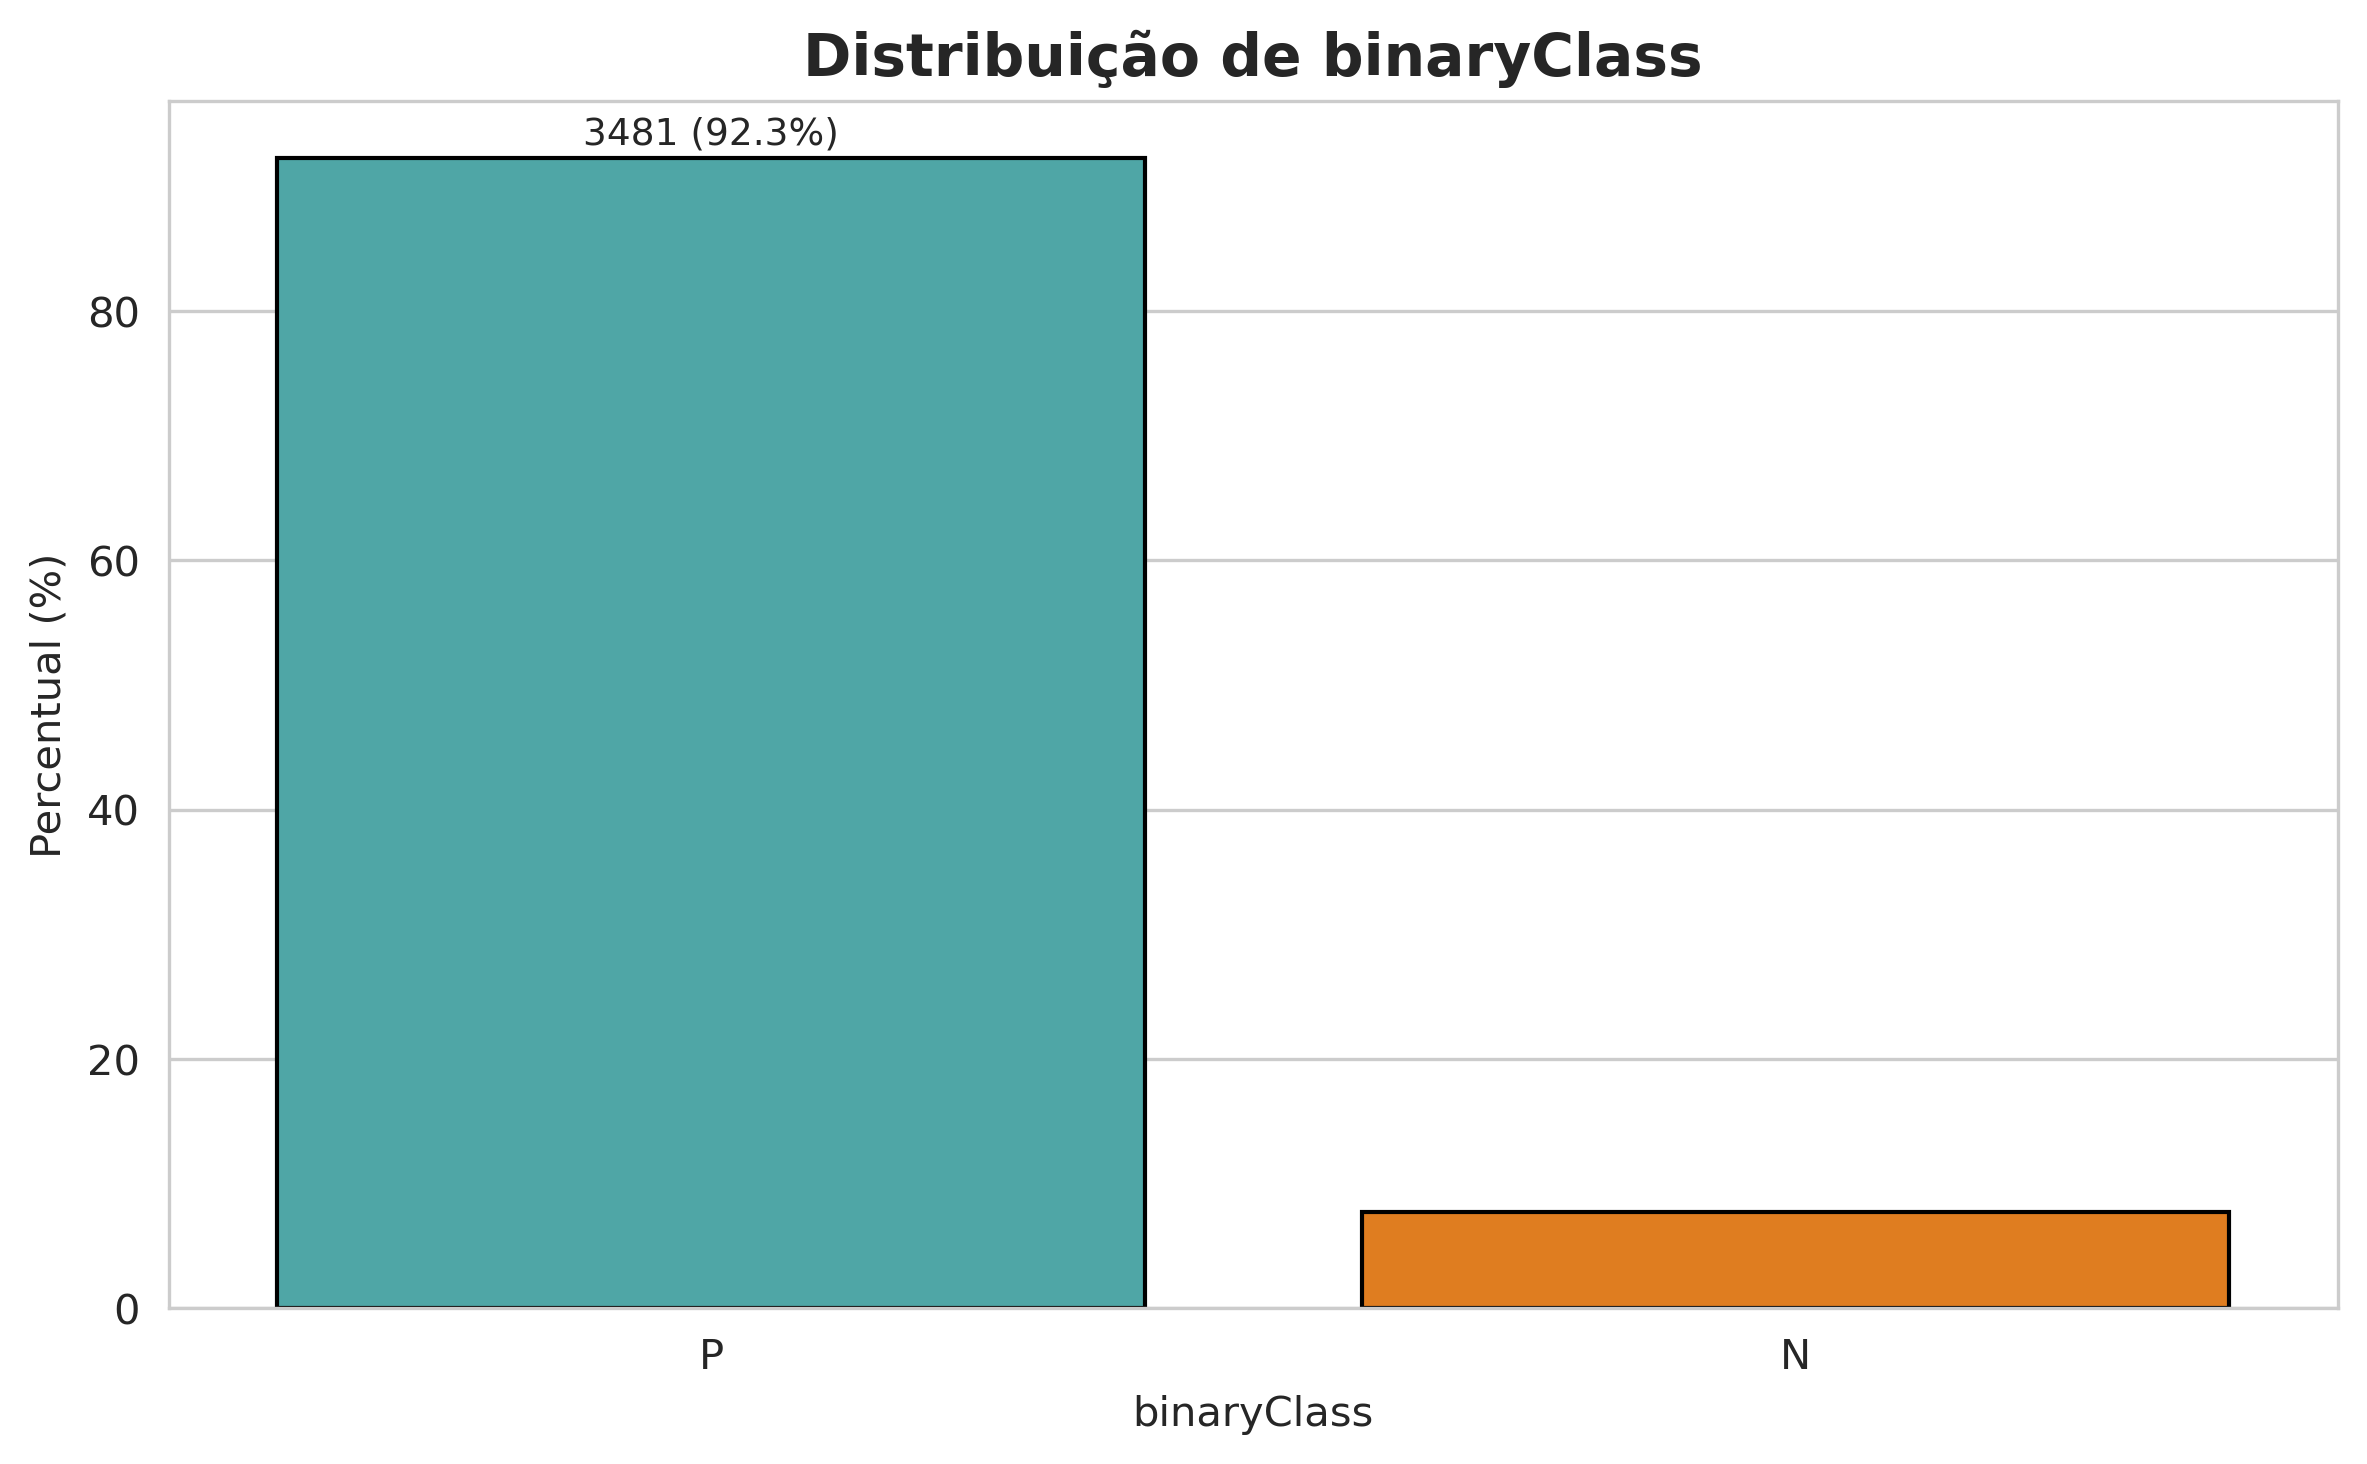
\includegraphics{figuras/eda_03.png}
\caption{Distribuição da variável-alvo}
\end{figure}

O desbalanceamento justifica o uso de métricas que considerem o
comportamento da classe minoritária, especialmente Precision, Recall, F1
e PR-AUC. A acurácia, isoladamente, não seria suficiente para
caracterizar o desempenho dos modelos.

\hypertarget{formulauxe7uxe3o-da-tarefa}{%
\subsubsection{3.2 Formulação da
tarefa}\label{formulauxe7uxe3o-da-tarefa}}

A tarefa foi formulada como classificação binária supervisionada. Os
modelos recebem os atributos disponíveis como preditores e estimam a
classe \texttt{binaryClass}. A classe \texttt{N} foi definida como
positiva para os cálculos de Precision, Recall, F1 e PR-AUC.

Essa formulação reproduz a classificação presente no conjunto de dados.
A interpretação clínica do rótulo depende da documentação de sua
construção, que não foi confirmada de maneira independente neste
trabalho.

\hypertarget{anuxe1lise-exploratuxf3ria-de-dados}{%
\subsection{4. Análise exploratória de
dados}\label{anuxe1lise-exploratuxf3ria-de-dados}}

A análise exploratória foi realizada antes da modelagem para compreender
a estrutura da base, avaliar a qualidade dos dados e identificar padrões
que orientassem a preparação e os experimentos.

\hypertarget{qualidade-inicial-e-registros-duplicados}{%
\subsubsection{4.1 Qualidade inicial e registros
duplicados}\label{qualidade-inicial-e-registros-duplicados}}

A inspeção inicial identificou 61 registros excedentes em grupos de
duplicatas exatas, correspondentes a 33 padrões repetidos. Também foi
identificado um valor de idade igual a 455 anos, considerado inválido e
convertido em ausente na cópia analítica, sem exclusão do registro.

A variável \texttt{TBG} estava integralmente ausente, enquanto
\texttt{TBG\ measured} apresentava apenas uma categoria (\texttt{f}),
sem variabilidade. Essas características fundamentaram a exclusão dessas
duas variáveis da base destinada à modelagem.

\textbf{Figura 2 --- Composição dos registros e duplicidades
identificadas na base original.}

\begin{figure}
\centering
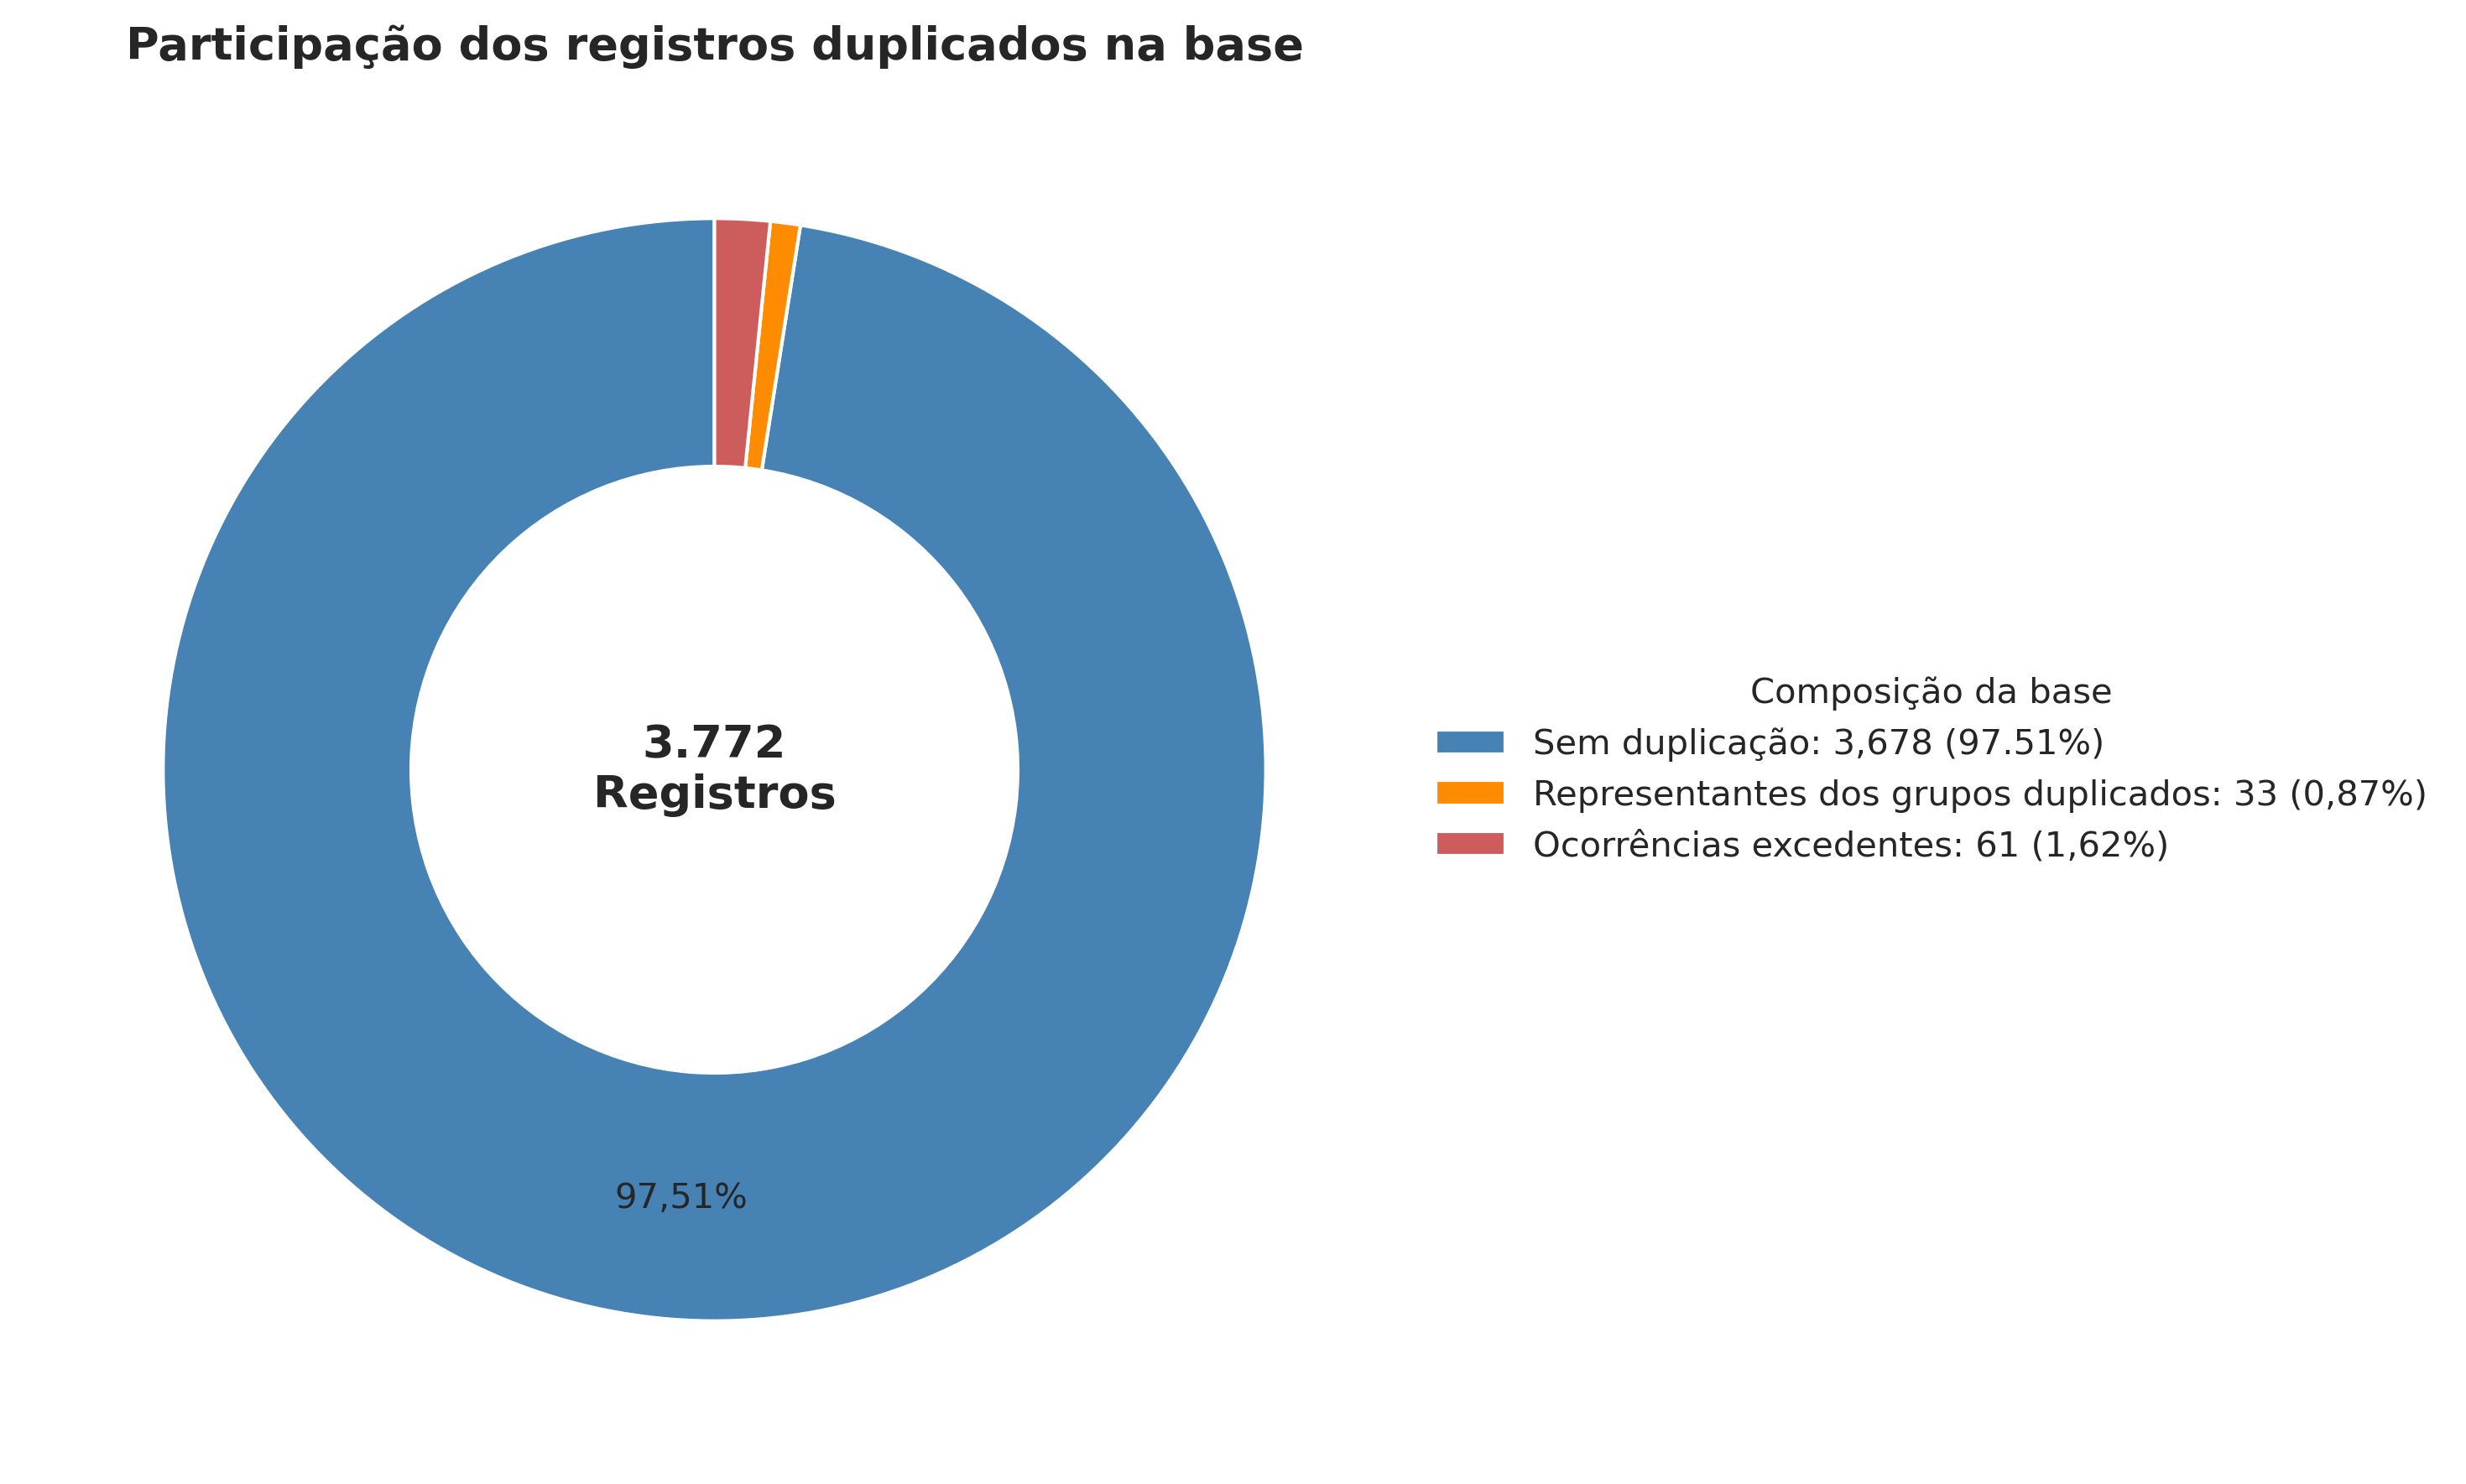
\includegraphics{figuras/eda_02.png}
\caption{Composição e duplicidades}
\end{figure}

\hypertarget{distribuiuxe7uxe3o-das-variuxe1veis-numuxe9ricas}{%
\subsubsection{4.2 Distribuição das variáveis
numéricas}\label{distribuiuxe7uxe3o-das-variuxe1veis-numuxe9ricas}}

As variáveis numéricas foram examinadas por meio de estatísticas
descritivas, histogramas e boxplots. Os exames laboratoriais apresentam
distribuições assimétricas à direita e valores extremos. O TSH se
destaca pela assimetria mais acentuada.

A presença de valores extremos não foi interpretada automaticamente como
erro. Como a análise exploratória não permite determinar se esses
valores são inconsistências ou variações legítimas, eles foram mantidos
inicialmente.

\textbf{Figura 3 --- Distribuição das variáveis numéricas por boxplots.}

\begin{figure}
\centering
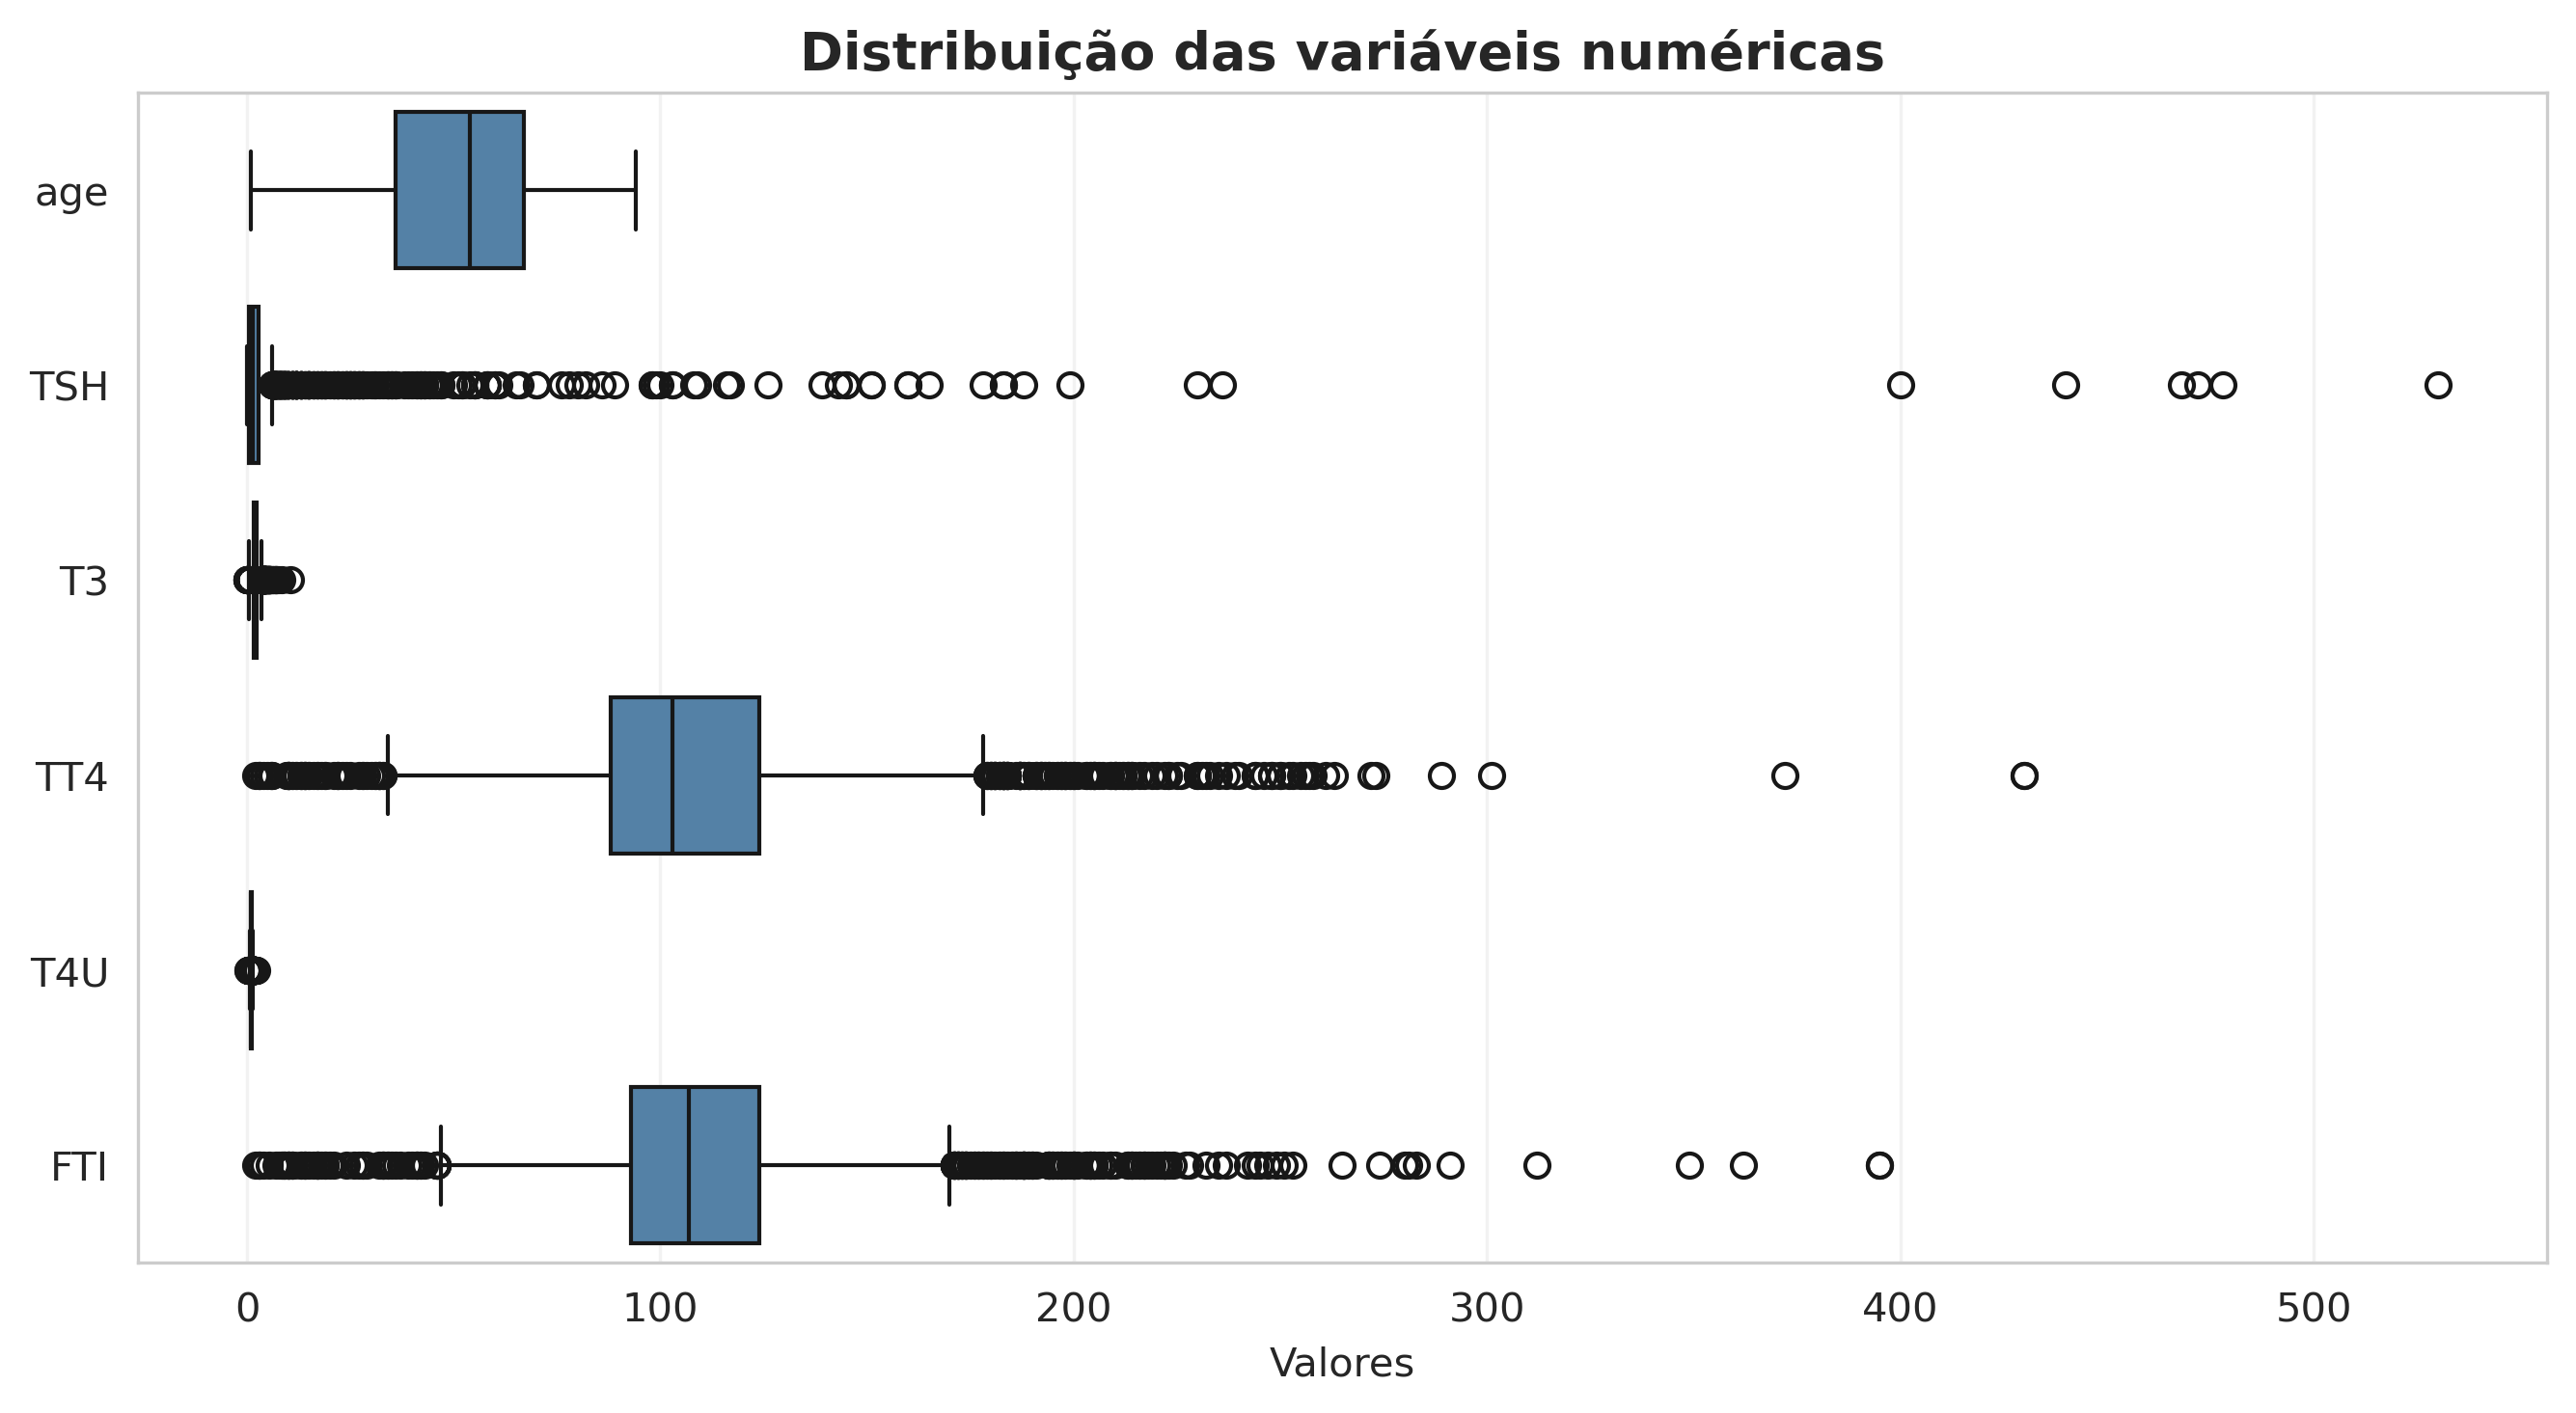
\includegraphics{figuras/eda_04.png}
\caption{Boxplots das variáveis numéricas}
\end{figure}

\textbf{Figura 4 --- Distribuições das variáveis numéricas por
histogramas.}

\begin{figure}
\centering
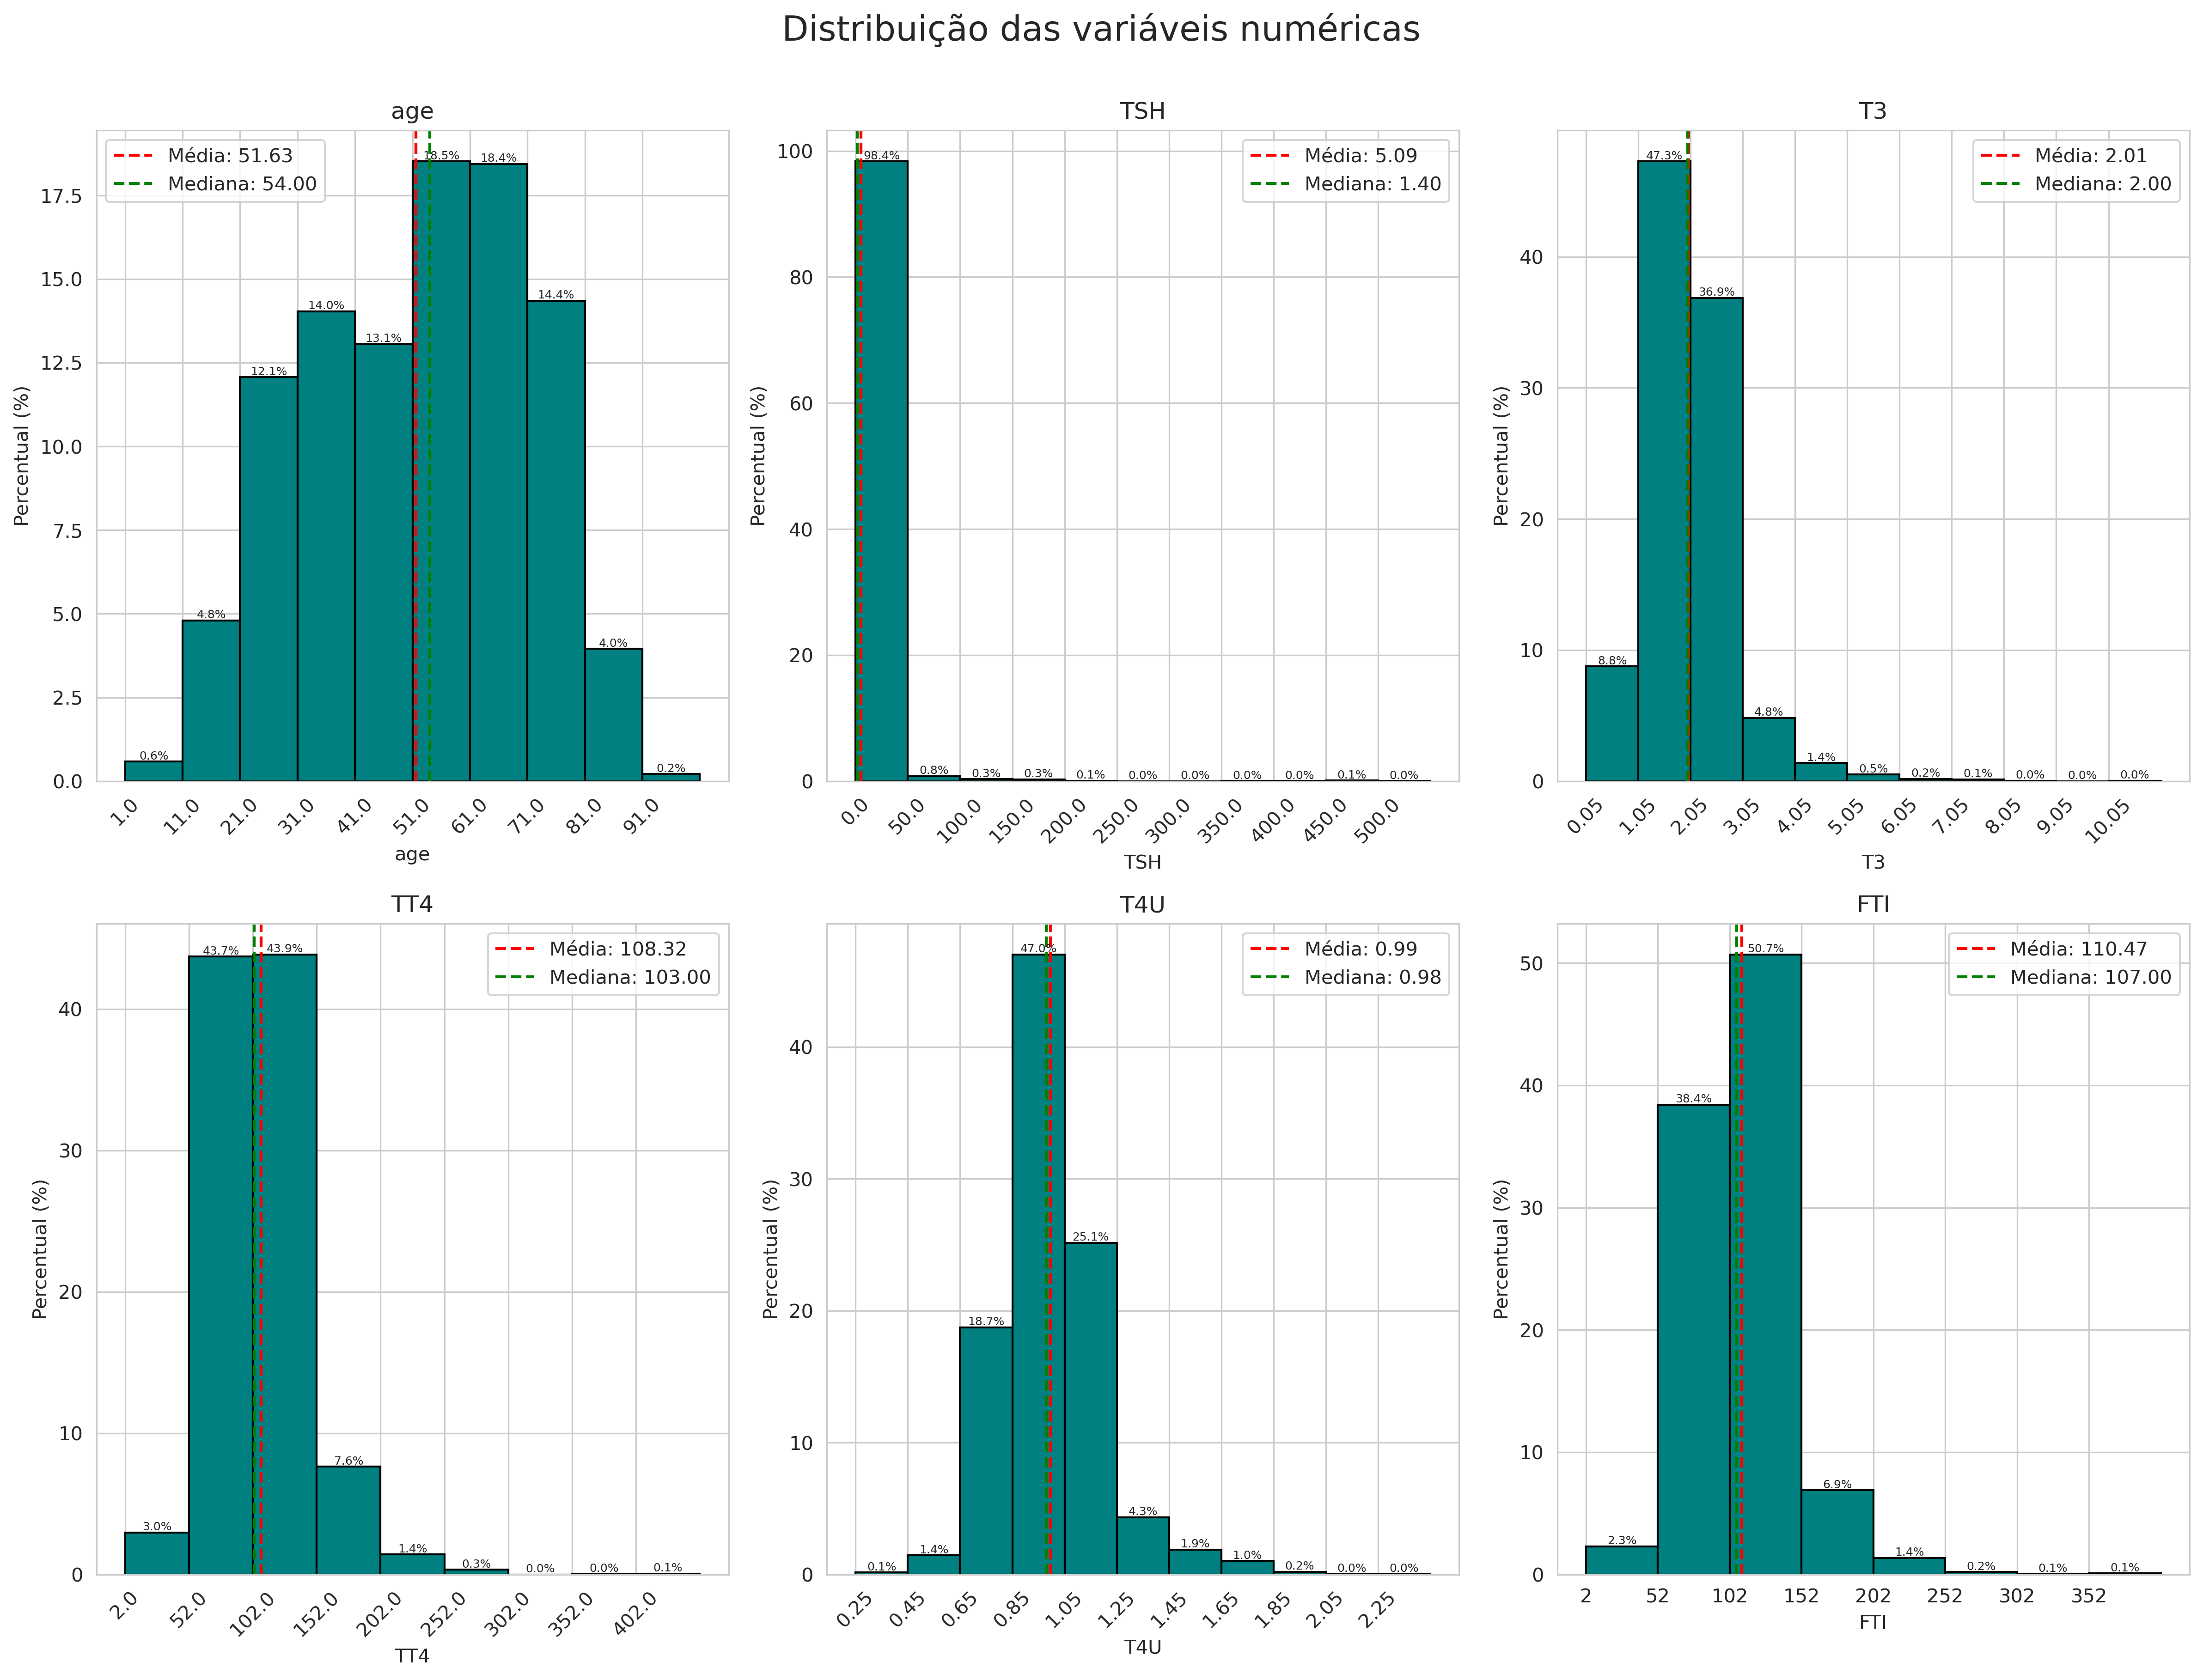
\includegraphics{figuras/eda_05.png}
\caption{Histogramas das variáveis numéricas}
\end{figure}

\textbf{Figura 5 --- Boxplots dos exames laboratoriais.}

\begin{figure}
\centering
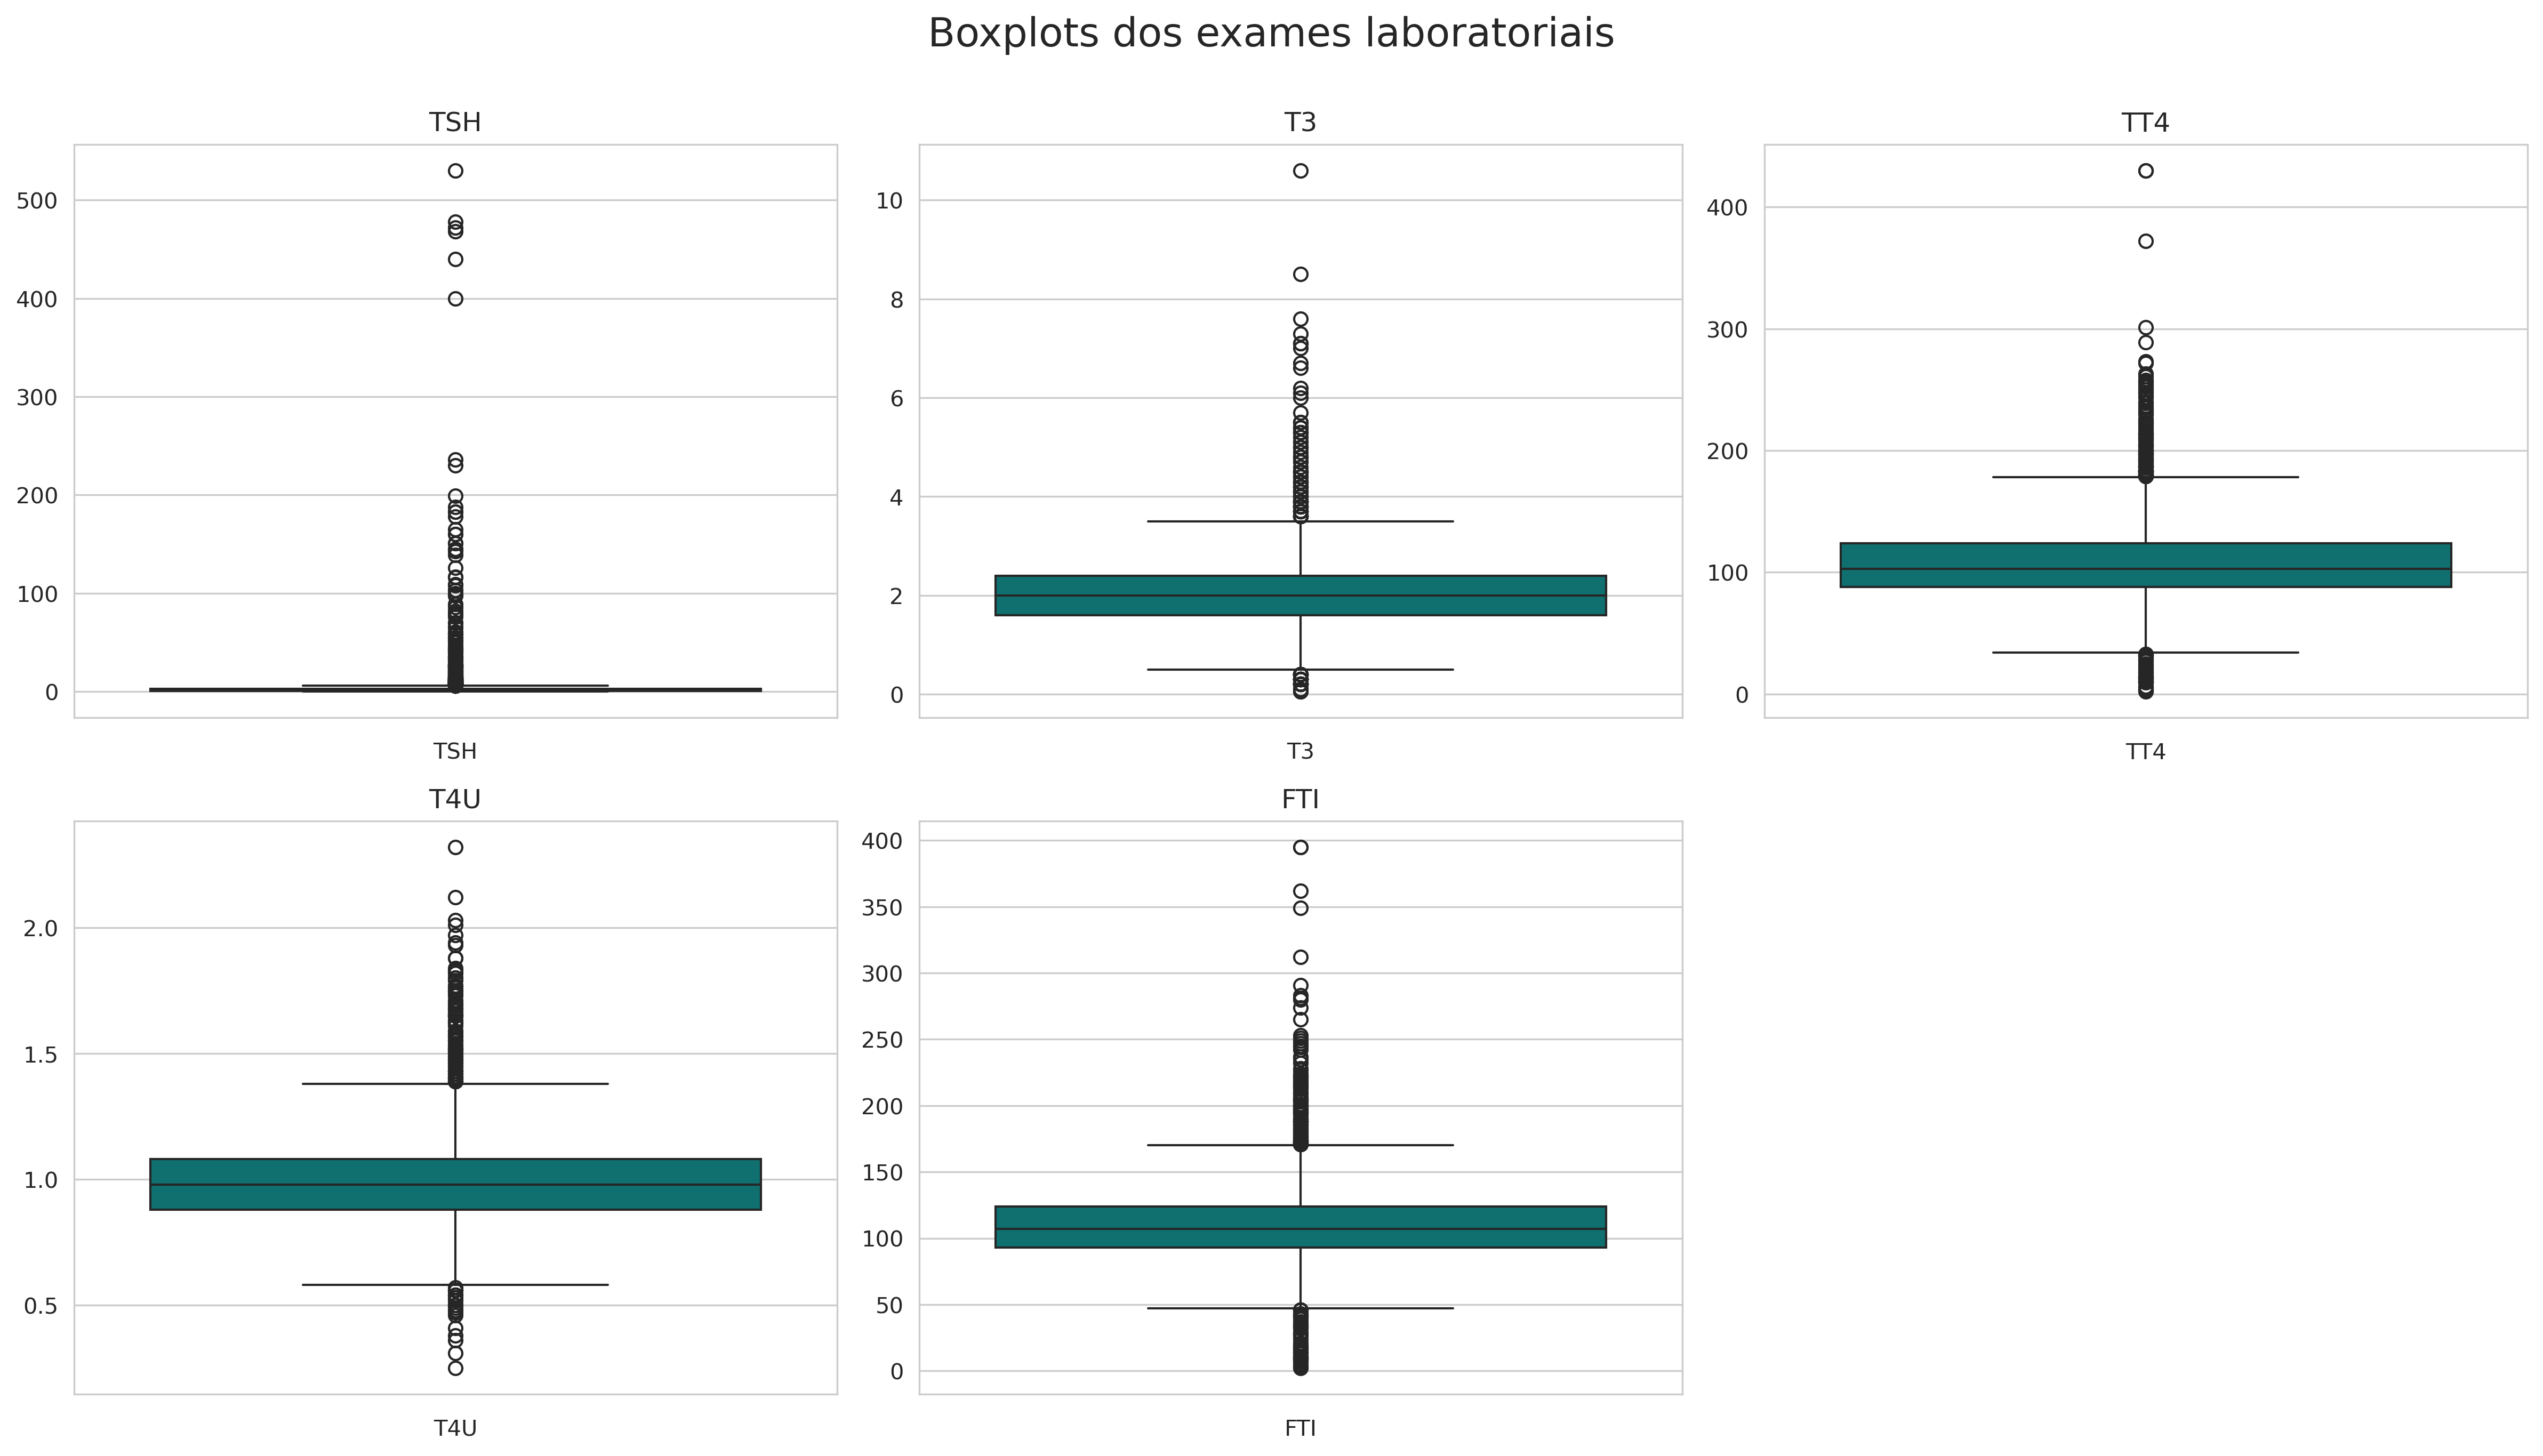
\includegraphics{figuras/eda_06.png}
\caption{Boxplots dos exames laboratoriais}
\end{figure}

\hypertarget{comparauxe7uxe3o-das-variuxe1veis-numuxe9ricas-entre-as-classes}{%
\subsubsection{4.3 Comparação das variáveis numéricas entre as
classes}\label{comparauxe7uxe3o-das-variuxe1veis-numuxe9ricas-entre-as-classes}}

A comparação das estatísticas descritivas mostrou diferenças mais
expressivas nos indicadores laboratoriais do que na idade. A mediana de
TSH foi 12,0 na classe \texttt{N} e 1,2 na classe \texttt{P}. Em sentido
oposto, T3, TT4 e FTI apresentaram medianas menores na classe
\texttt{N}.

A idade apresentou médias próximas entre os grupos: 51,515 anos em
\texttt{N} e 51,638 anos em \texttt{P}. Portanto, nessa exploração, a
idade não apresentou diferença central expressiva entre as classes.

\textbf{Figura 6 --- Distribuição das variáveis numéricas por classe.}

\begin{figure}
\centering
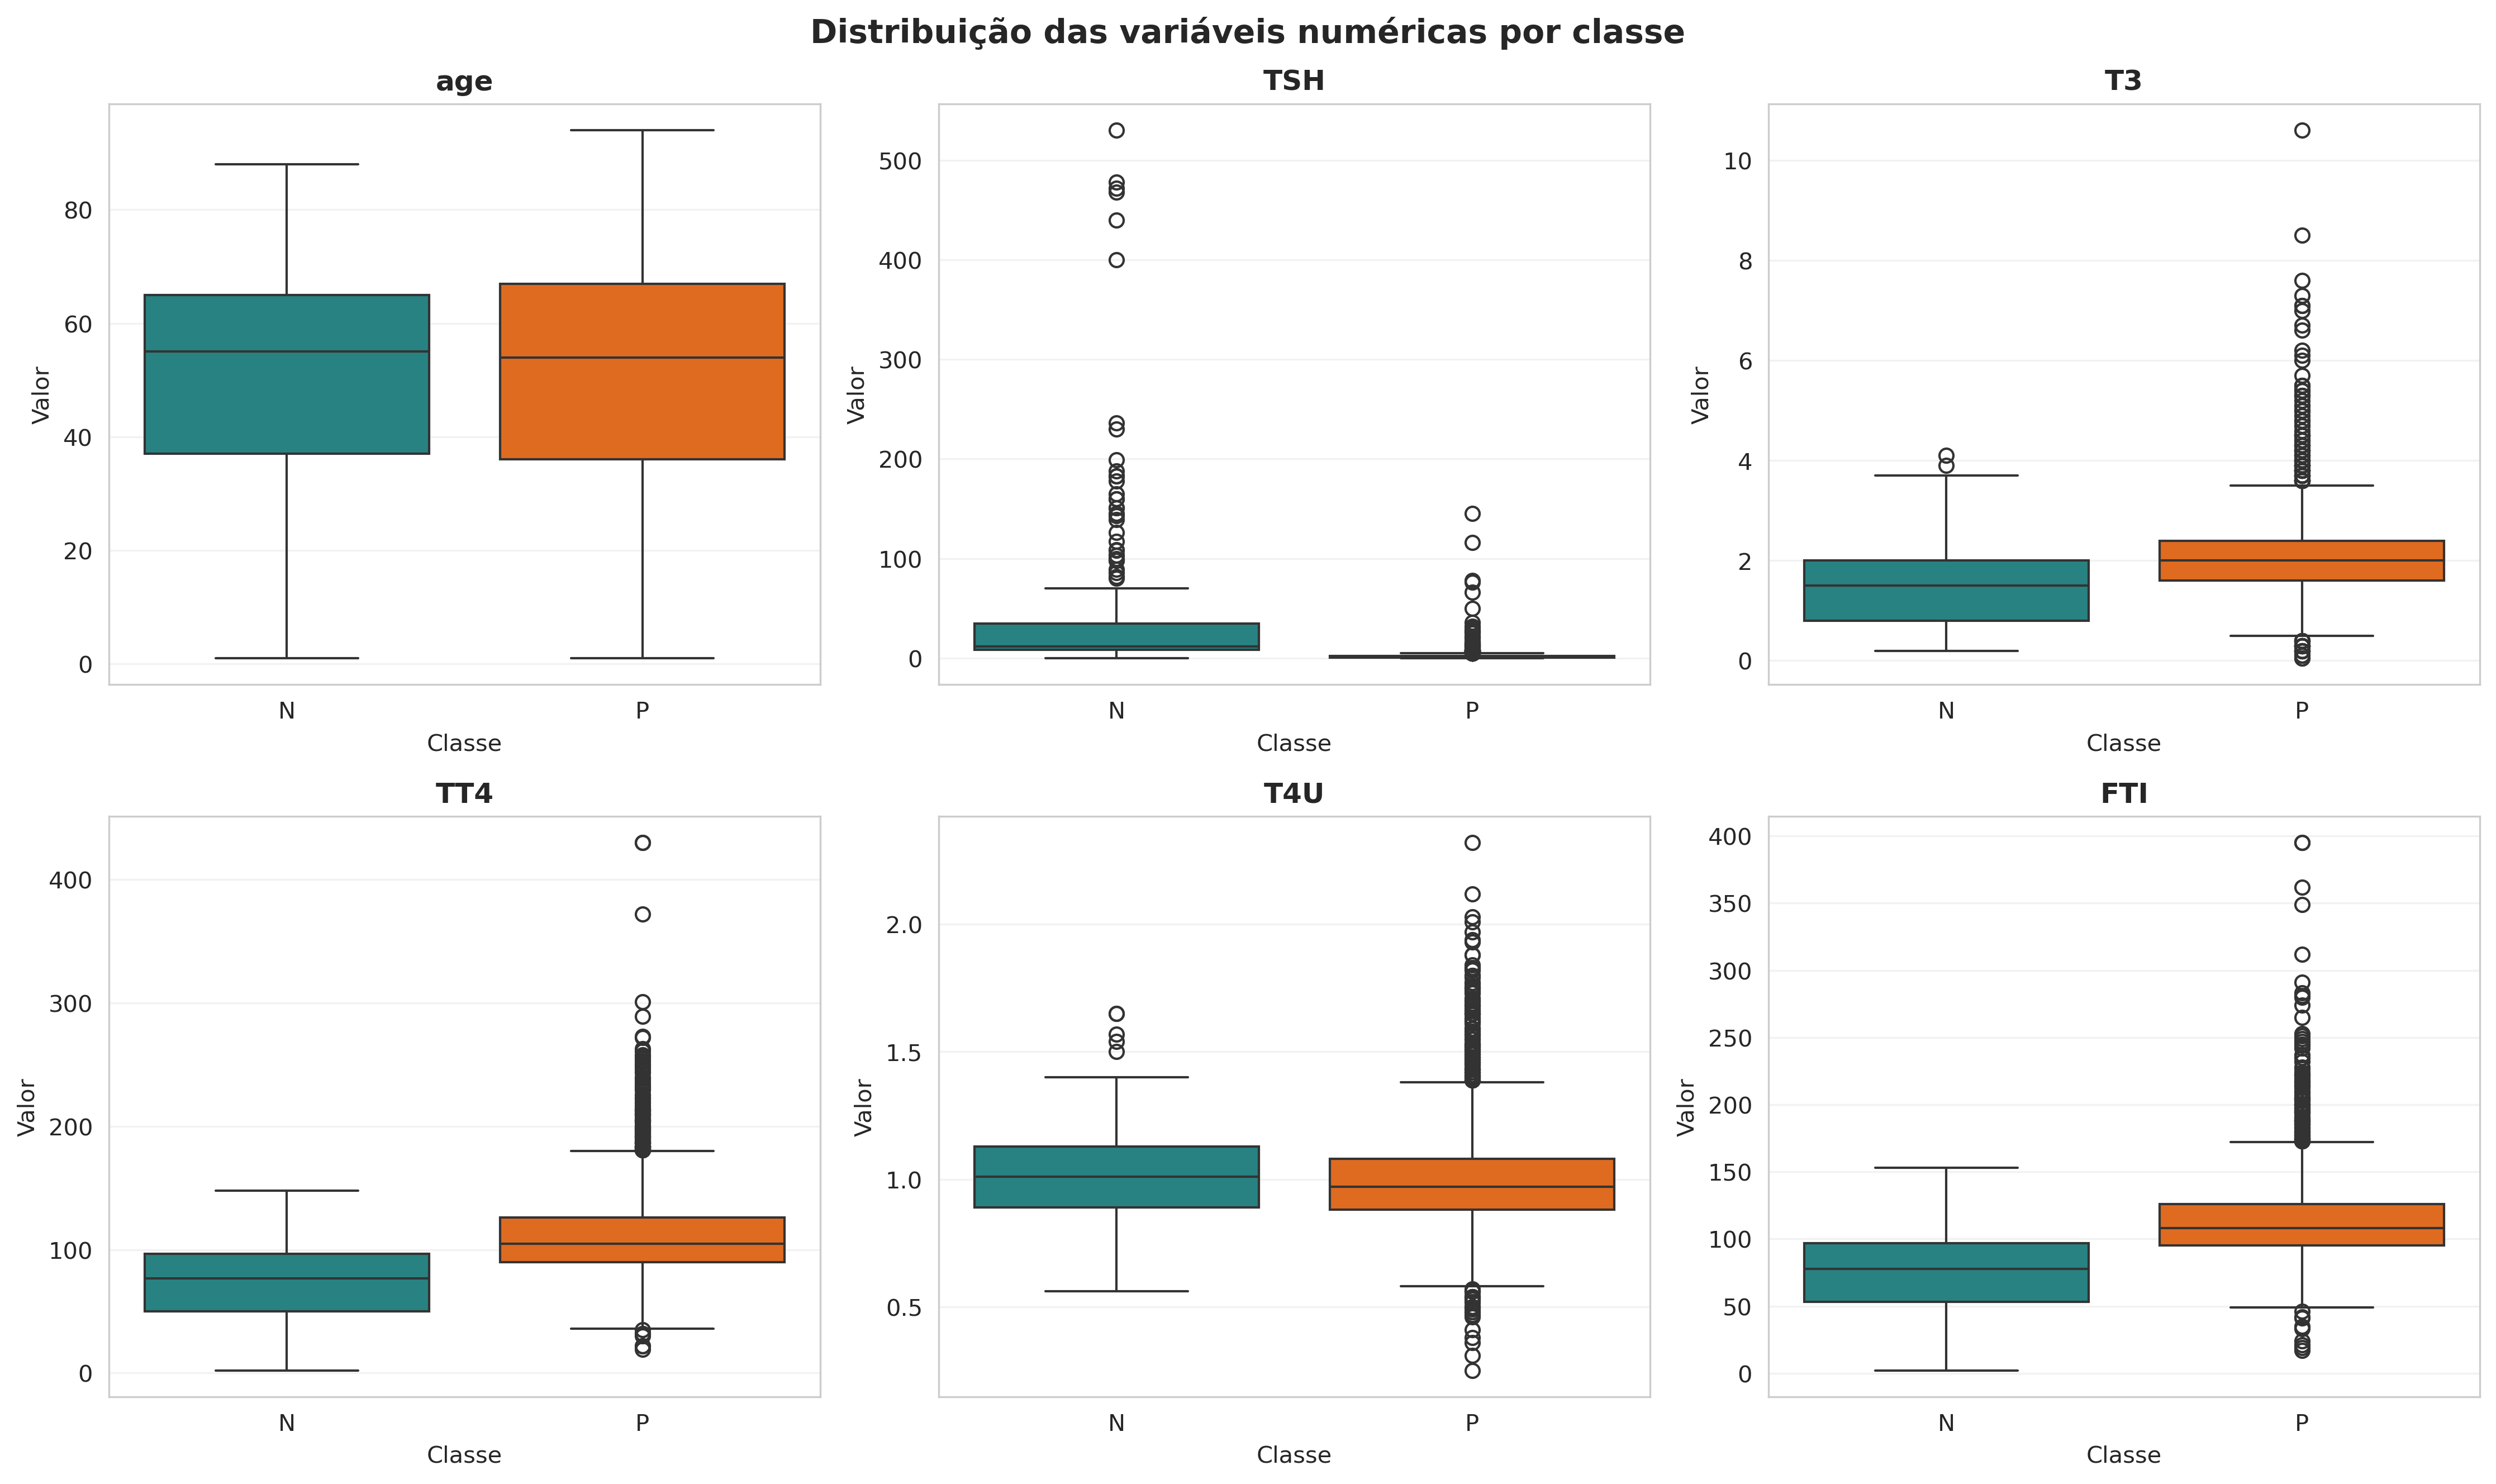
\includegraphics{figuras/eda_07.png}
\caption{Variáveis numéricas por classe}
\end{figure}

\textbf{Figura 7 --- Medianas e intervalos interquartis por classe.}

\begin{figure}
\centering
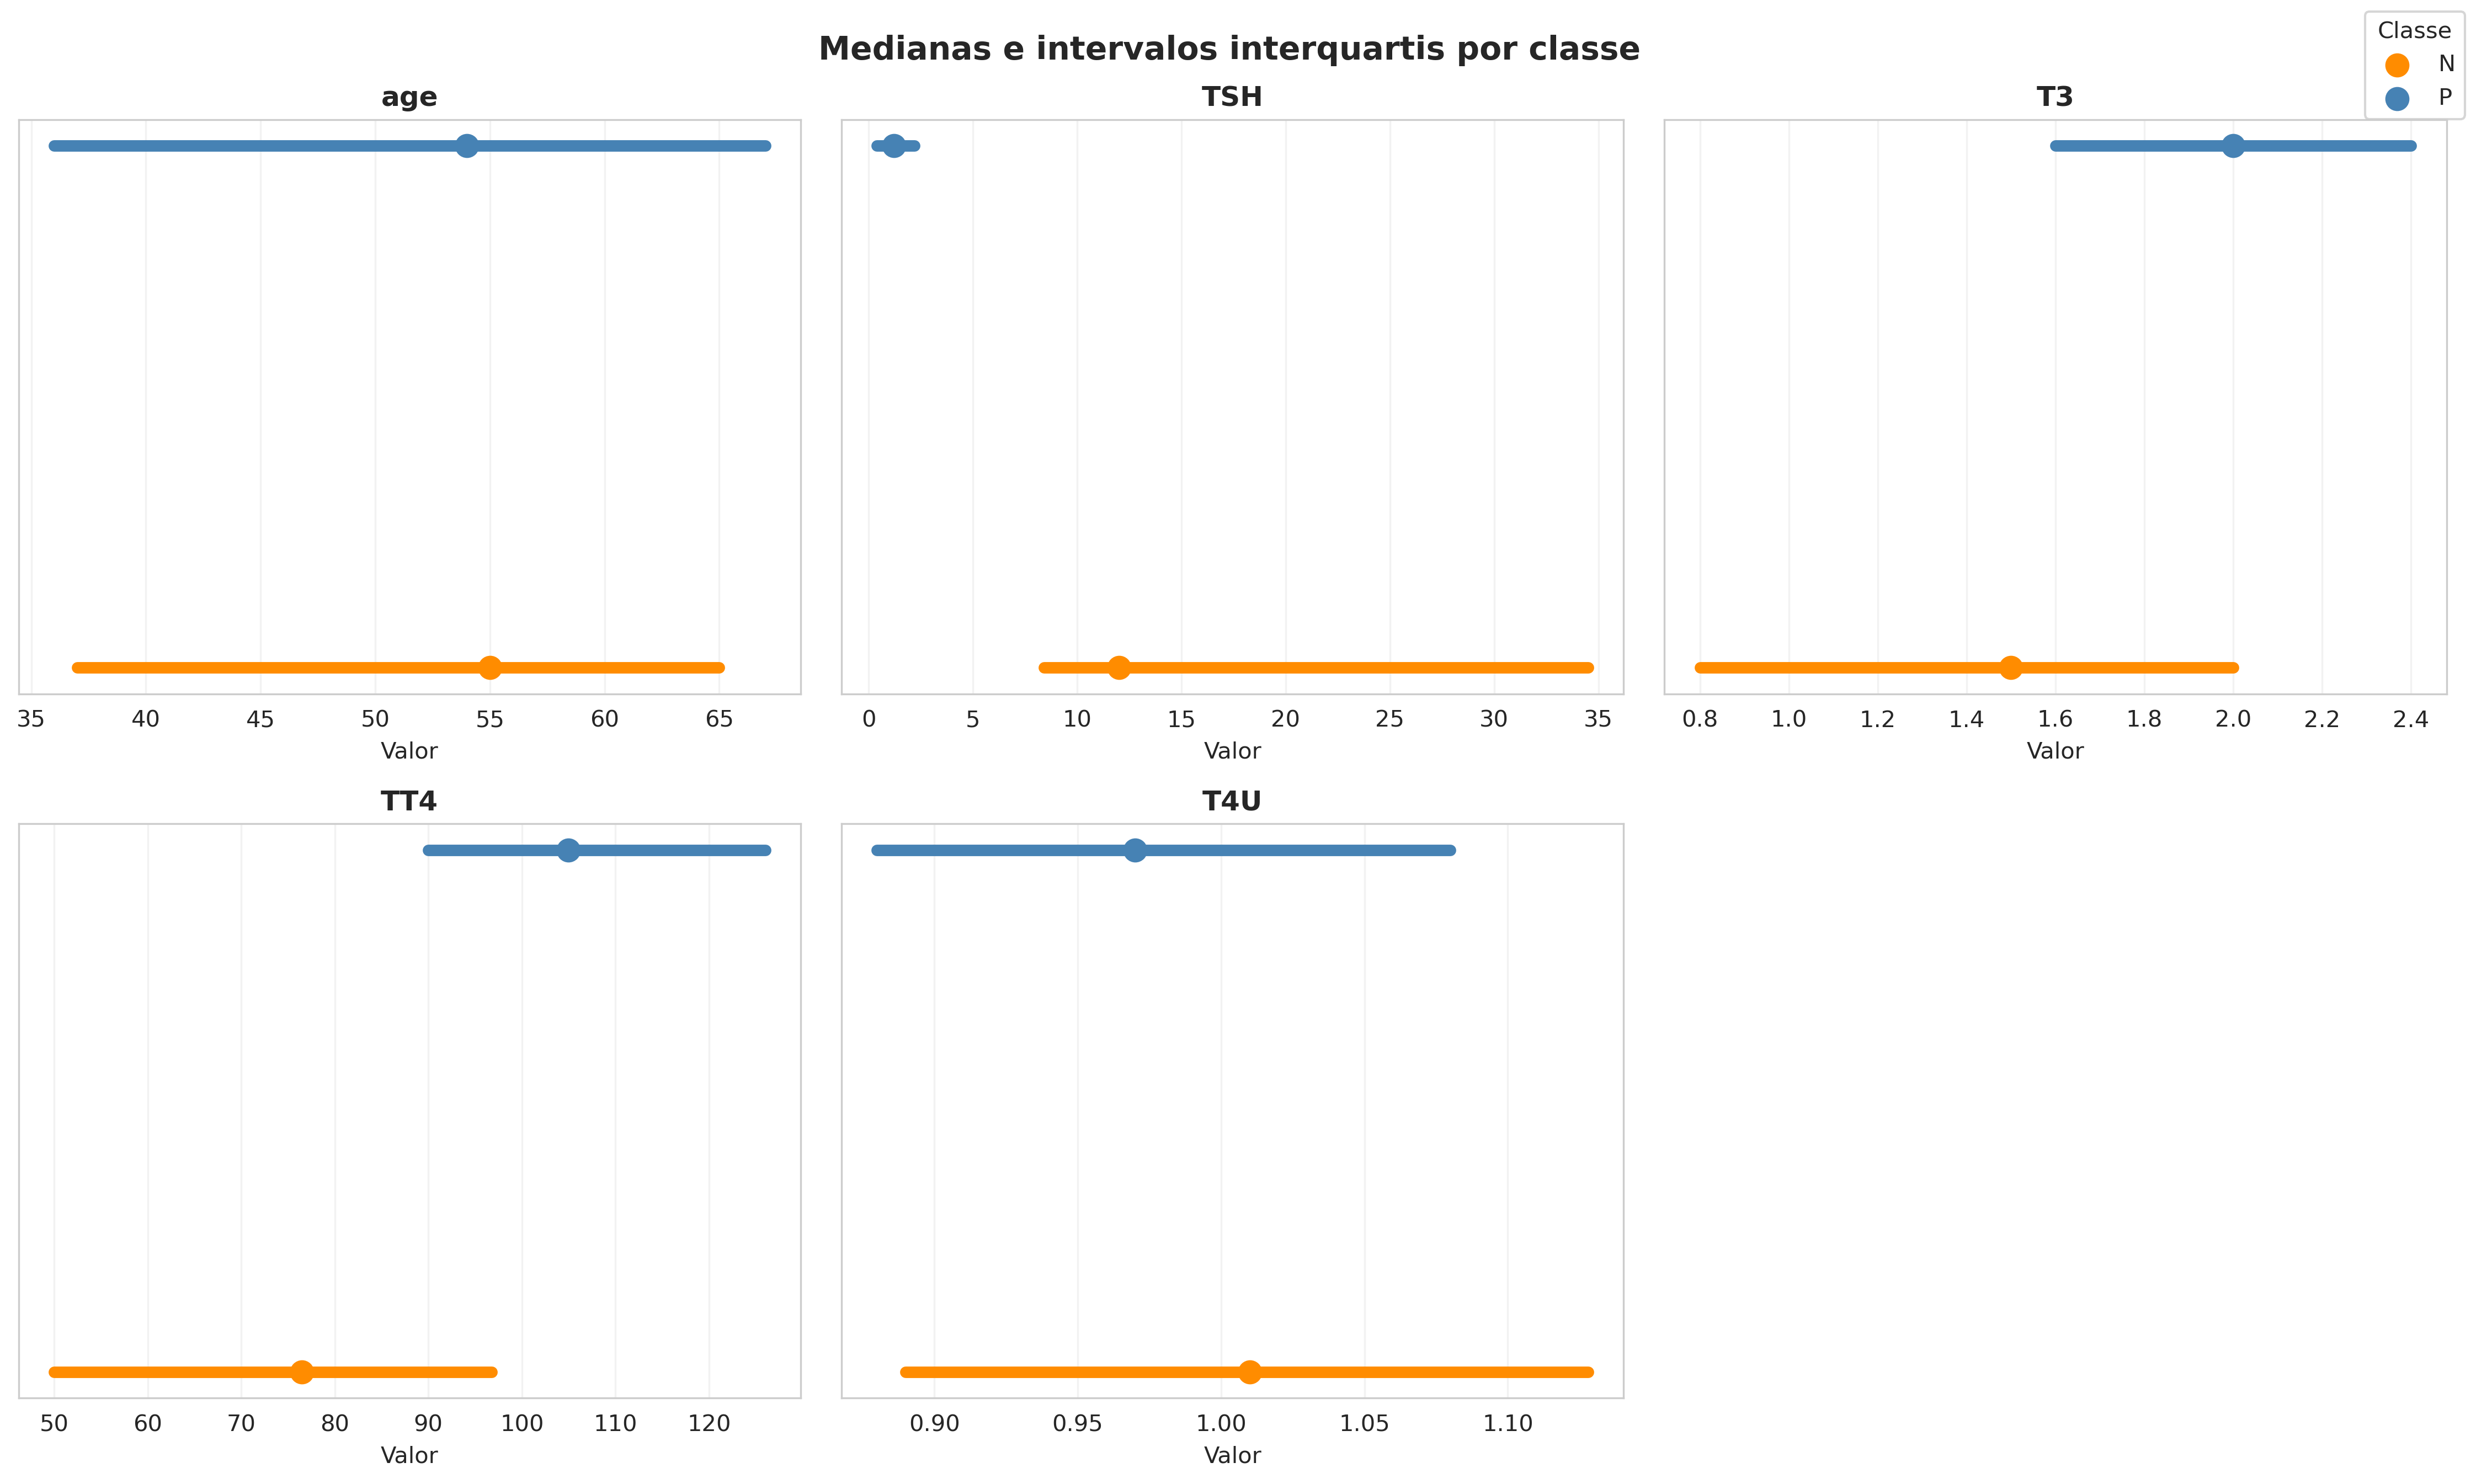
\includegraphics{figuras/eda_08.png}
\caption{Medianas e intervalos interquartis}
\end{figure}

A comparação das medianas reforça a diferença observada em TSH. O
intervalo interquartil dessa variável foi de 8,4 a 34,5 na classe
\texttt{N}, enquanto na classe \texttt{P} variou de 0,4 a 2,2. Para TT4
e FTI, os intervalos interquartis da classe \texttt{N} também se
situaram em níveis inferiores aos da classe \texttt{P}.

Essas diferenças são descritivas e exploratórias. Isoladamente, não
demonstram causalidade nem estabelecem a capacidade preditiva dos
atributos.

\hypertarget{correlauxe7uxe3o-entre-variuxe1veis-numuxe9ricas}{%
\subsubsection{4.4 Correlação entre variáveis
numéricas}\label{correlauxe7uxe3o-entre-variuxe1veis-numuxe9ricas}}

Foi utilizada a correlação de Spearman para investigar associações
monotônicas entre idade e exames laboratoriais, considerando a
assimetria e os valores extremos observados.

A maior correlação positiva ocorreu entre TT4 e FTI (0,742). Também
foram observadas correlações entre T3 e T4U (0,447), TT4 e T4U (0,430) e
T3 e TT4 (0,418). A relação entre TSH e FTI foi negativa e moderada
(-0,412), enquanto idade e T3 apresentaram correlação de -0,290.

\textbf{Figura 8 --- Matriz de correlação de Spearman entre as variáveis
numéricas.}

\begin{figure}
\centering
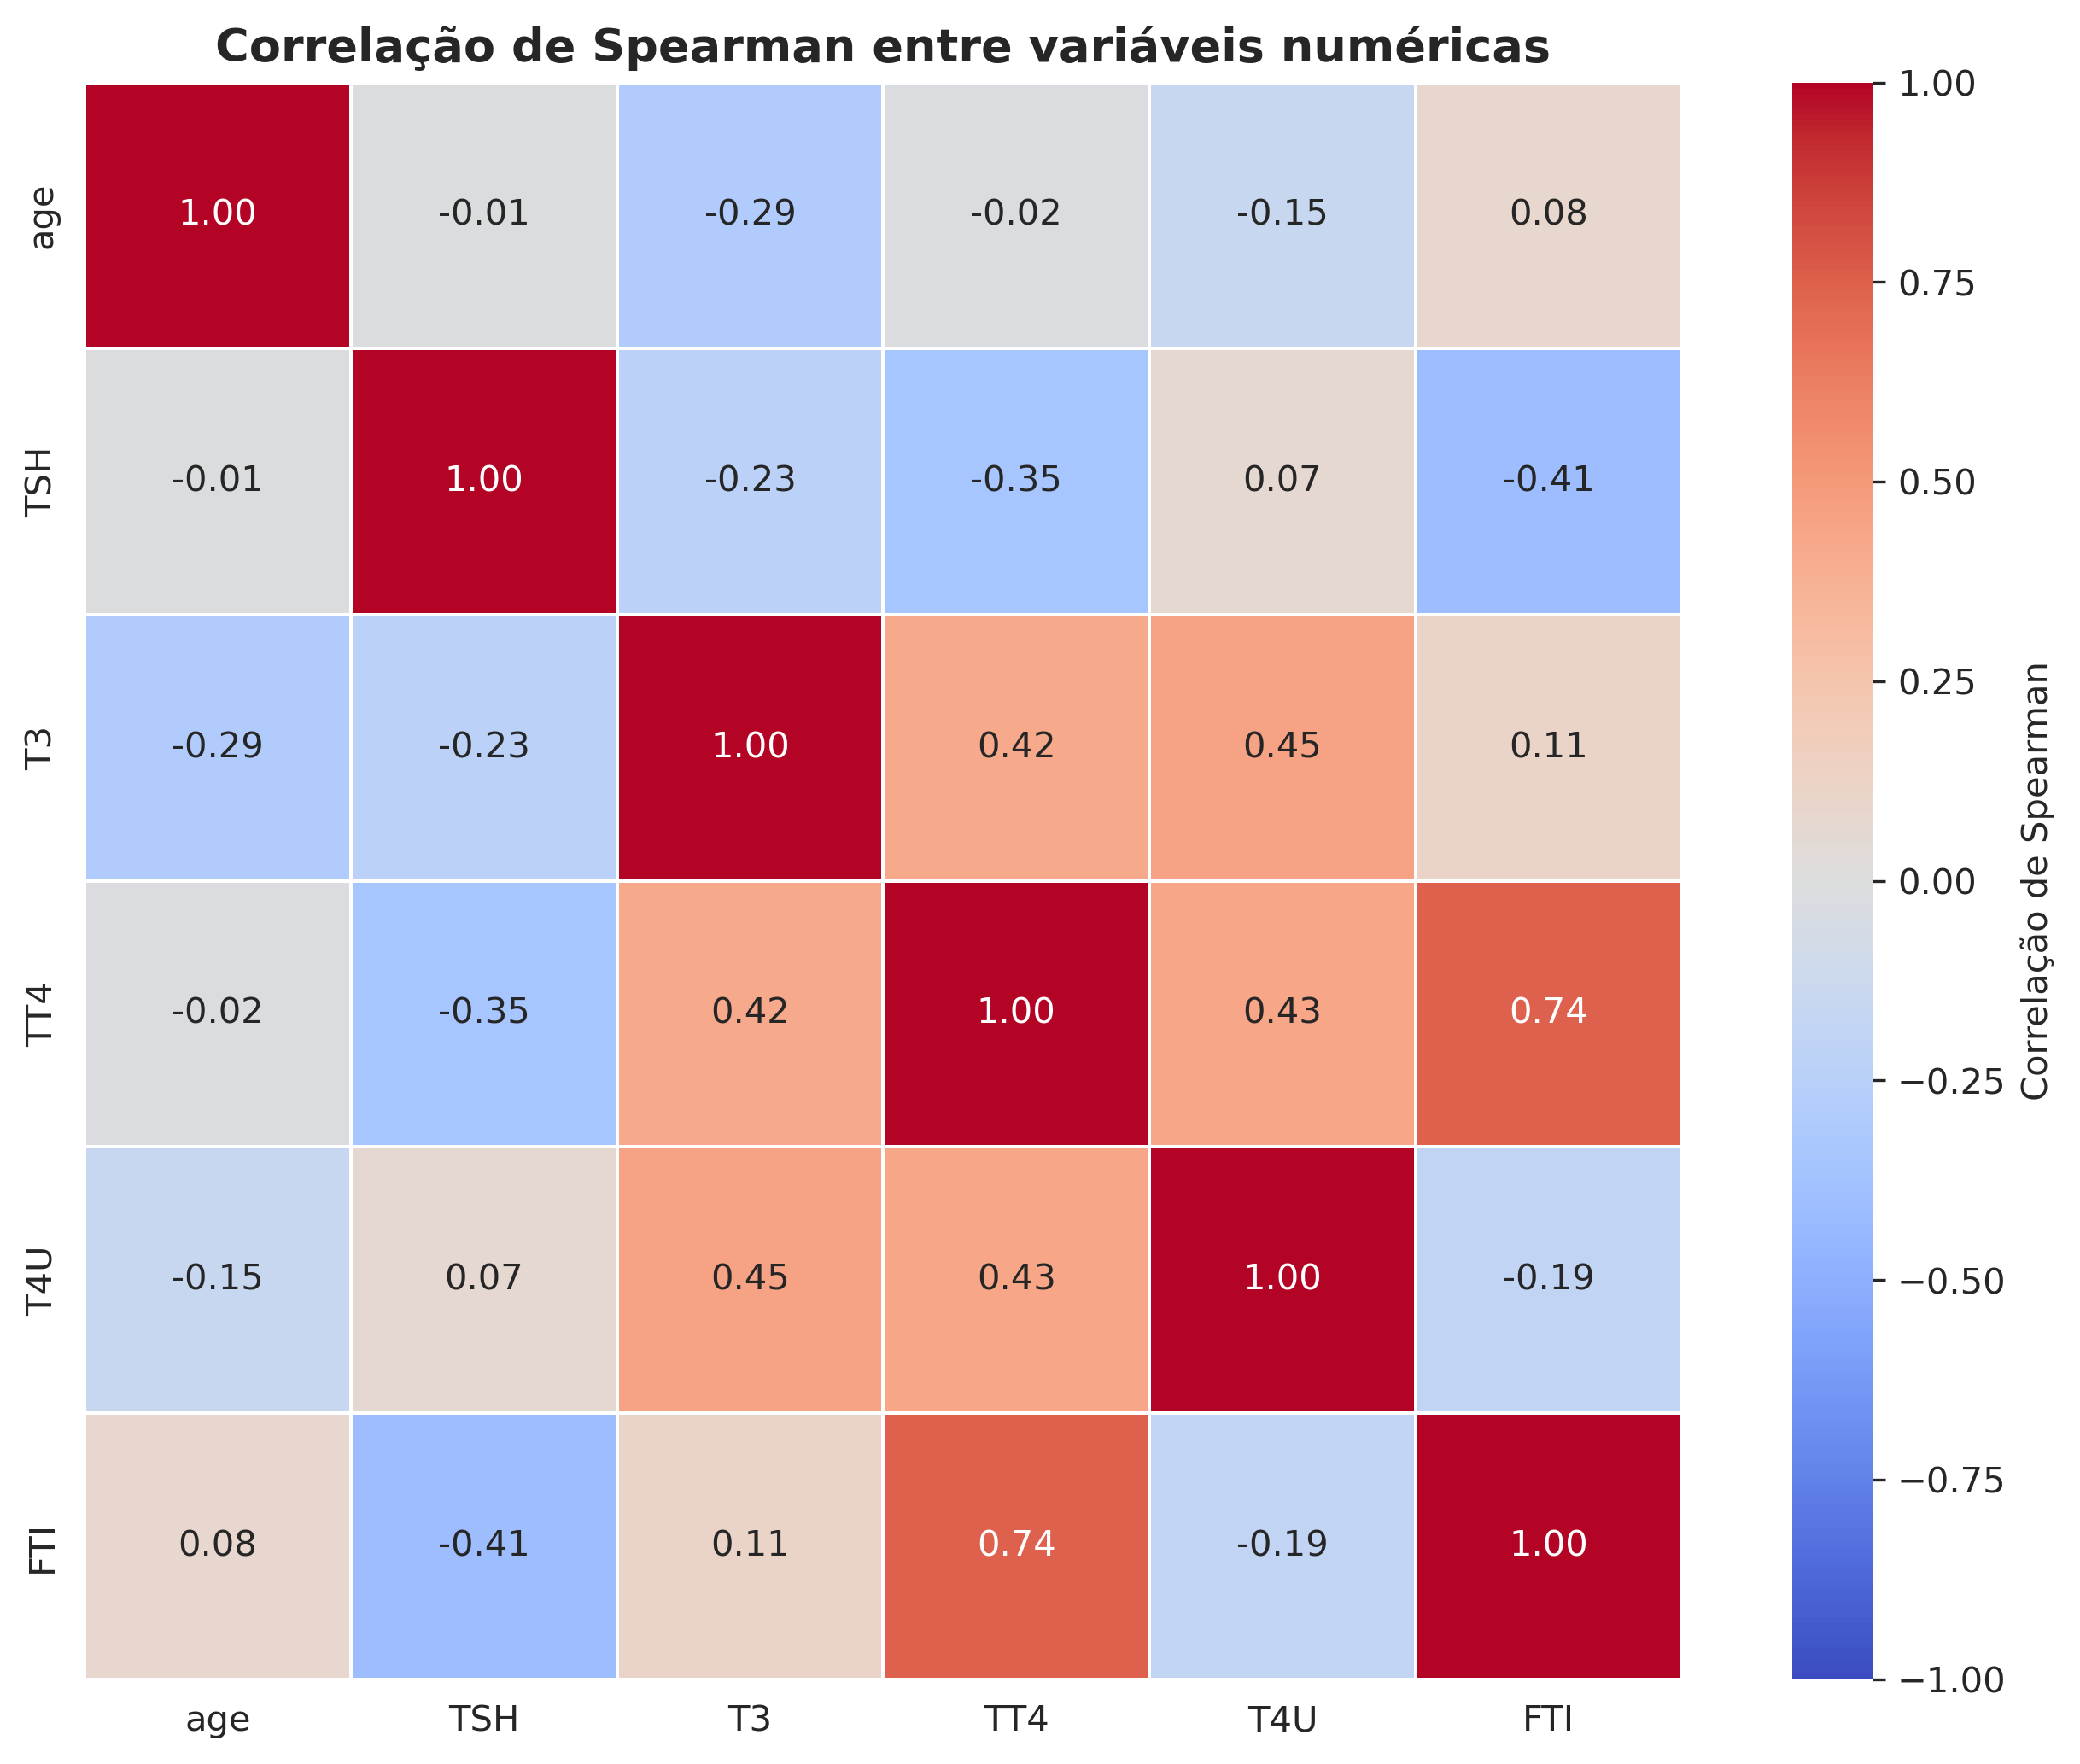
\includegraphics{figuras/eda_09.png}
\caption{Matriz de correlação de Spearman}
\end{figure}

A associação entre TT4 e FTI indica sobreposição de informação entre
esses indicadores. Essa característica deve ser considerada na
interpretação da importância dos preditores. Correlação, entretanto, não
implica causalidade.

\hypertarget{valores-ausentes-e-assimetria}{%
\subsubsection{4.5 Valores ausentes e
assimetria}\label{valores-ausentes-e-assimetria}}

Entre as variáveis numéricas, T3 apresentou a maior proporção de valores
ausentes (20,39\%), seguida por T4U (10,26\%), FTI (10,21\%) e TSH
(9,78\%). A idade apresentou duas observações ausentes após o tratamento
do valor inválido.

O TSH também apresentou a maior assimetria positiva, com coeficiente de
13,883. As demais variáveis laboratoriais apresentaram assimetria
positiva entre 1,233 e 1,731, enquanto a idade apresentou assimetria
ligeiramente negativa (-0,211).

\textbf{Figura 9 --- Assimetria e percentual de valores ausentes nas
variáveis numéricas.}

\begin{figure}
\centering
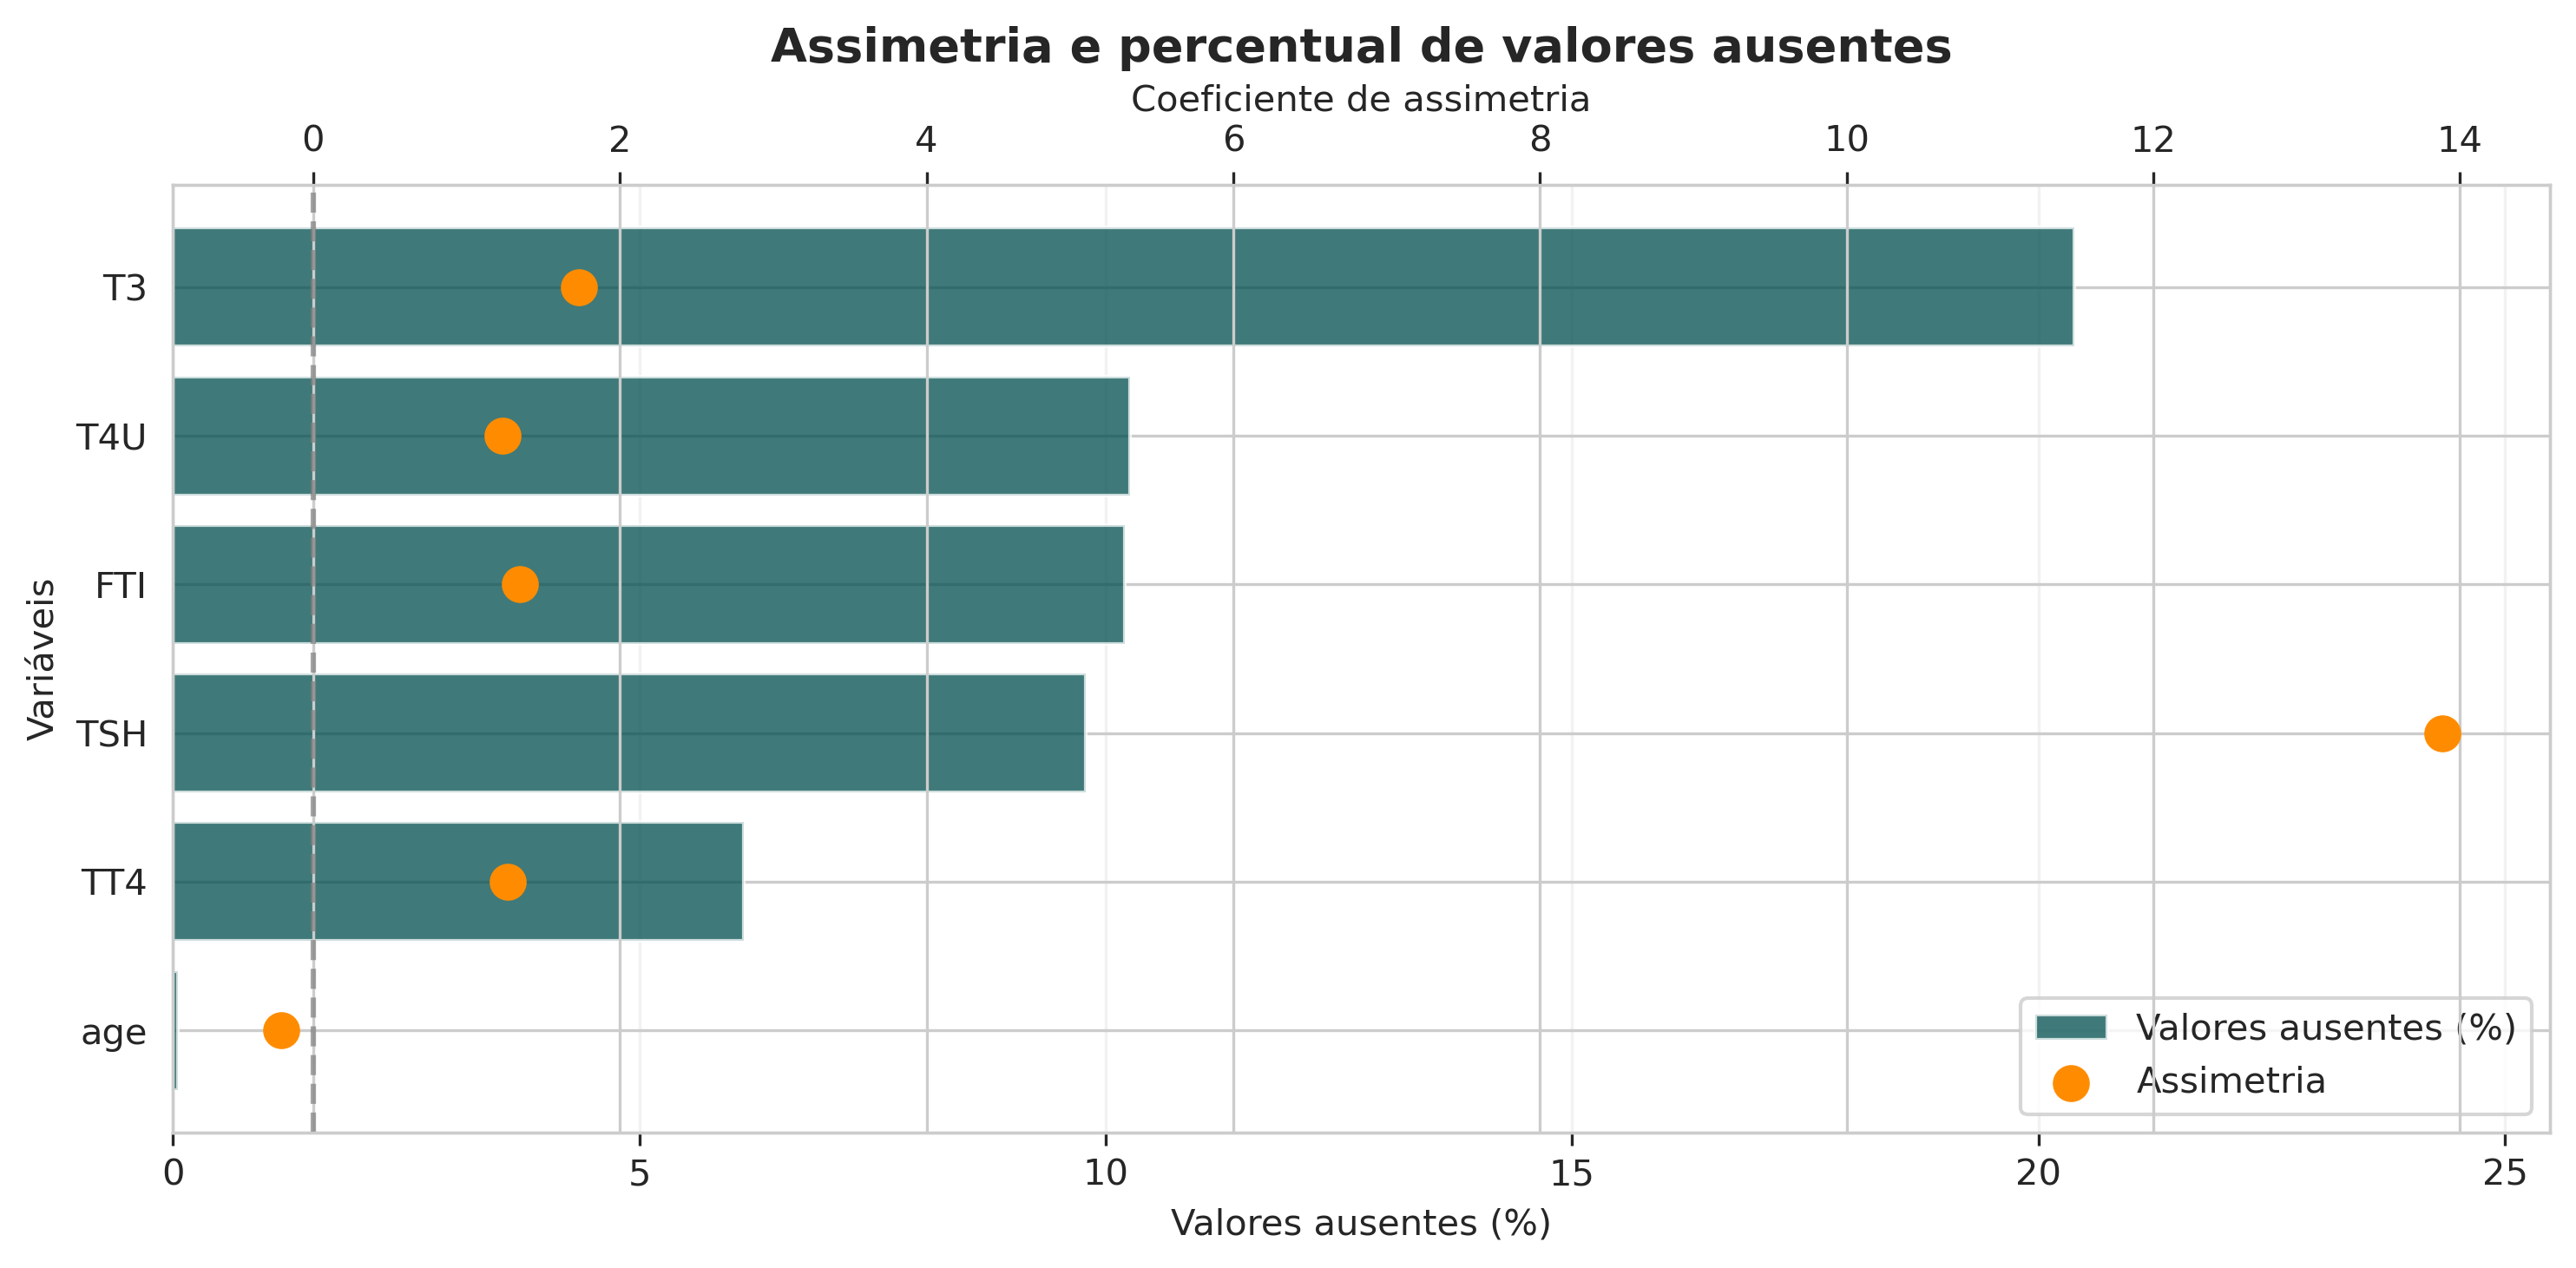
\includegraphics{figuras/eda_10.png}
\caption{Assimetria e valores ausentes}
\end{figure}

A análise conjunta indica que a imputação seria necessária para utilizar
os atributos com ausências nos pipelines de modelagem. Também reforça a
necessidade de cautela na interpretação das distribuições laboratoriais.

\hypertarget{variuxe1veis-categuxf3ricas}{%
\subsubsection{4.6 Variáveis
categóricas}\label{variuxe1veis-categuxf3ricas}}

A classe \texttt{P} predominou em praticamente todas as categorias.
Ainda assim, algumas diferenças na composição foram observadas. Entre os
registros com \texttt{query\ hypothyroid\ =\ t}, por exemplo, a classe
\texttt{N} representou 16,67\%, proporção superior à distribuição geral.
Entre os registros sem medição de TSH (\texttt{TSH\ measured\ =\ f}),
todos pertenciam à classe \texttt{P}.

Algumas categorias apresentaram baixa frequência, como
\texttt{hypopituitary\ =\ t} (1 registro), \texttt{lithium\ =\ t} (18
registros) e \texttt{goitre\ =\ t} (34 registros). Essas frequências
reduzidas exigem cautela na interpretação das proporções.

\textbf{Figura 10 --- Composição percentual das classes nas variáveis
clínicas e categóricas.}

\begin{figure}
\centering
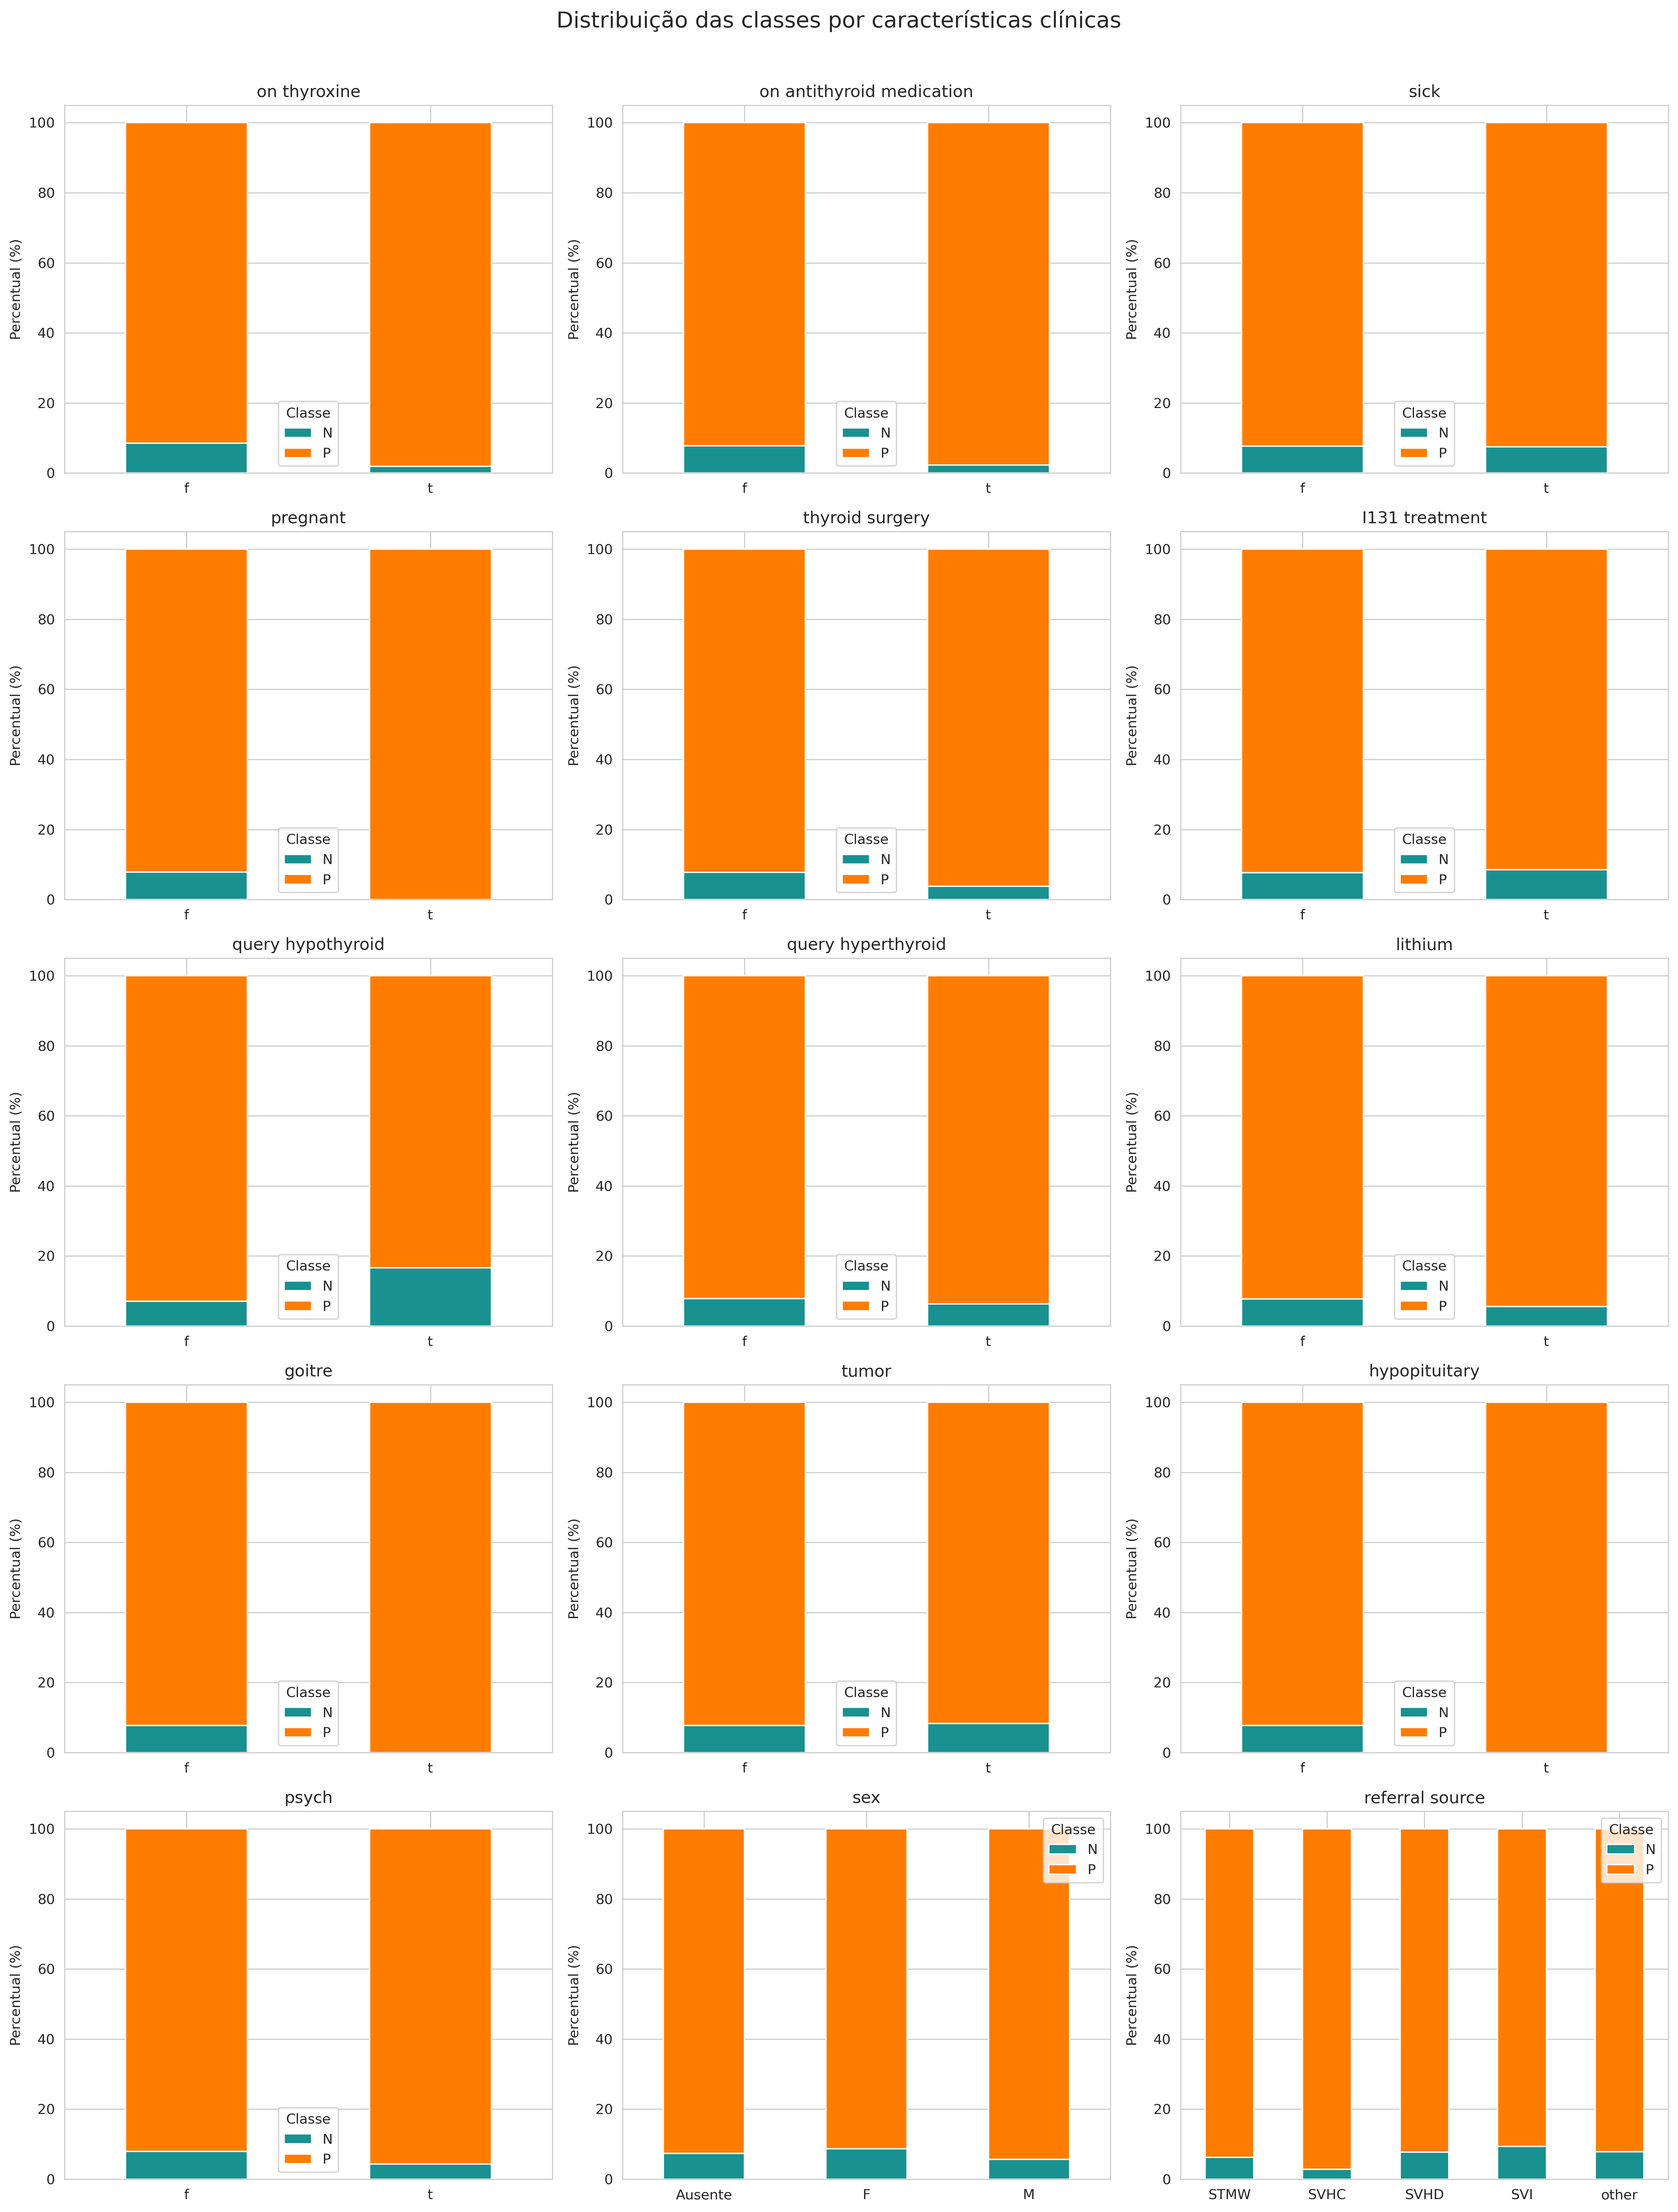
\includegraphics{figuras/eda_11.png}
\caption{Composição das classes por categorias}
\end{figure}

A variável \texttt{sex} apresentou 150 valores ausentes (3,98\%). A
maioria das variáveis categóricas possuía duas categorias, enquanto
\texttt{referral\ source} apresentava cinco. A variável
\texttt{TBG\ measured} era constante, reforçando sua exclusão da
modelagem.

\textbf{Figura 11 --- Concentração da categoria mais frequente por
variável categórica.}

\begin{figure}
\centering
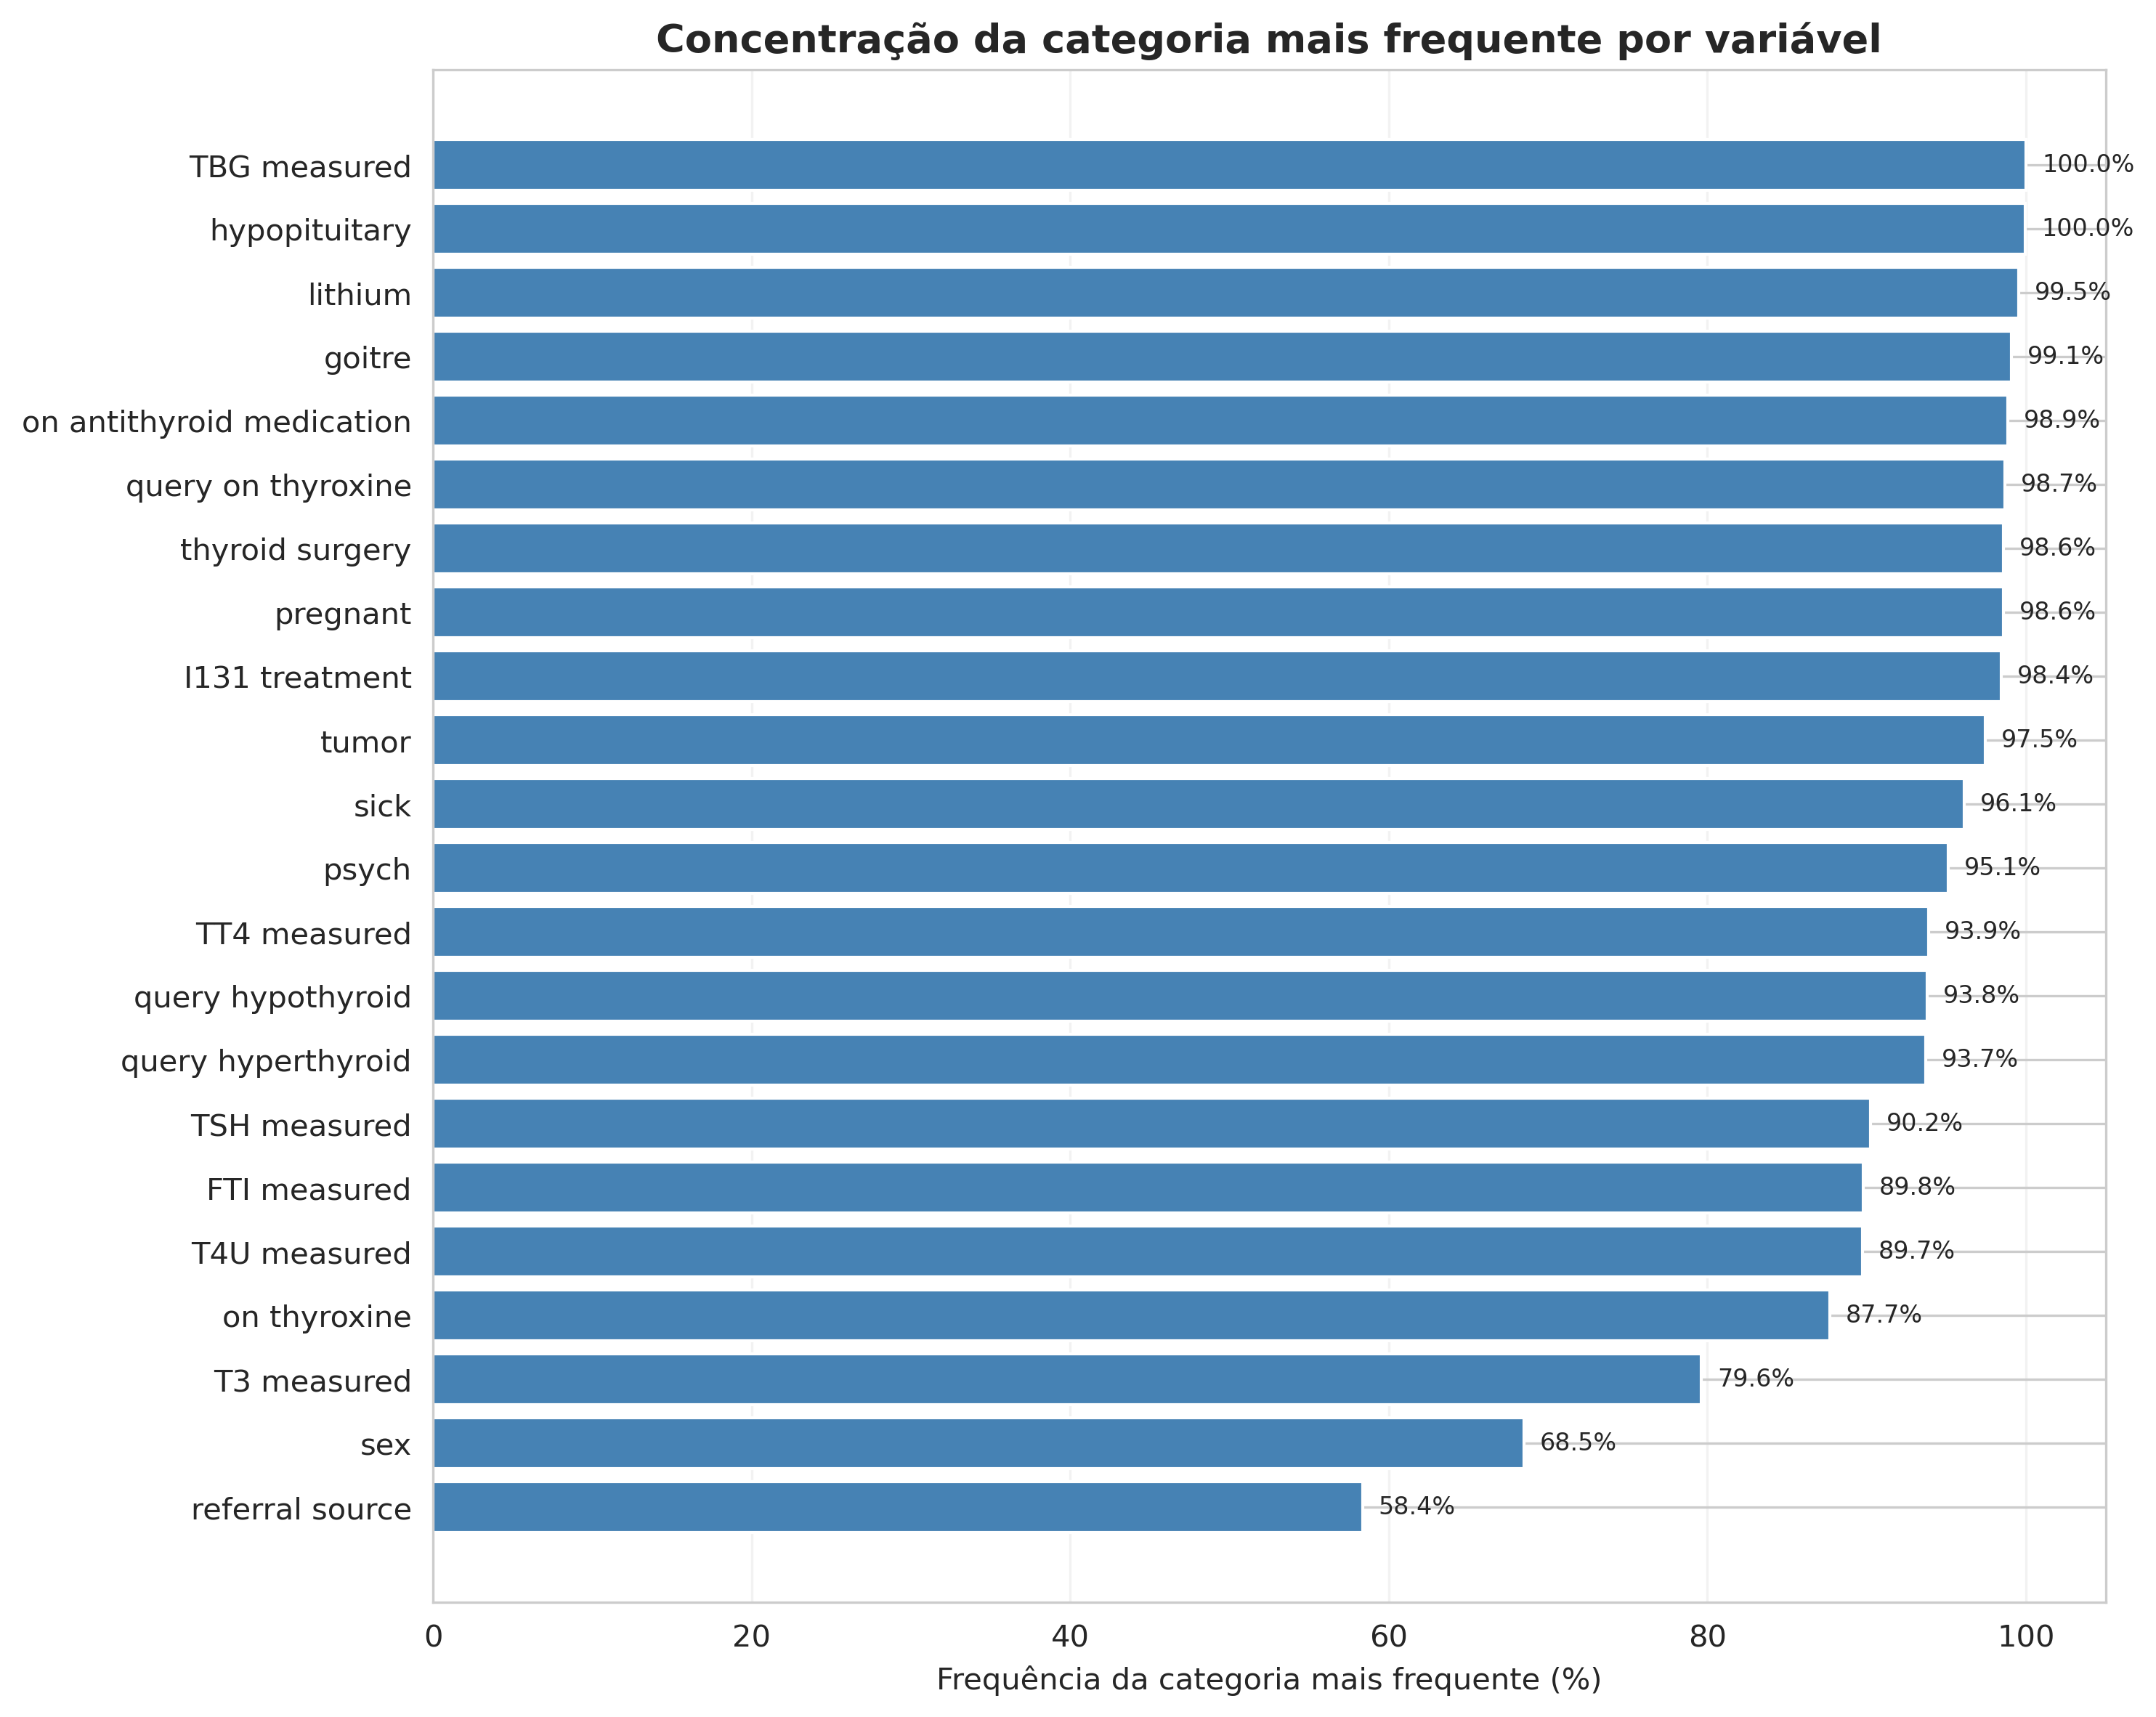
\includegraphics{figuras/eda_12.png}
\caption{Categoria mais frequente}
\end{figure}

\hypertarget{suxedntese-da-anuxe1lise-exploratuxf3ria}{%
\subsubsection{4.7 Síntese da análise
exploratória}\label{suxedntese-da-anuxe1lise-exploratuxf3ria}}

A EDA evidenciou quatro aspectos centrais:

\begin{enumerate}
\def\labelenumi{\arabic{enumi}.}
\tightlist
\item
  \textbf{Desbalanceamento da variável-alvo:} a classe \texttt{N}
  representa apenas 7,71\% dos registros originais.
\item
  \textbf{Qualidade dos dados:} foram identificadas duplicatas exatas,
  uma idade inválida, ausências parciais e uma variável integralmente
  ausente.
\item
  \textbf{Diferenças entre classes:} as medidas laboratoriais,
  especialmente TSH, apresentam diferenças centrais mais expressivas
  entre \texttt{N} e \texttt{P} do que a idade.
\item
  \textbf{Sobreposição entre preditores:} TT4 e FTI apresentam
  correlação positiva elevada, aspecto relevante para a interpretação
  dos modelos.
\end{enumerate}

\hypertarget{preparauxe7uxe3o-dos-dados}{%
\subsection{5. Preparação dos dados}\label{preparauxe7uxe3o-dos-dados}}

A preparação foi realizada antes da modelagem, mantendo a validação
reservada separada durante o desenvolvimento dos modelos.

As operações documentadas foram:

\begin{enumerate}
\def\labelenumi{\arabic{enumi}.}
\tightlist
\item
  conversão das variáveis numéricas;
\item
  tratamento do valor inválido de idade;
\item
  remoção de \texttt{TBG} e \texttt{TBG\ measured};
\item
  codificação do alvo (\texttt{P\ =\ 0}, \texttt{N\ =\ 1});
\item
  remoção das 61 duplicatas excedentes;
\item
  divisão estratificada em 80\% para treinamento e 20\% para validação
  reservada.
\end{enumerate}

Após a preparação, a base analítica passou a conter \textbf{3.711
registros e 28 colunas}. A divisão resultou em:

\begin{longtable}[]{@{}
  >{\raggedright\arraybackslash}p{(\columnwidth - 4\tabcolsep) * \real{0.29}}
  >{\raggedleft\arraybackslash}p{(\columnwidth - 4\tabcolsep) * \real{0.39}}
  >{\raggedright\arraybackslash}p{(\columnwidth - 4\tabcolsep) * \real{0.29}}@{}}
\toprule
Conjunto & Registros & Utilização \\
\midrule
\endhead
Treinamento & 2.968 & Ajuste dos pipelines, validação cruzada e seleção
dos modelos \\
Validação reservada & 743 & Avaliação final dos modelos finalistas \\
\textbf{Total} & \textbf{3.711} & \\
\bottomrule
\end{longtable}

A variável constante \texttt{hypopituitary} foi identificada no conjunto
de treinamento e removida dos preditores utilizados pelos modelos. Com
isso, foram considerados 26 preditores na etapa de modelagem.

\hypertarget{pruxe9-processamento-integrado-aos-modelos}{%
\subsubsection{5.1 Pré-processamento integrado aos
modelos}\label{pruxe9-processamento-integrado-aos-modelos}}

O pré-processamento foi incorporado aos pipelines para que os
transformadores fossem ajustados somente nos dados de treinamento de
cada fold:

\begin{itemize}
\tightlist
\item
  \textbf{Variáveis numéricas:} imputação pela mediana e padronização
  com \texttt{StandardScaler}.
\item
  \textbf{Variáveis binárias:} imputação pela moda e codificação dos
  valores \texttt{t} e \texttt{f}.
\item
  \textbf{Variáveis categóricas:} imputação pela moda e codificação
  One-Hot, com \texttt{handle\_unknown="ignore"}.
\end{itemize}

Essa organização evita que as estatísticas de imputação, os parâmetros
de padronização ou as categorias observadas na validação de cada fold
sejam utilizados durante o ajuste correspondente.

\hypertarget{estratuxe9gia-de-modelagem-e-avaliauxe7uxe3o}{%
\subsection{6. Estratégia de modelagem e
avaliação}\label{estratuxe9gia-de-modelagem-e-avaliauxe7uxe3o}}

Foram comparados quatro classificadores:

\begin{itemize}
\tightlist
\item
  \textbf{Dummy Classifier:} referência mínima para comparação;
\item
  \textbf{Regressão Logística:} modelo linear de classificação;
\item
  \textbf{Random Forest:} método de ensemble baseado em árvores de
  decisão;
\item
  \textbf{XGBoost:} método de boosting baseado em árvores.
\end{itemize}

A avaliação foi realizada por validação cruzada estratificada, com cinco
folds, embaralhamento e \texttt{random\_state=42}. Os mesmos folds foram
utilizados para comparar os algoritmos.

As métricas adotadas foram:

\begin{itemize}
\tightlist
\item
  \textbf{Precision:} proporção de predições positivas que correspondem
  à classe positiva real;
\item
  \textbf{Recall:} proporção dos registros positivos reais identificados
  pelo modelo;
\item
  \textbf{F1:} média harmônica entre Precision e Recall;
\item
  \textbf{PR-AUC:} área sob a curva Precision-Recall;
\item
  \textbf{ROC-AUC:} área sob a curva ROC.
\end{itemize}

Como \texttt{N} foi definida como classe positiva e é minoritária,
Precision, Recall, F1 e PR-AUC receberam atenção especial na comparação.

\hypertarget{resultados-da-validauxe7uxe3o-cruzada}{%
\subsection{7. Resultados da validação
cruzada}\label{resultados-da-validauxe7uxe3o-cruzada}}

A comparação dos modelos mostrou desempenho elevado para XGBoost e
Random Forest. A Regressão Logística apresentou resultados inferiores,
mas superiores ao baseline em todas as métricas preditivas consideradas.
O Dummy Classifier não apresentou capacidade discriminativa para a
classe positiva.

\begin{longtable}[]{@{}lrrrrr@{}}
\toprule
Modelo & Precision & Recall & F1 & PR-AUC & ROC-AUC \\
\midrule
\endhead
Dummy & 0,000 & 0,000 & 0,000 & 0,079 & 0,500 \\
Regressão Logística & 0,723 & 0,940 & 0,817 & 0,875 & 0,989 \\
Random Forest & 0,926 & 0,991 & 0,957 & 0,990 & 0,999 \\
XGBoost & 0,958 & 0,974 & 0,966 & 0,976 & 0,996 \\
\bottomrule
\end{longtable}

\textbf{Figura 12 --- Comparação das métricas dos modelos na validação
cruzada.}

\begin{figure}
\centering
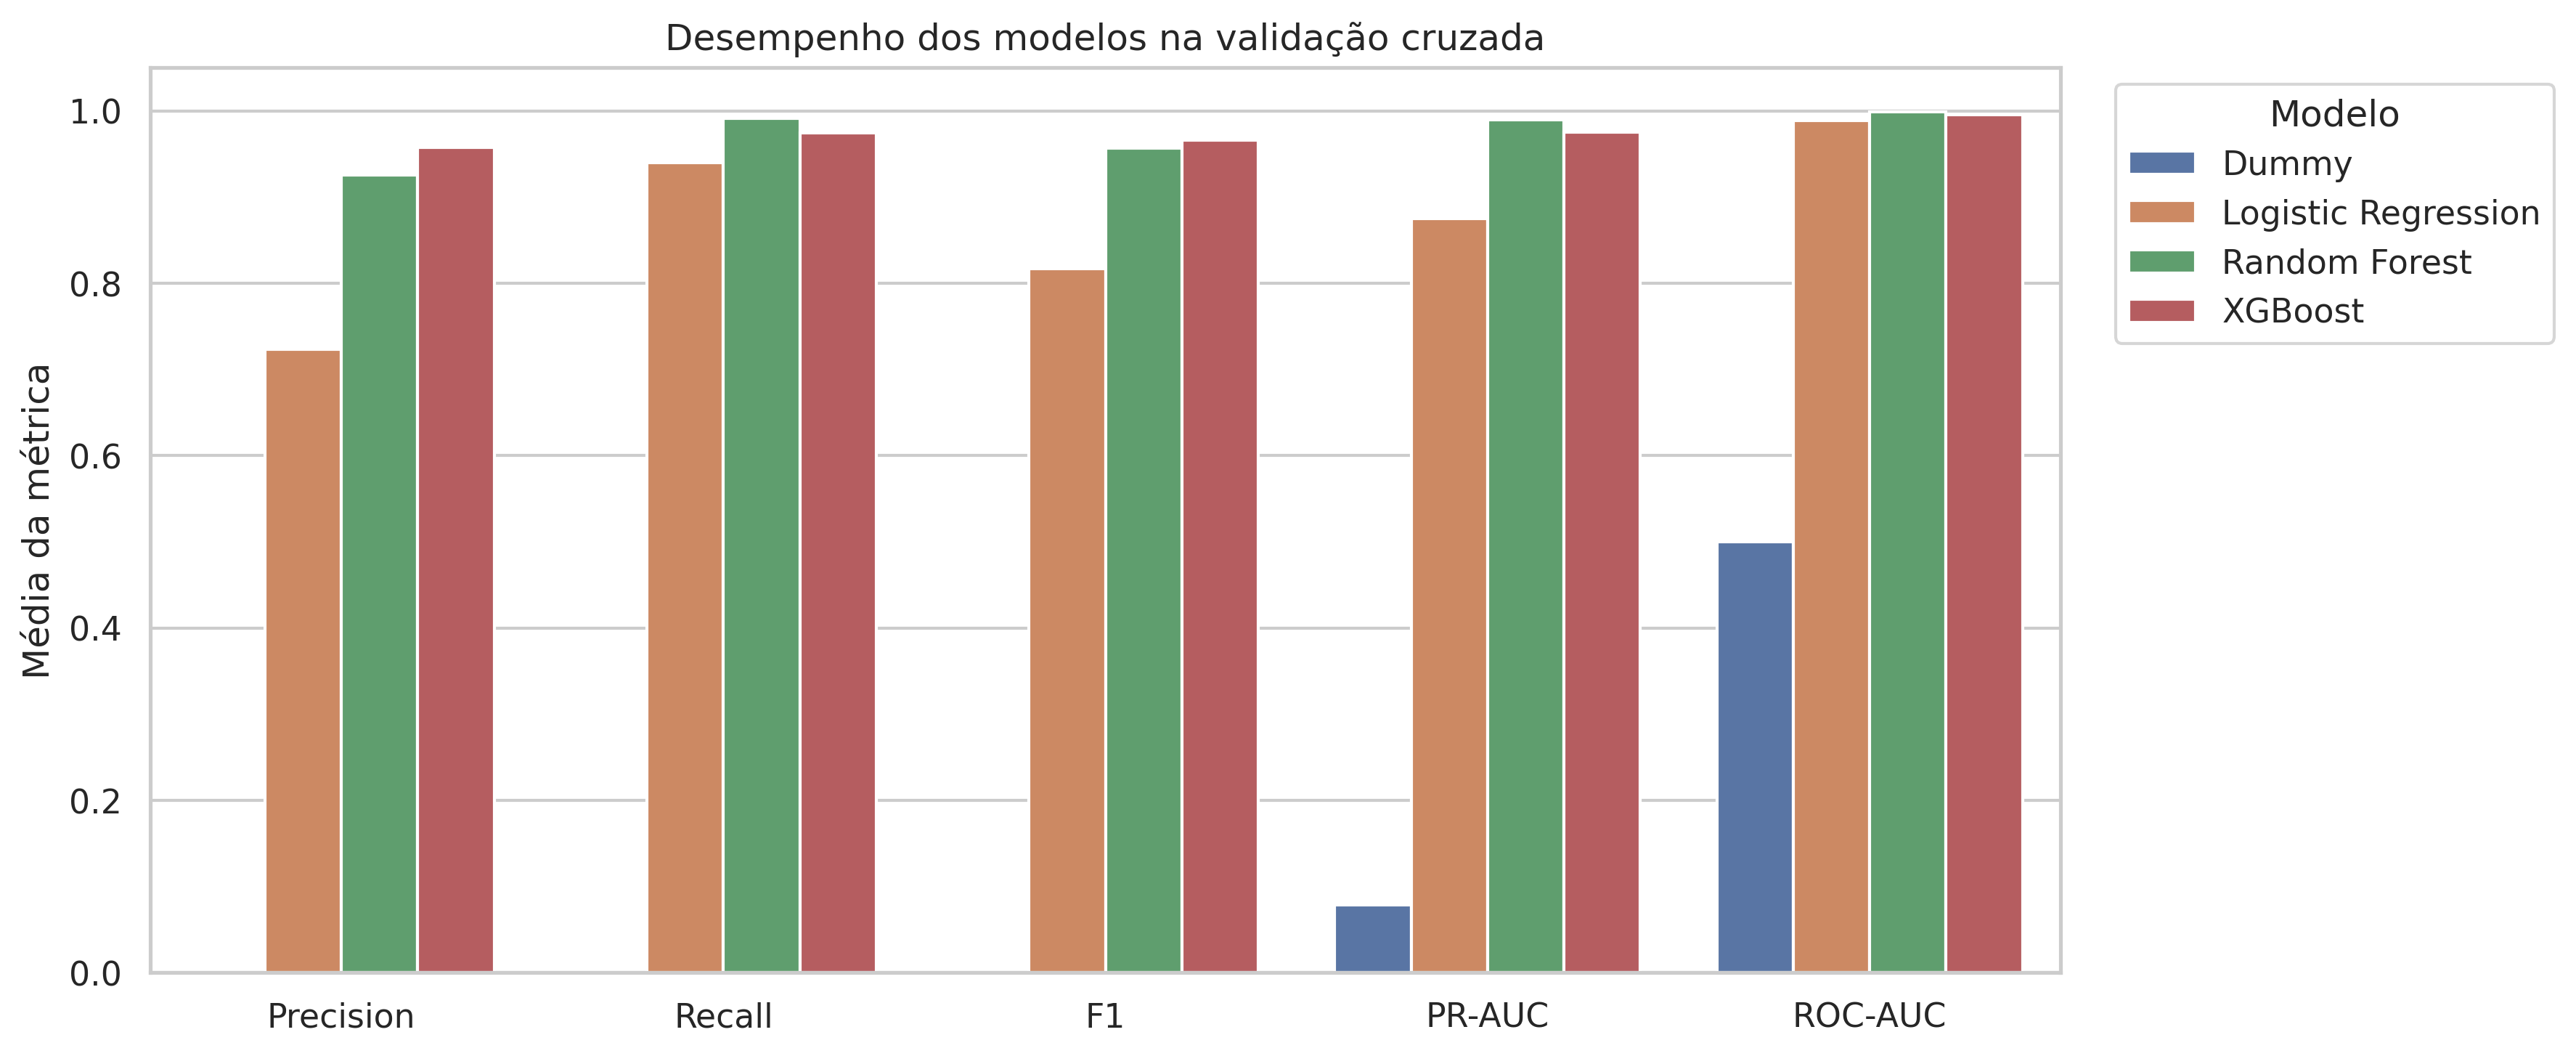
\includegraphics{figuras/ml_01.png}
\caption{Métricas da validação cruzada}
\end{figure}

O XGBoost apresentou o maior F1 médio (0,966), enquanto o Random Forest
obteve o maior Recall (0,991), PR-AUC (0,990) e ROC-AUC (0,999). Os dois
modelos foram mantidos como finalistas por apresentarem desempenho
elevado e características complementares.

\hypertarget{interpretauxe7uxe3o-dos-modelos}{%
\subsection{8. Interpretação dos
modelos}\label{interpretauxe7uxe3o-dos-modelos}}

\hypertarget{importuxe2ncia-por-permutauxe7uxe3o}{%
\subsubsection{8.1 Importância por
permutação}\label{importuxe2ncia-por-permutauxe7uxe3o}}

A importância por permutação foi calculada nos folds internos do
treinamento. Em cada fold, o pipeline foi ajustado na parcela de
treinamento e a importância foi avaliada na parcela de validação
correspondente. O conjunto reservado permaneceu intocado.

O TSH apresentou a maior importância entre os preditores nos três
modelos preditivos: 0,796 no XGBoost, 0,767 no Random Forest e 0,687 na
Regressão Logística. A variável \texttt{on\ thyroxine} ocupou a segunda
posição nos três modelos. \texttt{thyroid\ surgery} apresentou maior
relevância nos modelos baseados em árvores, enquanto TT4 e T4U
demonstraram maior importância relativa na Regressão Logística.

\textbf{Figura 13 --- Importância por permutação dos preditores nos
modelos.}

\begin{figure}
\centering
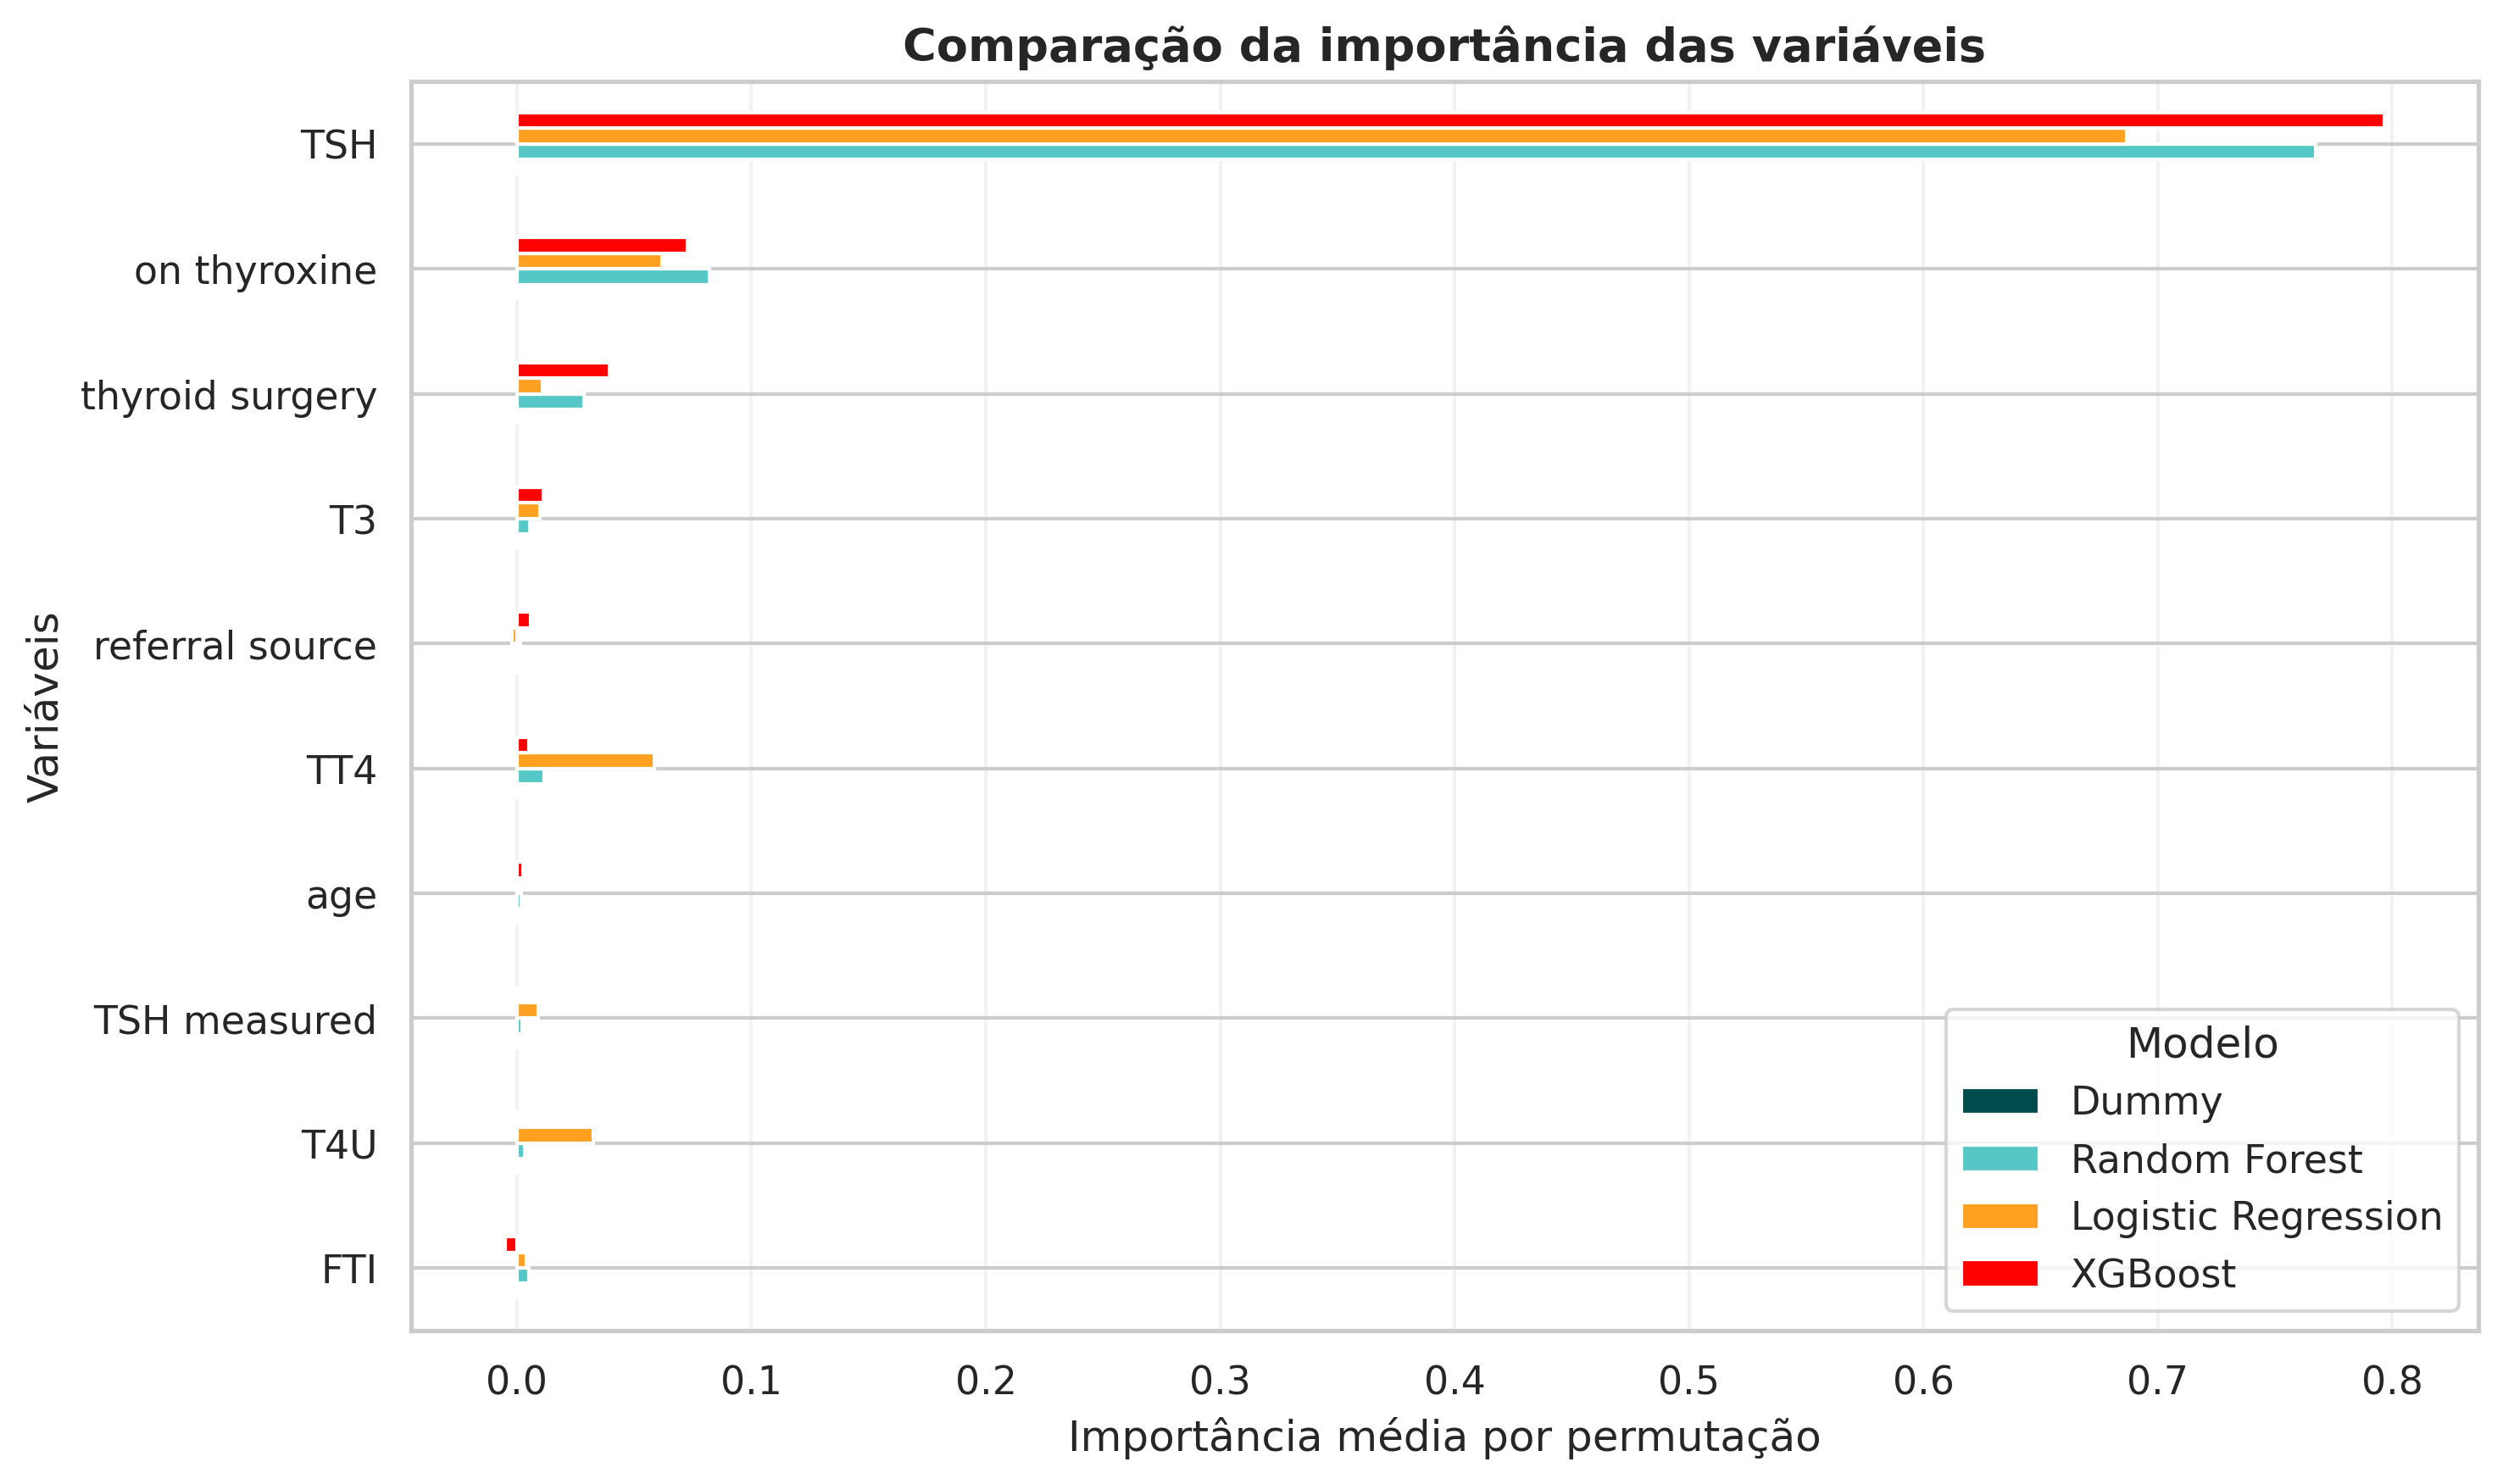
\includegraphics{figuras/ml_02.png}
\caption{Importância por permutação}
\end{figure}

A convergência dos modelos quanto à predominância do TSH motivou um
experimento de sensibilidade. A importância por permutação representa
contribuição preditiva no contexto do modelo e dos dados utilizados; não
representa efeito causal ou relevância clínica independente.

\hypertarget{anuxe1lise-de-sensibilidade-sem-tsh}{%
\subsubsection{8.2 Análise de sensibilidade sem
TSH}\label{anuxe1lise-de-sensibilidade-sem-tsh}}

Foi realizado um experimento retirando a variável \texttt{TSH} e
mantendo os demais preditores e parâmetros. A avaliação continuou
restrita à validação cruzada no conjunto de treinamento.

\begin{longtable}[]{@{}lrrrr@{}}
\toprule
Modelo & F1 com TSH & F1 sem TSH & PR-AUC sem TSH & ROC-AUC sem TSH \\
\midrule
\endhead
Regressão Logística & 0,817 & 0,372 & 0,539 & 0,877 \\
Random Forest & 0,957 & 0,493 & 0,545 & 0,865 \\
XGBoost & 0,966 & 0,439 & 0,558 & 0,867 \\
\bottomrule
\end{longtable}

\textbf{Figura 14 --- Sensibilidade dos modelos à retirada de TSH.}

\begin{figure}
\centering
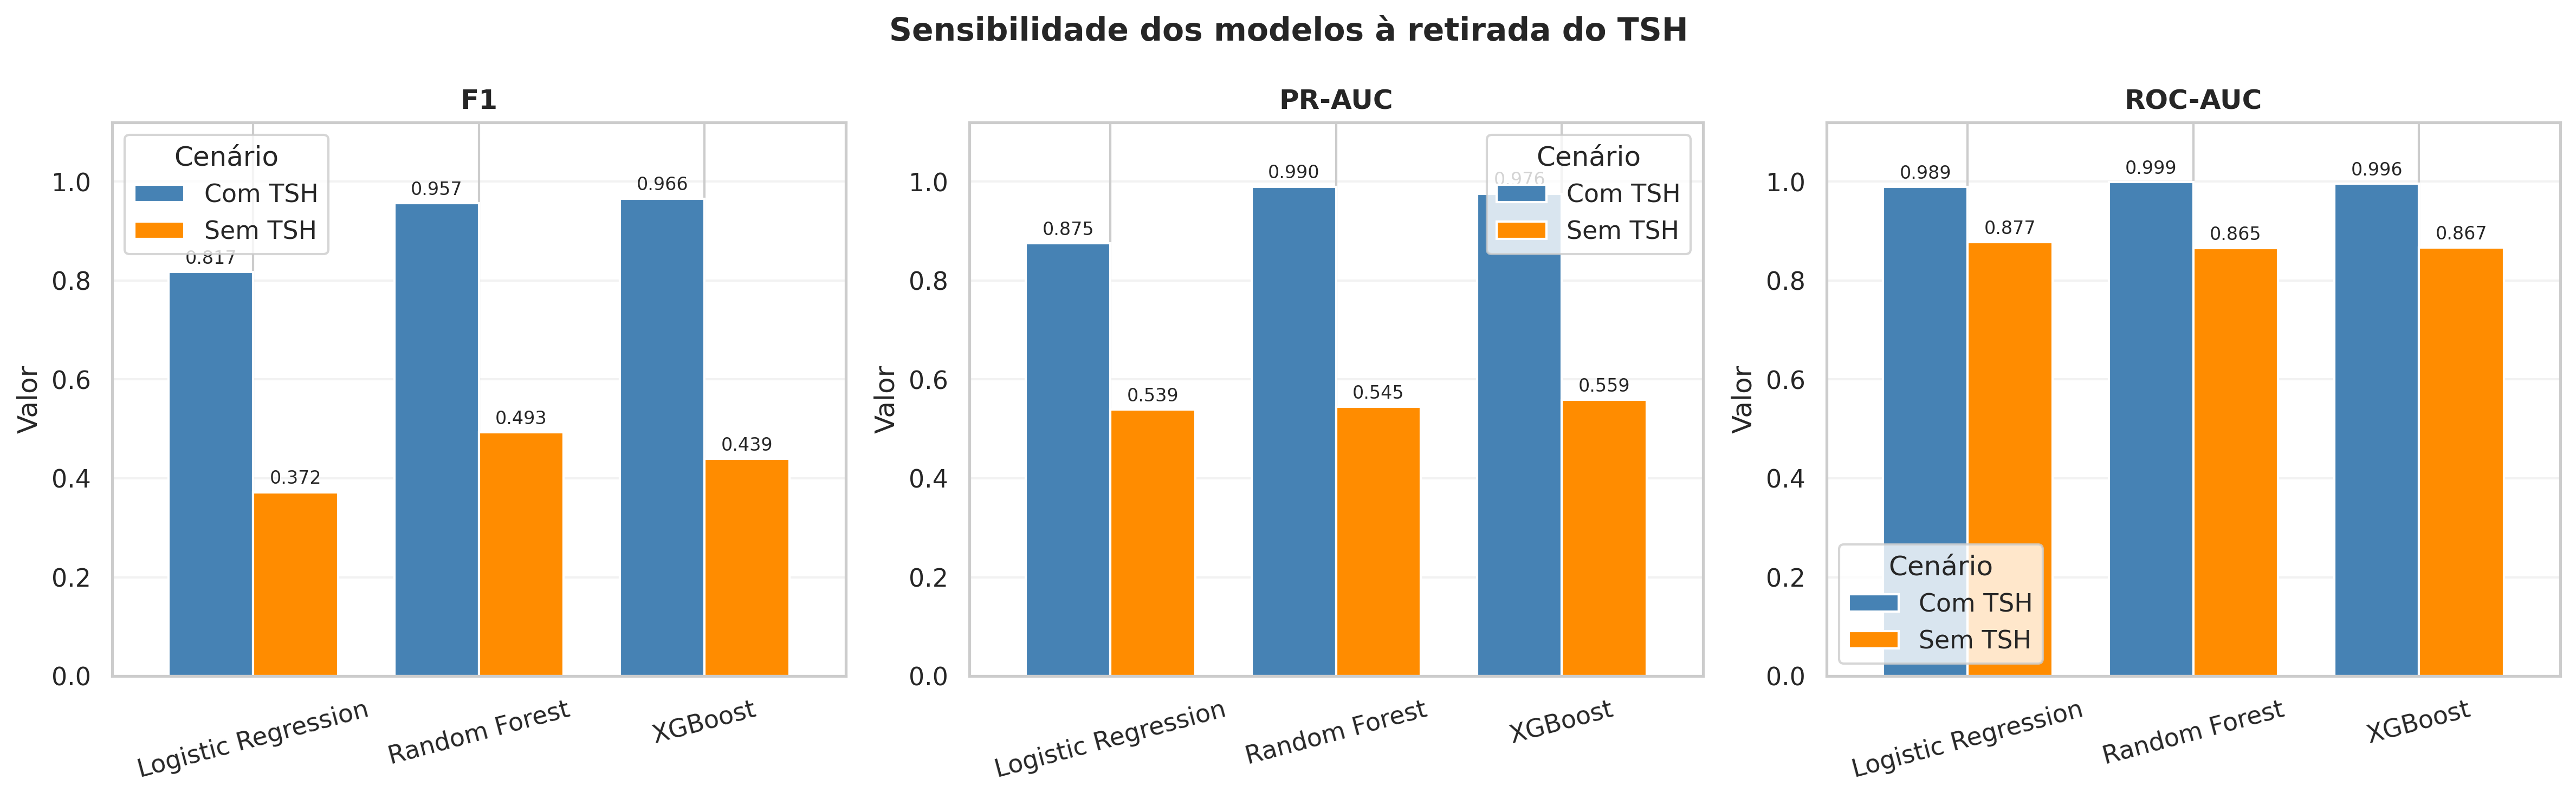
\includegraphics{figuras/ml_03.png}
\caption{Sensibilidade sem TSH}
\end{figure}

A retirada de TSH provocou redução expressiva do desempenho dos três
modelos. O F1 do XGBoost caiu de 0,966 para 0,439; o Random Forest
passou de 0,957 para 0,493; e a Regressão Logística, de 0,817 para
0,372.

A PR-AUC também apresentou queda acentuada. No cenário sem TSH, os
valores ficaram entre 0,539 e 0,558, indicando perda importante da
capacidade de ordenação dos registros positivos.

\hypertarget{importuxe2ncia-das-variuxe1veis-sem-tsh}{%
\subsubsection{8.3 Importância das variáveis sem
TSH}\label{importuxe2ncia-das-variuxe1veis-sem-tsh}}

Após a retirada de TSH, a contribuição preditiva foi redistribuída entre
os demais atributos. TT4, FTI e T3 passaram a concentrar as maiores
importâncias nos três modelos avaliados. TT4 apresentou a maior
importância na Regressão Logística e no XGBoost, enquanto FTI ocupou
essa posição no Random Forest, com valor próximo ao de TT4. T3 manteve a
terceira posição nos três modelos.

\textbf{Figura 15 --- Importância por permutação no cenário sem TSH.}

\begin{figure}
\centering
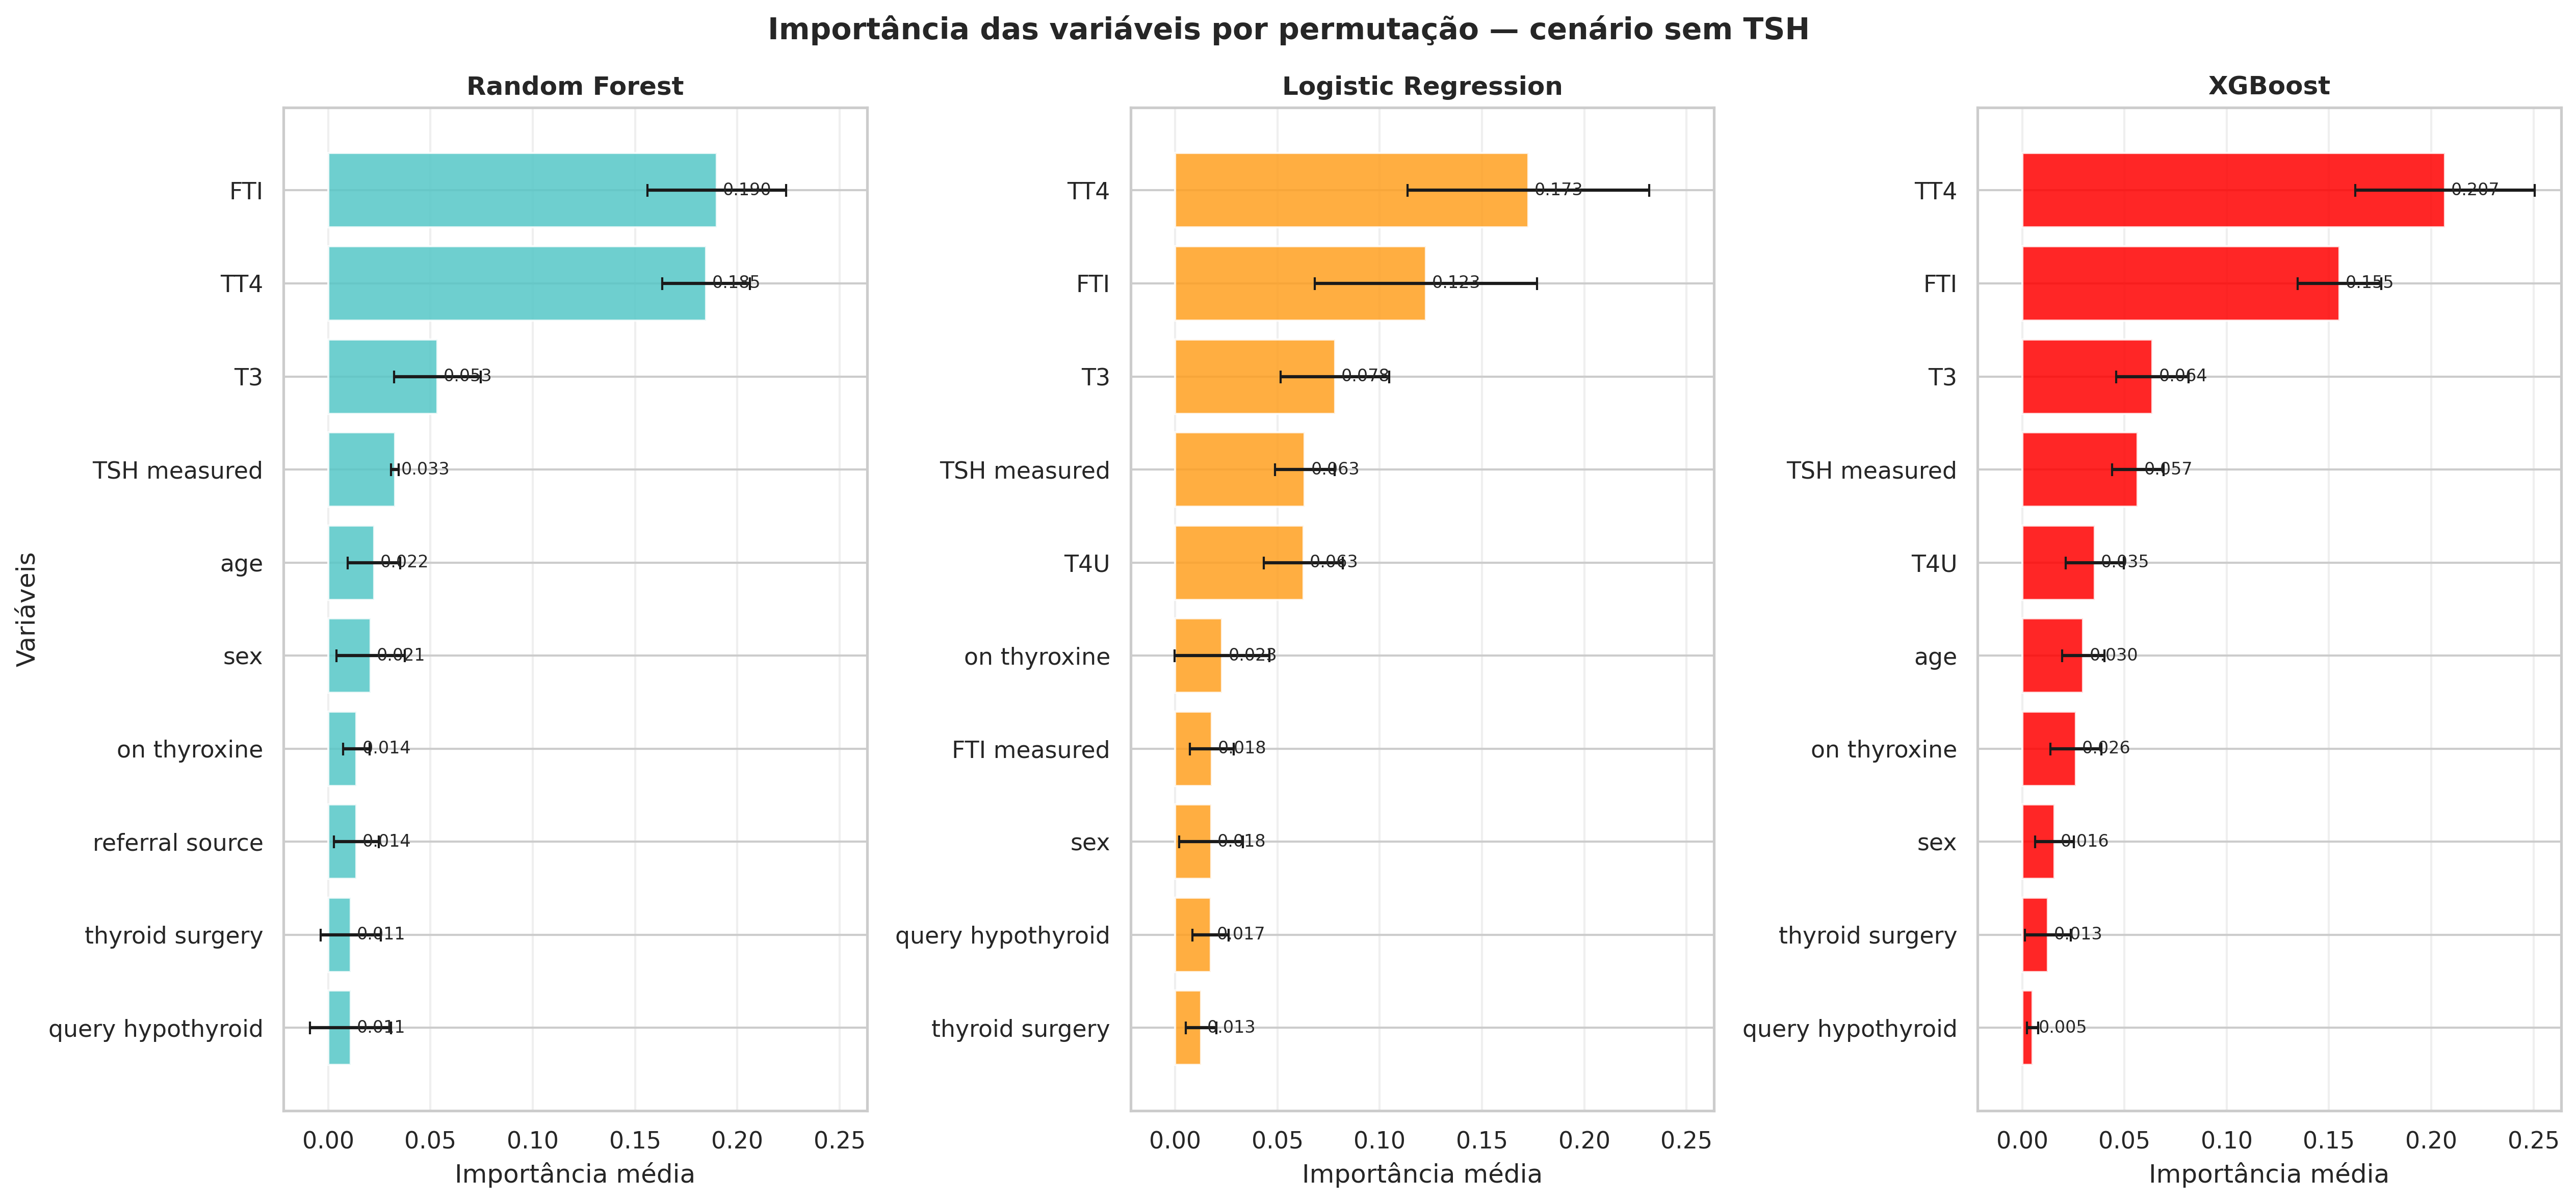
\includegraphics{figuras/ml_04.png}
\caption{Importância sem TSH}
\end{figure}

Apesar da contribuição dos demais indicadores laboratoriais, eles não
compensaram integralmente a retirada de TSH, conforme demonstrado pela
redução das métricas.

\hypertarget{associauxe7uxe3o-entre-variuxe1veis-categuxf3ricas-e-a-classe}{%
\subsubsection{8.4 Associação entre variáveis categóricas e a
classe}\label{associauxe7uxe3o-entre-variuxe1veis-categuxf3ricas-e-a-classe}}

A associação entre variáveis categóricas e \texttt{binaryClass} foi
investigada por meio do V de Cramer, acompanhado dos testes estatísticos
correspondentes. \texttt{on\ thyroxine} e \texttt{query\ hypothyroid}
apresentaram evidência estatística de associação com a classe, ambas com
p-valores inferiores a 0,001. Entretanto, os valores de V de Cramer
foram baixos: 0,082 e 0,095, respectivamente.

As variáveis \texttt{thyroid\ surgery}, \texttt{goitre} e
\texttt{TT4\ measured} não apresentaram associação estatisticamente
significativa ao nível de 5\%.

\textbf{Figura 16 --- Associação entre variáveis categóricas e a classe,
medida pelo V de Cramer.}

\begin{figure}
\centering
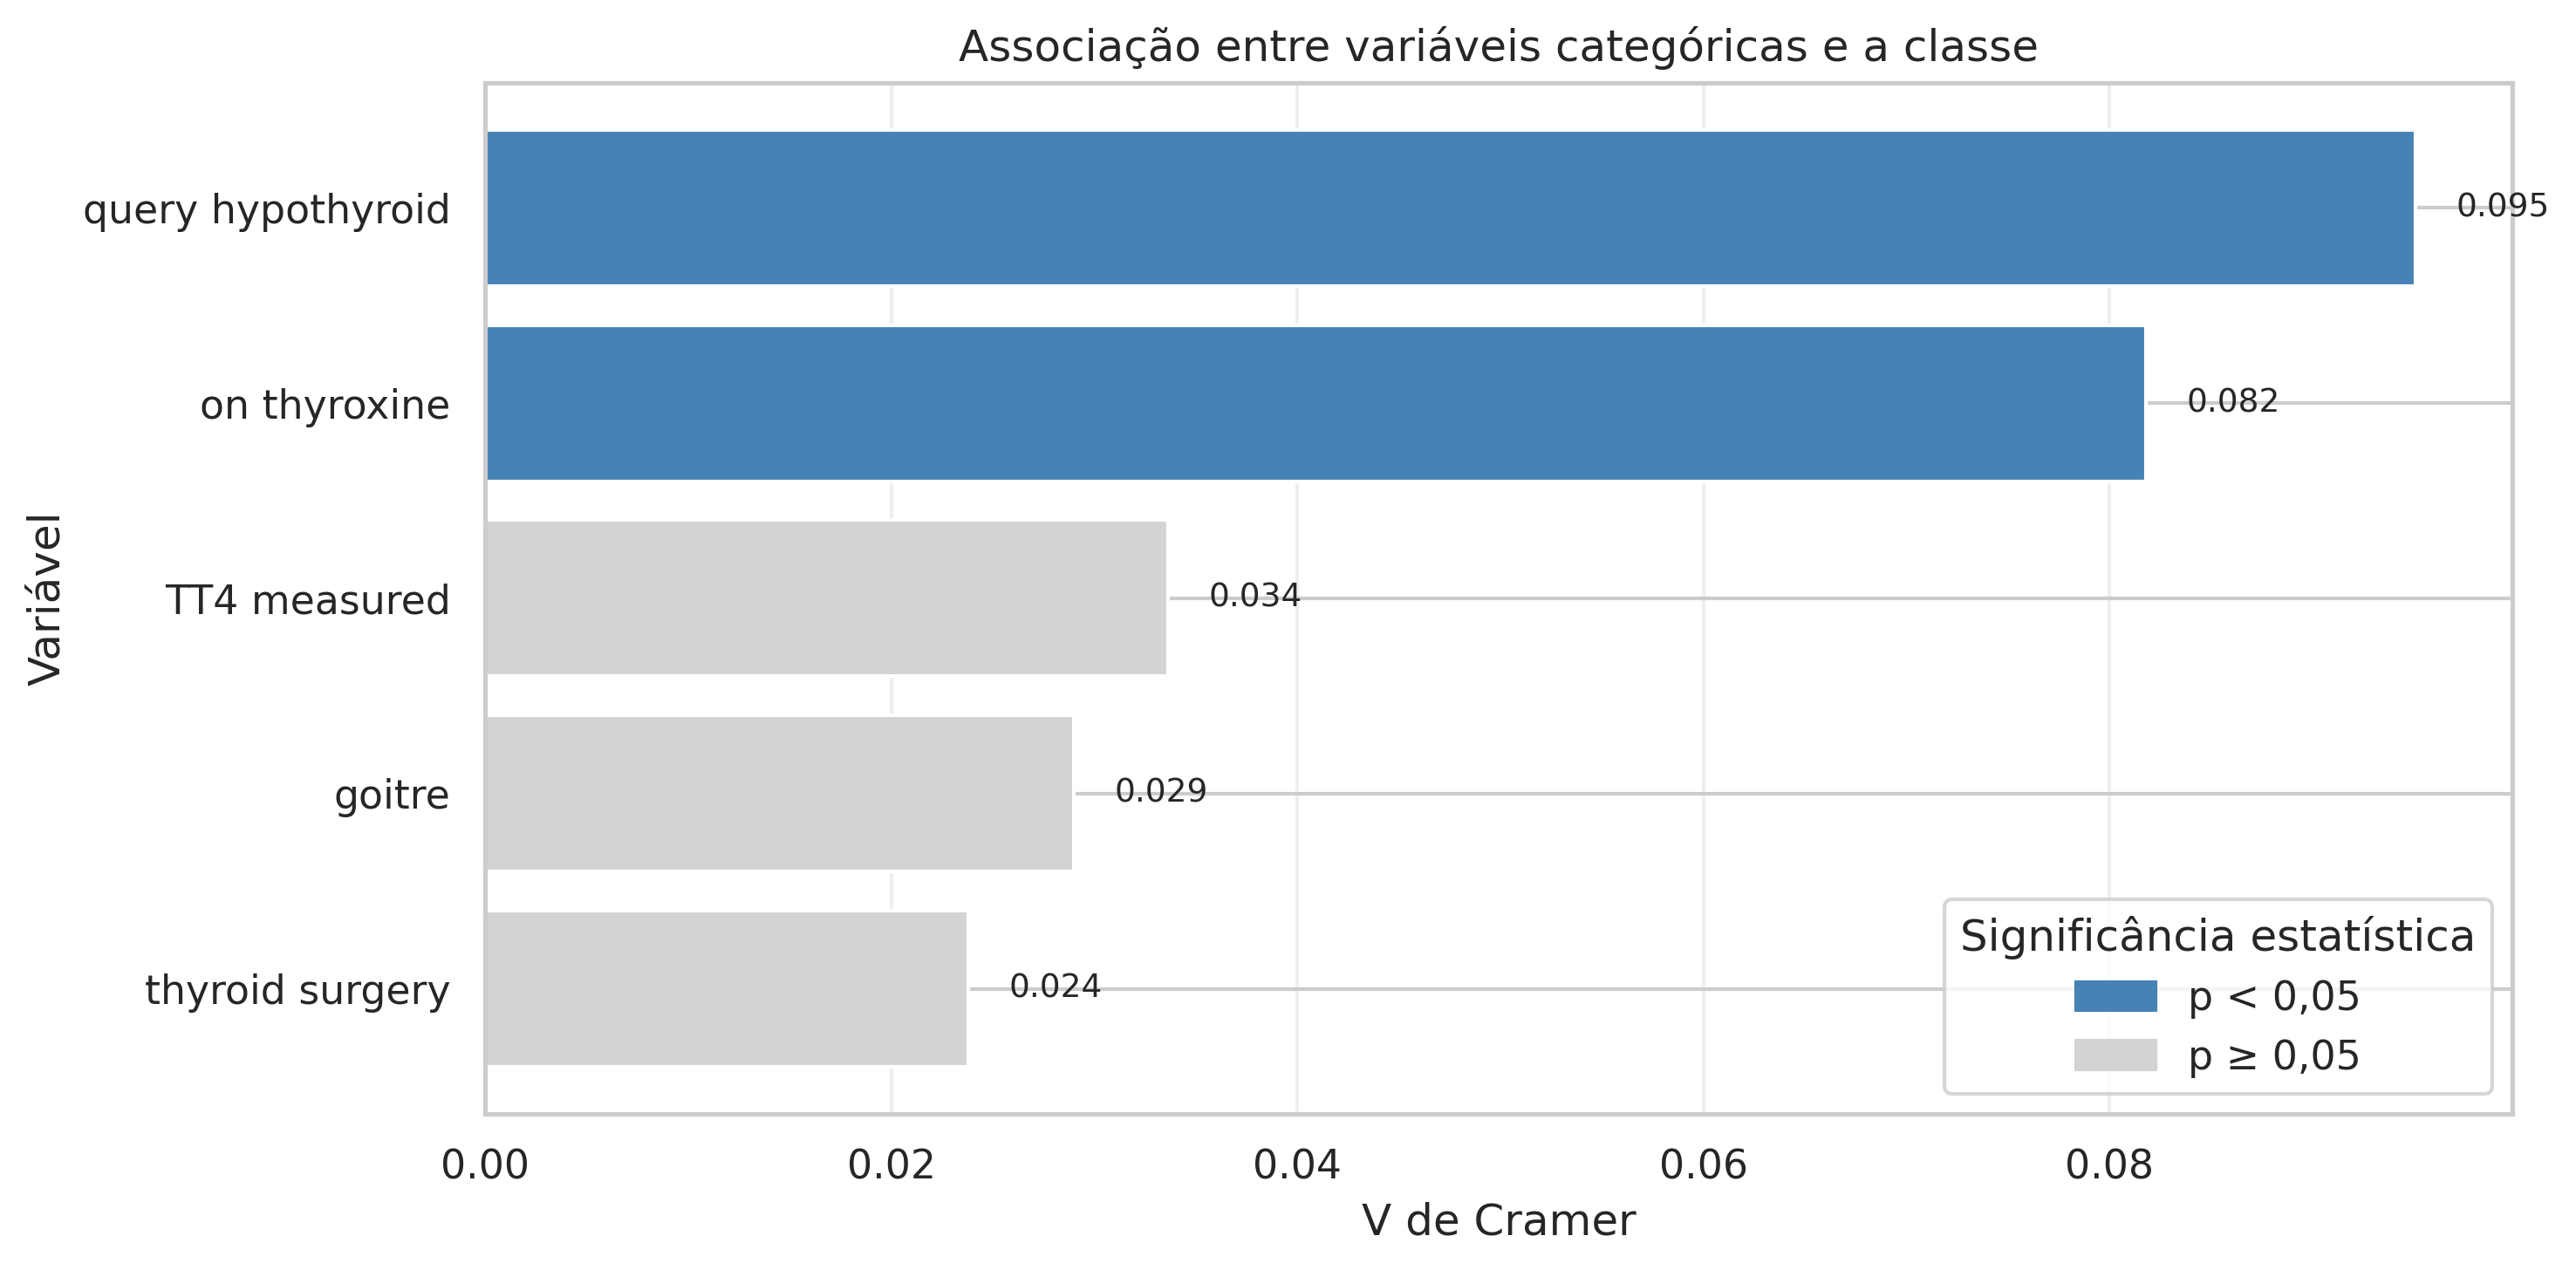
\includegraphics{figuras/ml_05.png}
\caption{V de Cramer}
\end{figure}

A significância estatística não implica associação forte. Os valores de
V de Cramer indicam baixa intensidade nas associações identificadas.

\hypertarget{seleuxe7uxe3o-dos-modelos-finalistas}{%
\subsection{9. Seleção dos modelos
finalistas}\label{seleuxe7uxe3o-dos-modelos-finalistas}}

A seleção foi fundamentada nos resultados da validação cruzada, sem
utilizar o conjunto reservado para orientar escolhas ou ajustes. XGBoost
e Random Forest foram selecionados para a avaliação final.

O XGBoost apresentou maior F1 médio, enquanto o Random Forest obteve
maior Recall e PR-AUC. A manutenção dos dois finalistas permitiu
comparar modelos com características distintas, sem estabelecer
antecipadamente uma superioridade absoluta.

\textbf{Figura 17 --- Comparação dos modelos finalistas na validação
cruzada.}

\begin{figure}
\centering
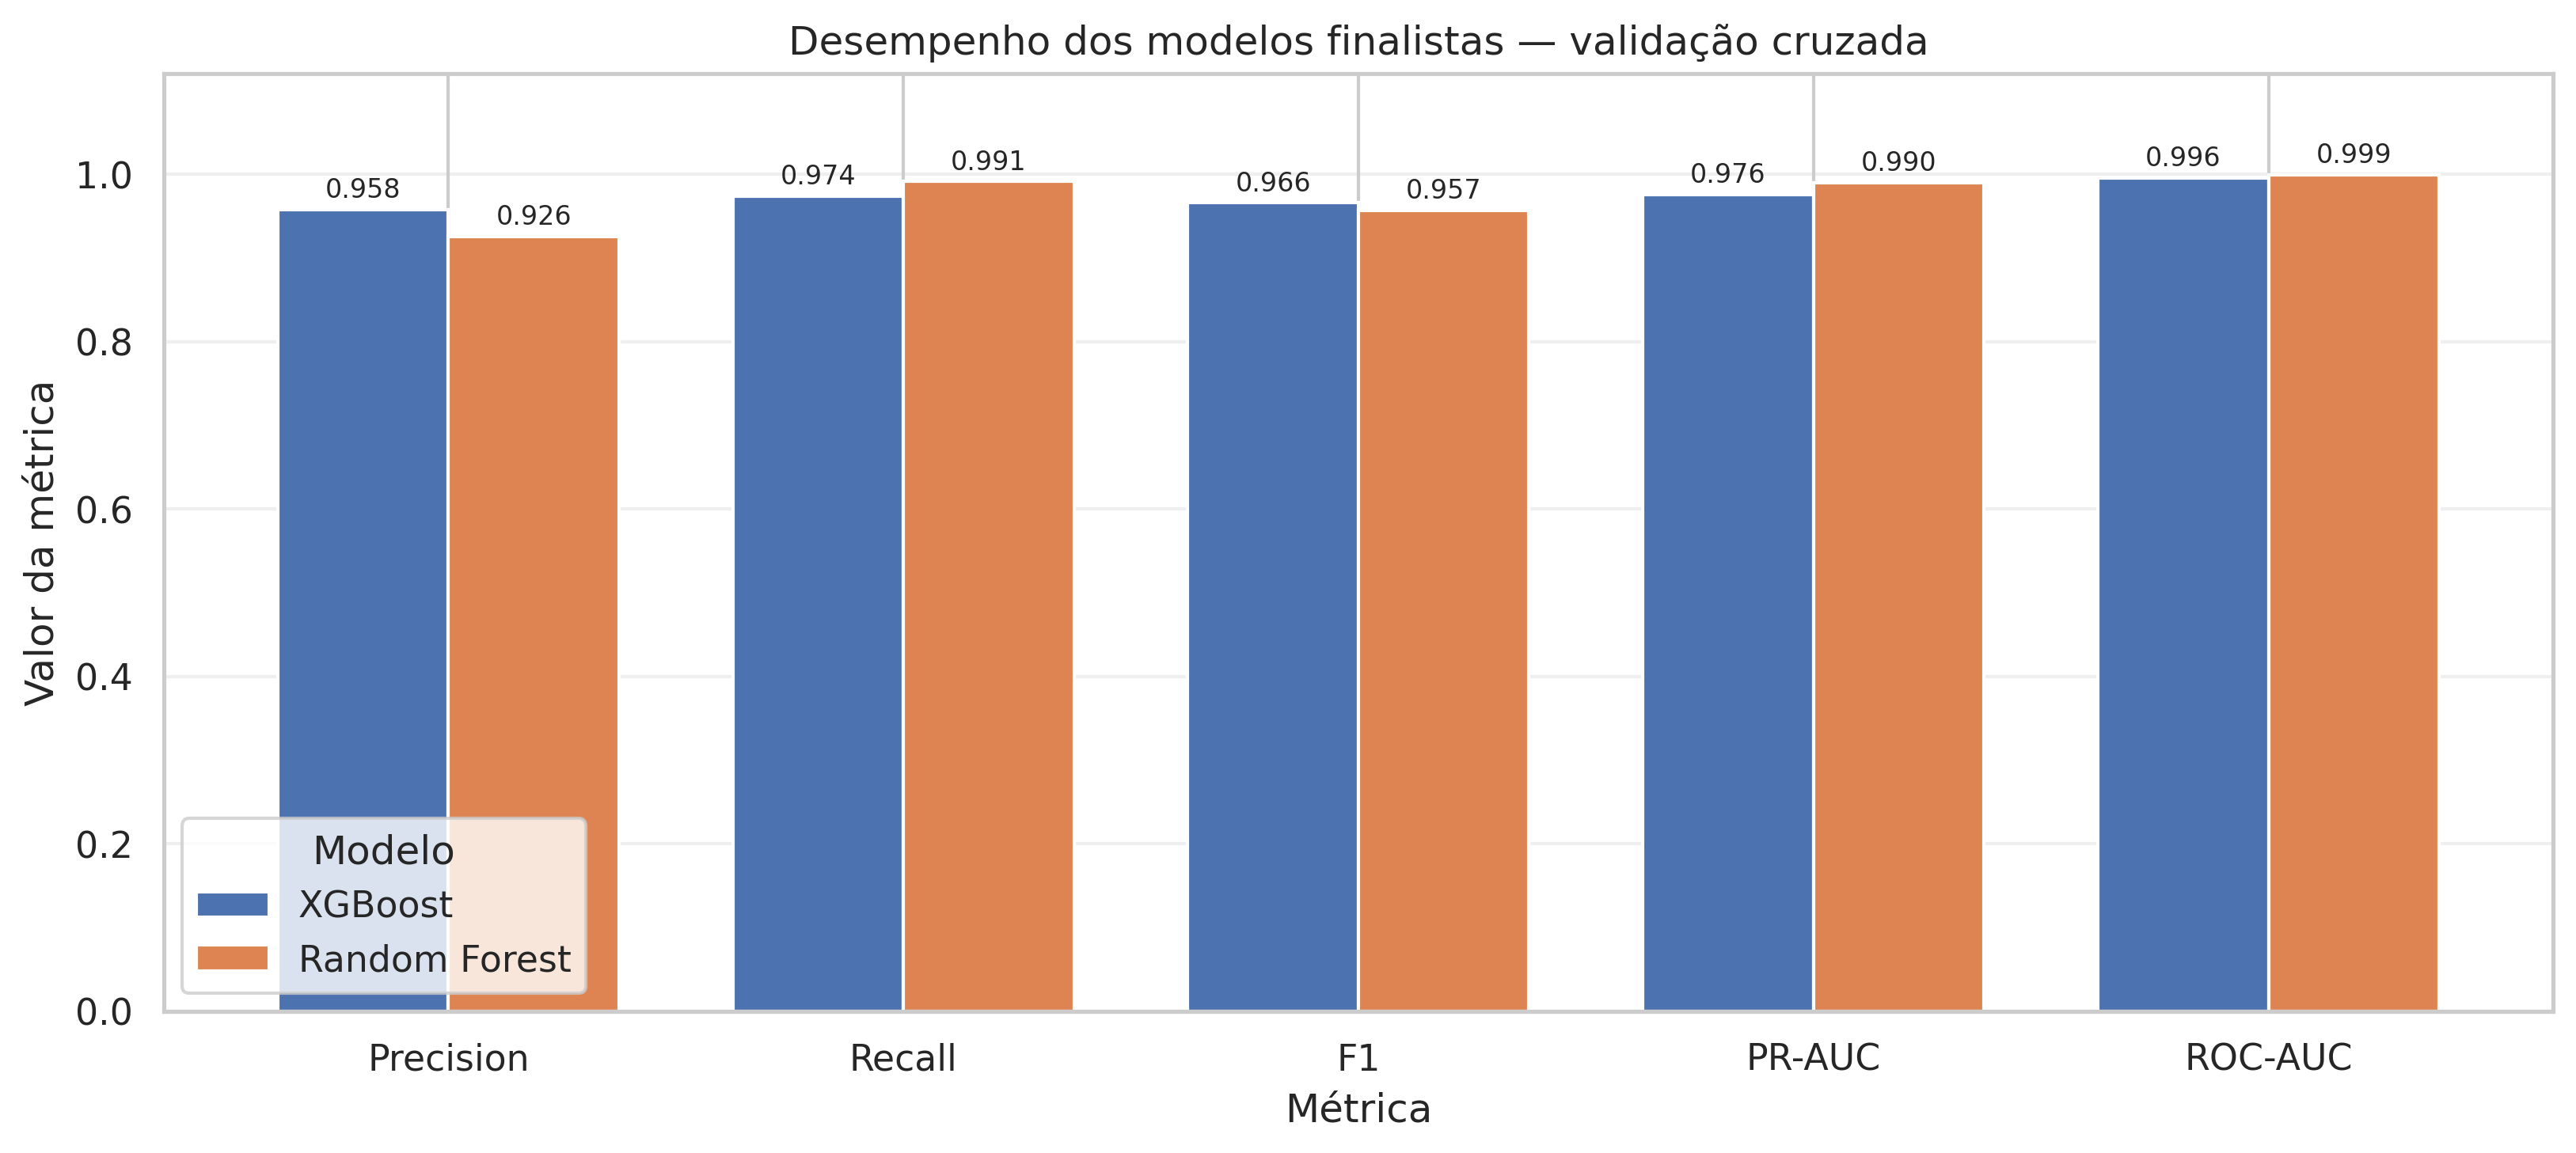
\includegraphics{figuras/ml_06.png}
\caption{Modelos finalistas}
\end{figure}

\hypertarget{avaliauxe7uxe3o-final-na-validauxe7uxe3o-reservada}{%
\subsection{10. Avaliação final na validação
reservada}\label{avaliauxe7uxe3o-final-na-validauxe7uxe3o-reservada}}

Após a seleção, os modelos finalistas foram ajustados com todo o
conjunto de treinamento e avaliados nos 743 registros reservados. Esse
conjunto não participou da validação cruzada, da seleção dos modelos ou
da análise de importância.

\hypertarget{muxe9tricas-finais}{%
\subsubsection{10.1 Métricas finais}\label{muxe9tricas-finais}}

\begin{longtable}[]{@{}lrrrrr@{}}
\toprule
Modelo & Precision & Recall & F1 & PR-AUC & ROC-AUC \\
\midrule
\endhead
XGBoost & 1,000 & 0,983 & 0,991 & 1,000 & 1,000 \\
Random Forest & 0,983 & 1,000 & 0,992 & 1,000 & 1,000 \\
\bottomrule
\end{longtable}

\textbf{Figura 18 --- Métricas dos modelos finalistas na validação
reservada.}

\begin{figure}
\centering
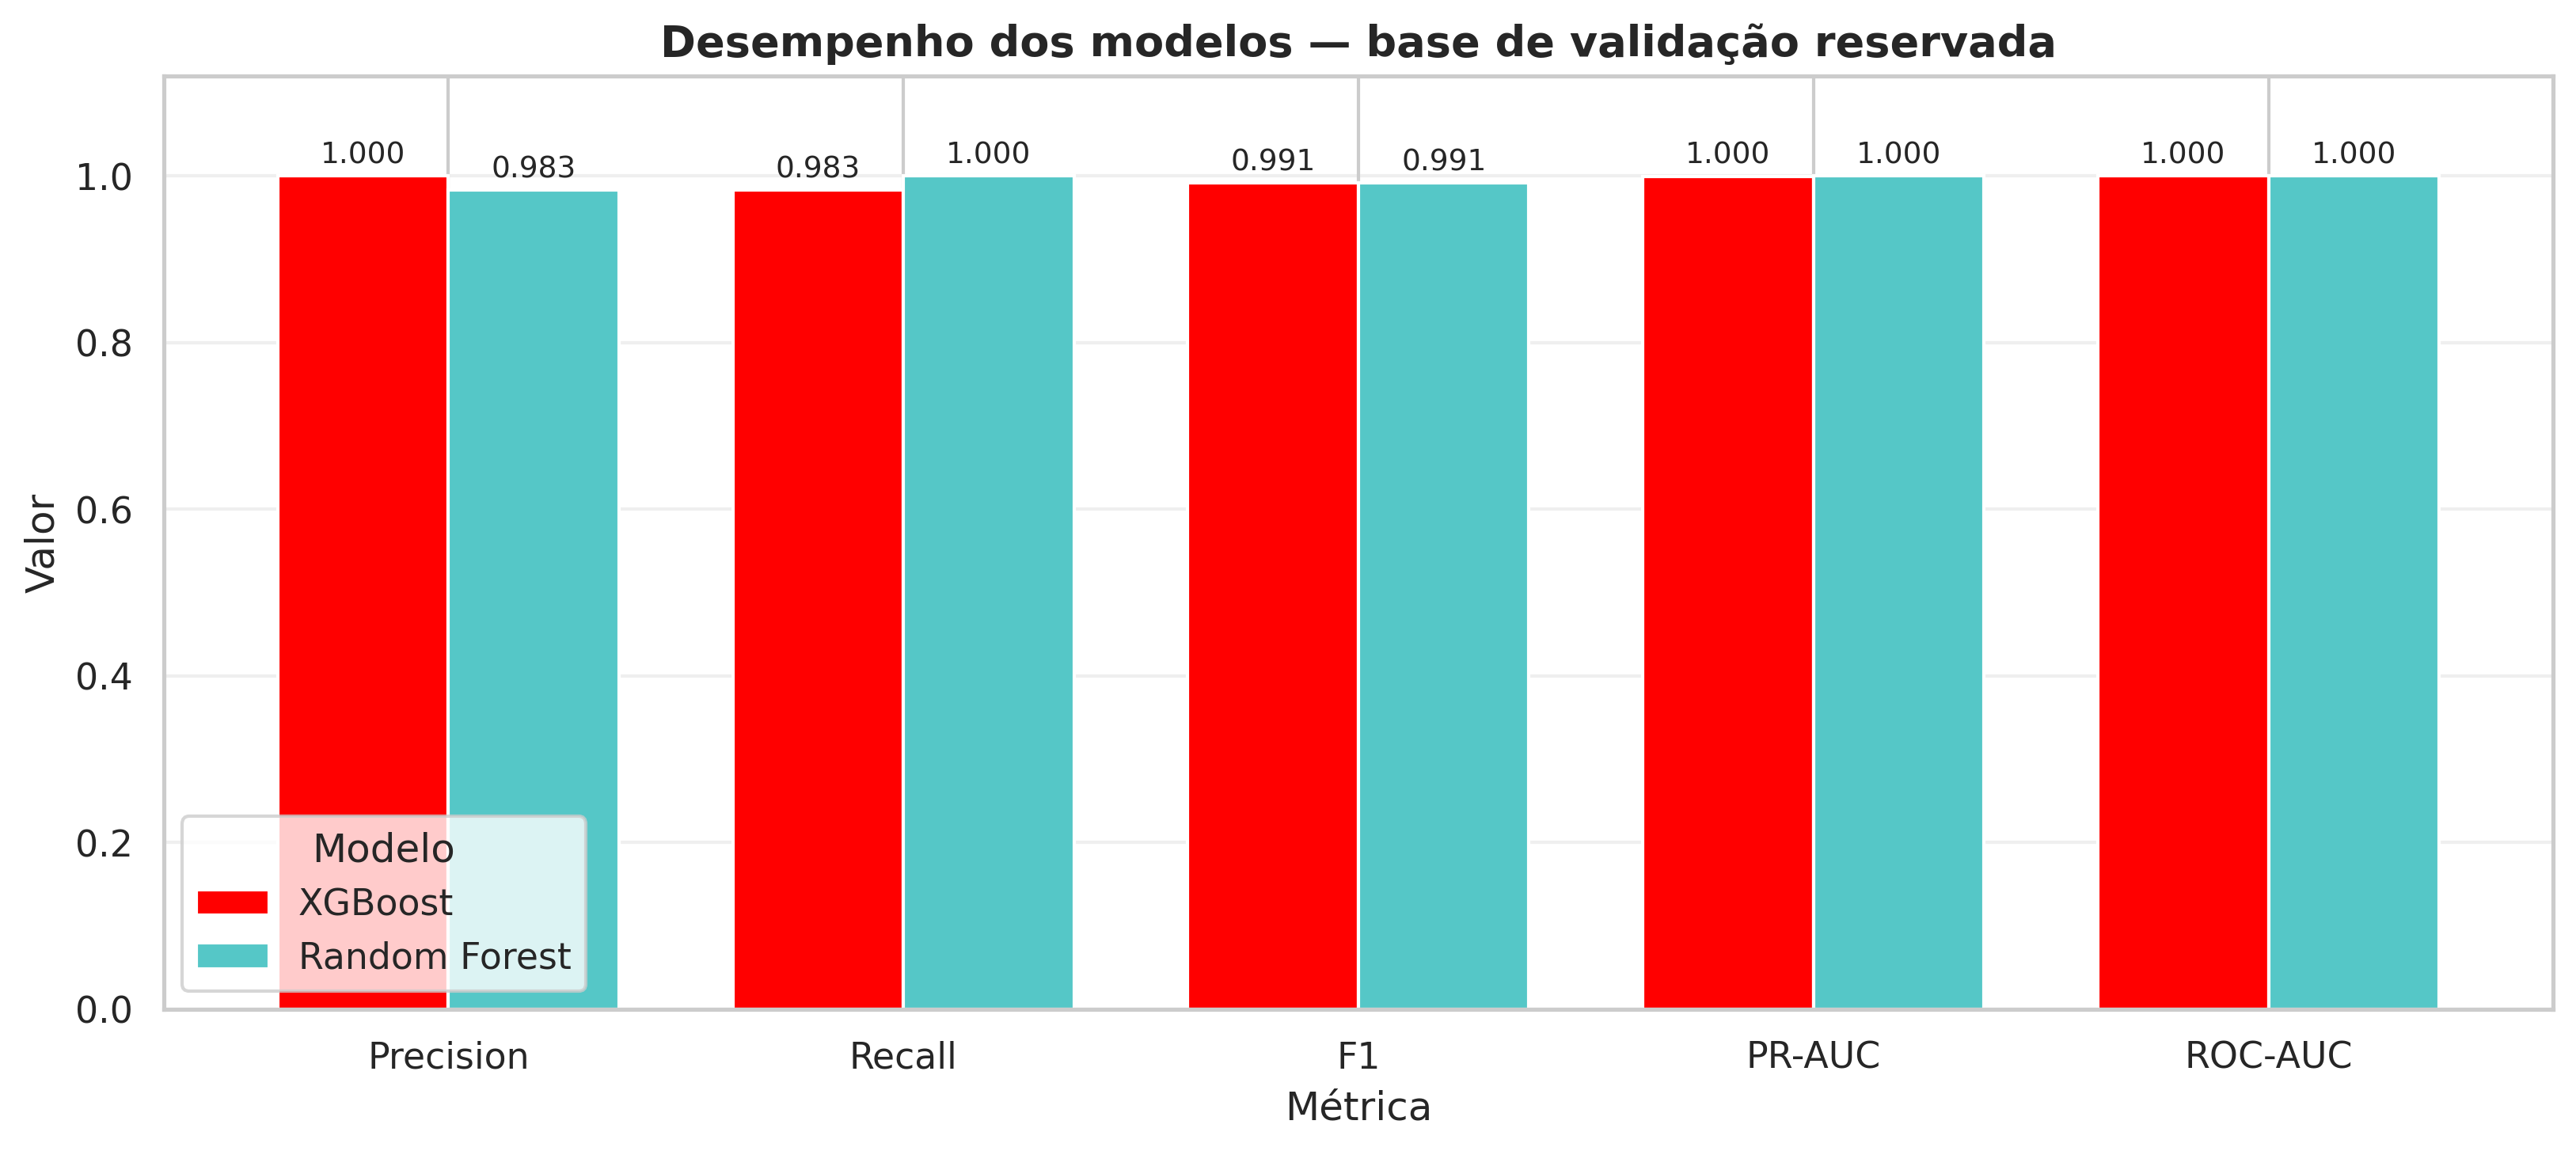
\includegraphics{figuras/ml_08.png}
\caption{Métricas na validação reservada}
\end{figure}

Os dois modelos apresentaram resultados muito próximos. O XGBoost obteve
Precision de 1,000 e Recall de 0,983. O Random Forest alcançou Precision
de 0,983 e Recall de 1,000. Os valores de F1 foram 0,991 e 0,992,
respectivamente.

\hypertarget{matrizes-de-confusuxe3o}{%
\subsubsection{10.2 Matrizes de
confusão}\label{matrizes-de-confusuxe3o}}

As matrizes de confusão permitem observar a distribuição dos erros entre
as classes. Considerando \texttt{N} como classe positiva, os resultados
foram:

\textbf{XGBoost}

\begin{longtable}[]{@{}lrr@{}}
\toprule
Classe real & Predito P & Predito N \\
\midrule
\endhead
P & 685 & 0 \\
N & 1 & 57 \\
\bottomrule
\end{longtable}

\textbf{Random Forest}

\begin{longtable}[]{@{}lrr@{}}
\toprule
Classe real & Predito P & Predito N \\
\midrule
\endhead
P & 684 & 1 \\
N & 0 & 58 \\
\bottomrule
\end{longtable}

\textbf{Figura 19 --- Matrizes de confusão dos modelos finalistas.}

\begin{figure}
\centering
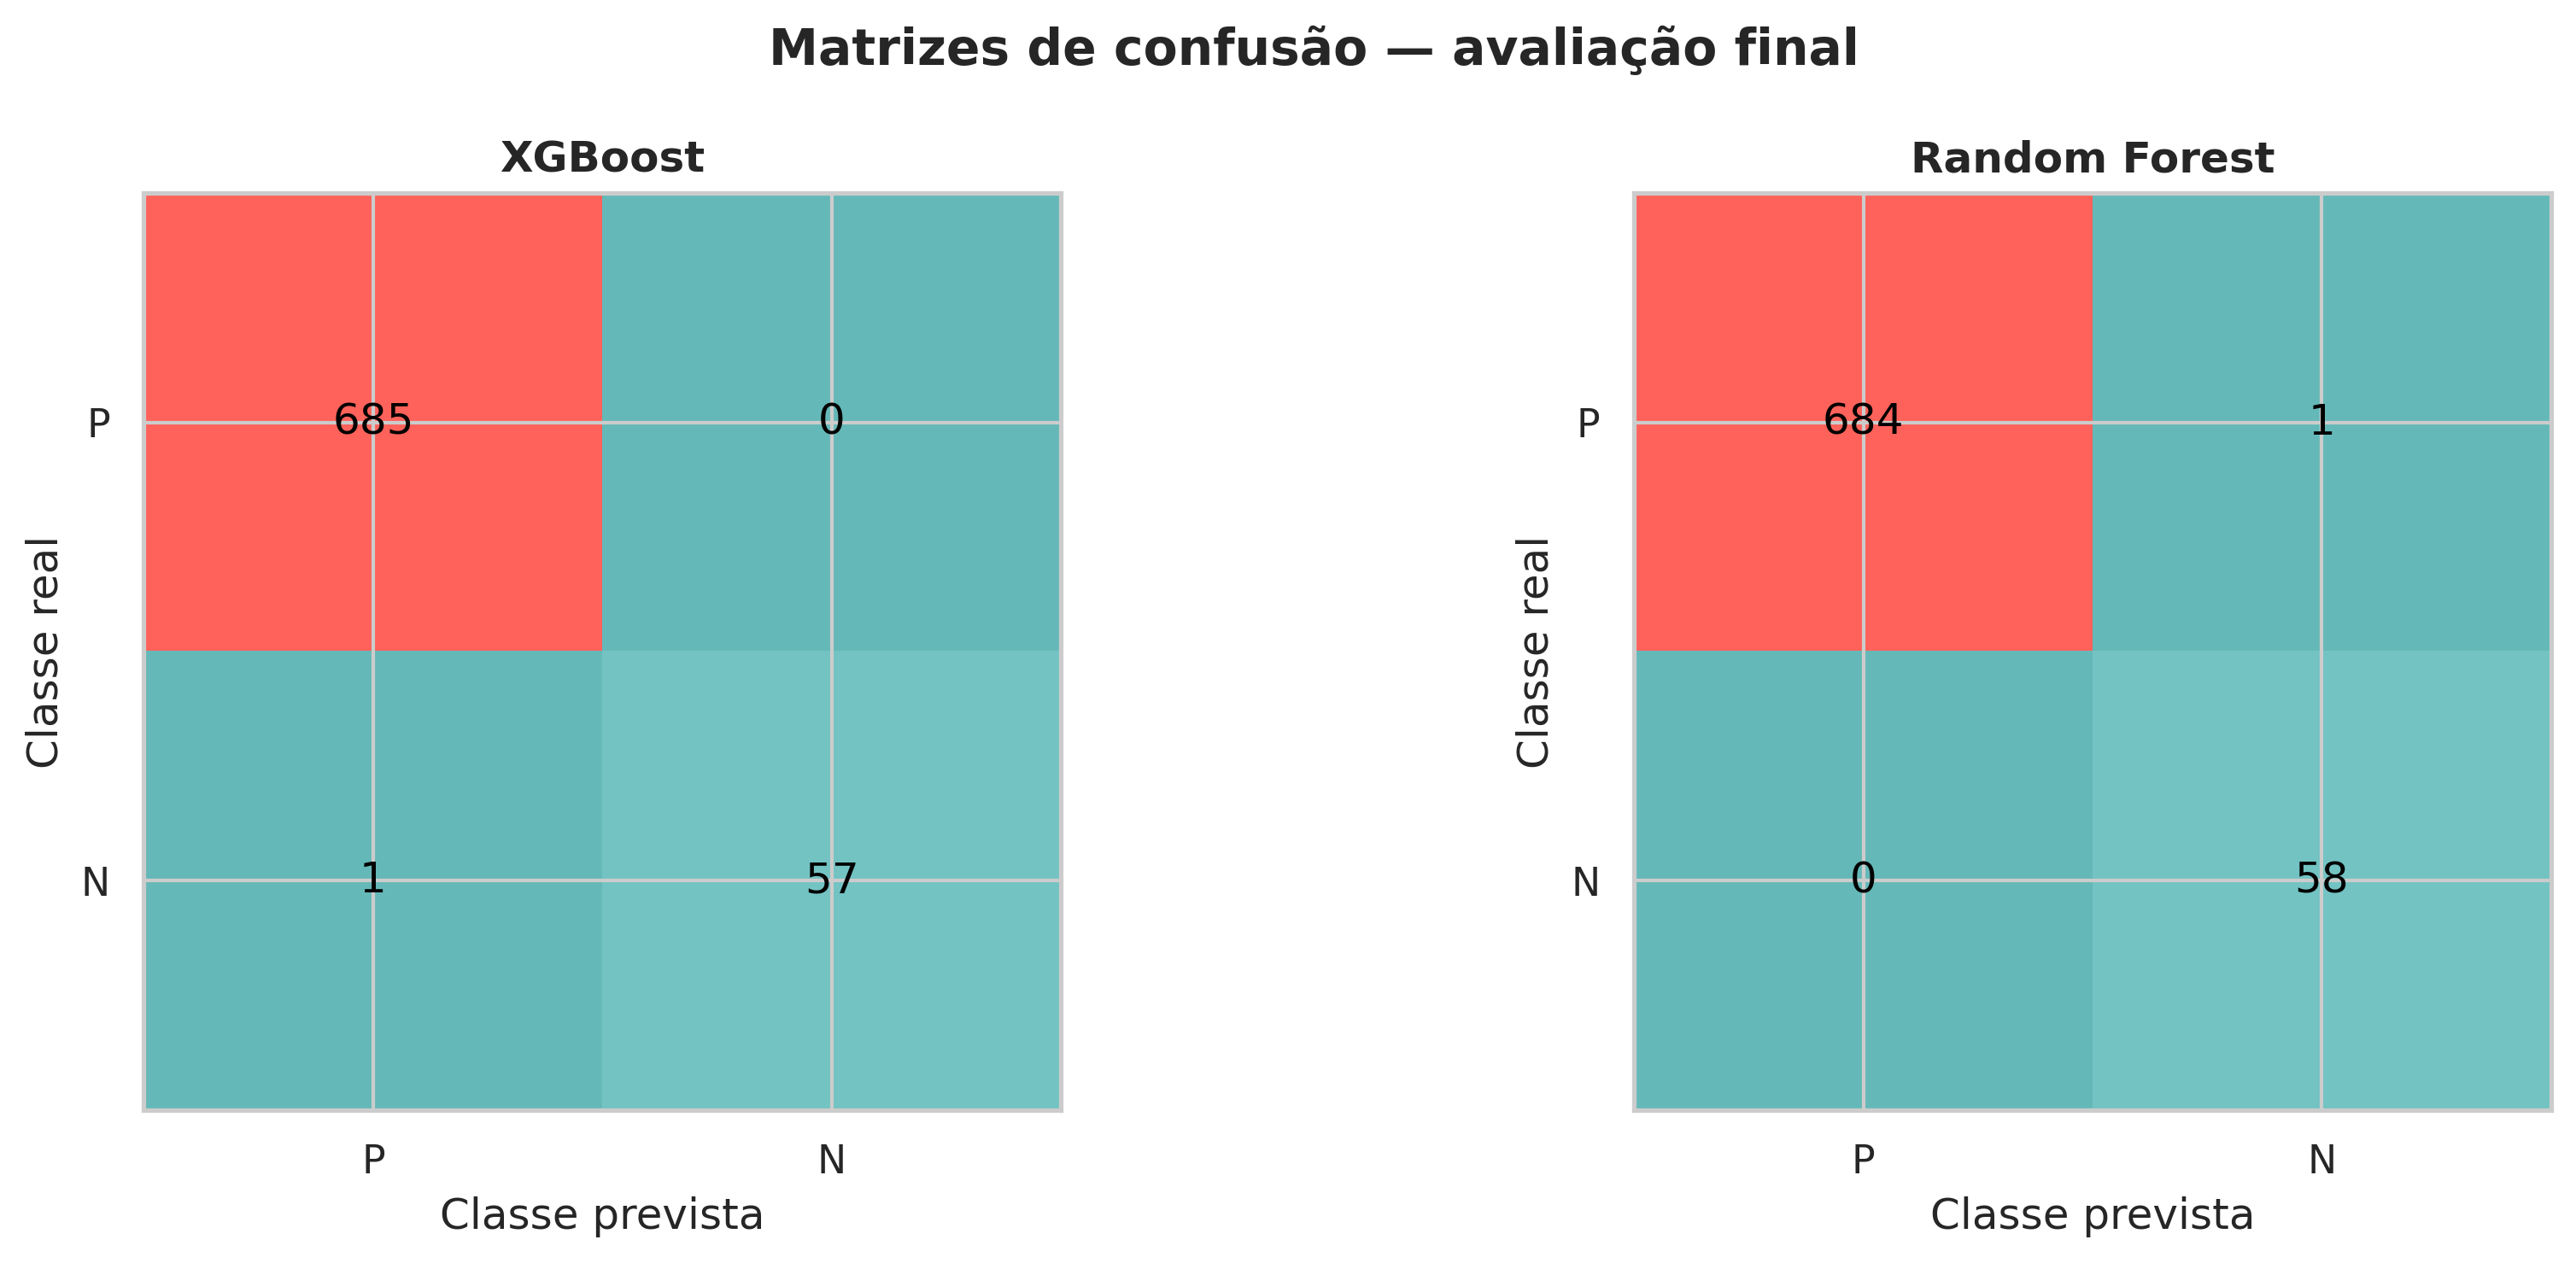
\includegraphics{figuras/ml_07.png}
\caption{Matrizes de confusão}
\end{figure}

Cada modelo apresentou apenas um erro de classificação. O XGBoost
registrou um falso negativo e nenhum falso positivo. O Random Forest
registrou um falso positivo e nenhum falso negativo. Portanto, o XGBoost
não classificou incorretamente registros da classe \texttt{P} como
\texttt{N}, enquanto o Random Forest identificou todos os 58 registros
positivos da validação reservada.

A diferença reflete o equilíbrio entre Precision e Recall observado nos
modelos. Com base nessa avaliação, não há evidência suficiente para
declarar superioridade absoluta de um dos finalistas.

\hypertarget{discussuxe3o}{%
\subsection{11. Discussão}\label{discussuxe3o}}

Os resultados da EDA e da modelagem apontam para a importância dos
indicadores laboratoriais na reprodução da variável-alvo. A diferença
entre as medianas de TSH nas classes e a predominância dessa variável na
importância por permutação são coerentes entre as etapas exploratória e
preditiva.

A análise de sensibilidade reforça essa interpretação: a retirada de TSH
provocou queda expressiva no desempenho de todos os modelos. TT4, FTI e
T3 preservaram informação discriminativa, mas não foram suficientes para
manter os resultados do cenário original.

As variáveis categóricas também apresentaram algumas associações com a
classe, mas com baixa intensidade segundo o V de Cramer. Assim, os
resultados não sustentam a interpretação de que uma única variável
categórica explique a classificação.

Na validação reservada, XGBoost e Random Forest alcançaram métricas
muito elevadas e cometeram apenas um erro cada. Contudo, o desempenho
excepcional deve ser interpretado à luz da origem dos dados e da
definição do alvo. A avaliação demonstra capacidade de reproduzir os
rótulos do conjunto avaliado, mas não estabelece validade clínica ou
generalização para outras populações.

\hypertarget{limitauxe7uxf5es-e-cuidados-de-interpretauxe7uxe3o}{%
\subsection{12. Limitações e cuidados de
interpretação}\label{limitauxe7uxf5es-e-cuidados-de-interpretauxe7uxe3o}}

\begin{enumerate}
\def\labelenumi{\arabic{enumi}.}
\tightlist
\item
  \textbf{Definição da variável-alvo:} a origem e o procedimento de
  construção de \texttt{binaryClass} não foram estabelecidos de forma
  independente. A predominância do TSH entre os preditores e a queda de
  desempenho sem essa variável justificam cautela. Caso o TSH tenha
  participado da definição dos rótulos, pode haver circularidade ou
  vazamento de informação. Os resultados disponíveis não permitem
  confirmar essa hipótese.
\item
  \textbf{Validação interna:} os 743 registros reservados pertencem à
  mesma base de origem dos dados de treinamento. Portanto, a avaliação é
  um holdout interno, não uma validação externa em outra população,
  instituição ou período.
\item
  \textbf{Tamanho da classe positiva:} a classe \texttt{N} possui 233
  registros no treinamento e 58 na validação reservada. O número
  reduzido de positivos limita a precisão das estimativas e exige
  cautela na interpretação das métricas.
\item
  \textbf{Desbalanceamento:} a classe positiva é minoritária. Por isso,
  as métricas devem ser interpretadas em conjunto, sem utilizar acurácia
  isoladamente como critério de qualidade.
\item
  \textbf{Interpretação clínica:} os modelos foram avaliados quanto à
  reprodução dos rótulos presentes na base \texttt{Hypothyroid}. O
  desempenho obtido não comprova capacidade de diagnóstico clínico, não
  substitui avaliação profissional e não demonstra validade em contextos
  reais de atendimento.
\item
  \textbf{Importância dos atributos:} a importância por permutação
  descreve contribuição preditiva no contexto dos modelos ajustados. Não
  representa causalidade ou efeito clínico.
\item
  \textbf{Divisão dos dados:} os resultados finais correspondem a uma
  única divisão estratificada entre treinamento e validação. A
  generalização para outros contextos exigiria avaliação em dados
  independentes.
\end{enumerate}

\hypertarget{conclusuxe3o}{%
\subsection{13. Conclusão}\label{conclusuxe3o}}

A análise exploratória identificou desbalanceamento da variável-alvo,
valores ausentes, duplicatas exatas, uma idade inválida e variáveis sem
informação útil para a modelagem. Também mostrou diferenças entre as
classes nos indicadores laboratoriais, especialmente em TSH, e
correlação positiva entre TT4 e FTI.

Na modelagem, XGBoost e Random Forest apresentaram os melhores
resultados na validação cruzada e foram selecionados para a avaliação
final. O XGBoost obteve F1 médio de 0,966, enquanto o Random Forest
alcançou Recall de 0,991 e PR-AUC de 0,990. Na validação reservada, os
dois modelos apresentaram F1 próximo de 0,99 e apenas um erro de
classificação cada.

A análise de importância por permutação identificou TSH como o principal
preditor nos modelos avaliados. A retirada dessa variável provocou
redução expressiva do desempenho, enquanto TT4, FTI e T3 passaram a
concentrar maior importância relativa no cenário alternativo. As
análises de associação categórica identificaram relações estatísticas de
baixa intensidade para \texttt{on\ thyroxine} e
\texttt{query\ hypothyroid}.

Conclui-se que os modelos apresentam elevada capacidade de reproduzir a
classificação disponível na base analisada. Entretanto, a dependência de
TSH, a necessidade de esclarecer a origem da variável-alvo, o
desbalanceamento e a ausência de validação externa limitam o alcance dos
resultados. Assim, o projeto atende ao objetivo de análise exploratória
e comparação de modelos de classificação sobre os dados disponíveis, mas
não permite afirmar que os algoritmos constituam ferramentas
clinicamente validadas para diagnóstico de hipotireoidismo.

\hypertarget{referuxeancias-e-materiais-do-projeto}{%
\subsection{Referências e materiais do
projeto}\label{referuxeancias-e-materiais-do-projeto}}

\begin{itemize}
\tightlist
\item
  EBAC. \textbf{Proposta do projeto --- Diagnóstico de Hipotireoidismo}.
  Documento de planejamento fornecido para o desenvolvimento do
  trabalho.
\item
  \textbf{Notebook 01 --- Análise Exploratória de Dados (EDA)}.
  Preparação, auditoria, análise exploratória e divisão dos conjuntos.
\item
  \textbf{Notebook 02 --- Modelagem preditiva (ML)}. Pré-processamento,
  validação cruzada, interpretação dos modelos e avaliação final.
\item
  Base de dados: \texttt{Hypothyroid.csv}.
\end{itemize}

\begin{center}\rule{0.5\linewidth}{0.5pt}\end{center}

\hypertarget{organizauxe7uxe3o-sugerida-dos-arquivos}{%
\subsection{Organização sugerida dos
arquivos}\label{organizauxe7uxe3o-sugerida-dos-arquivos}}

\begin{verbatim}
Diagnostico_hipotireoidismo/
├── data/
├── notebook/
│   ├── 01_EDA.ipynb
│   └── 02_ML.ipynb
├── src/
└── docs/
    ├── relatorio_geral.md
    └── figuras/
        ├── eda_01.png
        ├── ...
        ├── eda_12.png
        ├── ml_01.png
        ├── ...
        └── ml_08.png
\end{verbatim}

As referências às imagens neste relatório são relativas ao arquivo
\texttt{relatorio\_geral.md}. Por isso, a pasta \texttt{figuras} deve
permanecer no mesmo diretório \texttt{docs}.

\end{document}
